\documentclass[11pt]{amsbook}
%\documentclass[pdflatex]{amsbook}

\usepackage[ngerman]{babel}
\usepackage[T1]{fontenc}

%\usepackage{ucs}
\usepackage[utf8]{inputenc}

\usepackage{a4}
%\usepackage{fullpage} % UM DEN REGENWALD ZU RETTEN...
\usepackage{amsmath}
\usepackage{amsfonts}
\usepackage{amsthm}
\usepackage{amssymb}
\usepackage{times}
\usepackage{color}
\usepackage{graphicx}

\usepackage{ifthen}
\usepackage{ifpdf}

\usepackage{color,soul} % to highlight text with the command \hl{...}
\definecolor{myhighlightcolor}{gray}{0.92}
\sethlcolor{myhighlightcolor}

\usepackage{pgf,tikz}
\usetikzlibrary{arrows, calc}

% Some general settings
\renewcommand{\baselinestretch}{1.3}
\parindent0mm
\parskip1.2ex

\topmargin-2cm
\textheight24cm
\textwidth15.5cm
\oddsidemargin1.0cm

% EINEN INDEX KOENNTE MAN AUCH NOCH EINBAUEN
% dazu werden im Text einfach die entsprechenden Begriffe mit ``\index{BlaBla}'' gesammelt
%\usepackage{showidx}
%\makeindex

\usepackage[pdfauthor={Achill Schuermann},
            pdftitle={Axiomatische Geometrie},
            pdfsubject={Notizen zur gleichnamigen Vorlesung an der Universitaet Rostock, SS
            2011}]{hyperref}

%\ifpdf
%\pdfinfo{
%   /CreationDate (D:20080506170000)
%}
%\fi

%
% some abbreviations
%

\newcommand{\E}{\mathbb E}
\newcommand{\K}{\mathbb K}
\newcommand{\N}{\mathbb N}
\newcommand{\Z}{\mathbb Z}
\newcommand{\Q}{\mathbb Q}
\newcommand{\R}{\mathbb R}
\newcommand{\C}{\mathbb C}
\renewcommand{\H}{\mathbb H}

\newcommand{\MA}{{\mathcal A}}
\newcommand{\MT}{{\mathcal T}}
\newcommand{\MK}{{\mathcal K}}
\newcommand{\MG}{{\mathcal G}}
\newcommand{\MI}{{\mathcal I}}

%\DeclareMathOperator{\conv}{conv}
%\DeclareMathOperator{\aff}{aff}
%\DeclareMathOperator{\lin}{lin}

%\DeclareMathOperator{\Iso}{Iso}
%\DeclareMathOperator{\Fix}{Fix}
%\DeclareMathOperator{\Id}{Id}

\DeclareMathOperator{\Zw}{Zw}
\DeclareMathOperator{\dist}{dist}
\DeclareMathOperator{\Rang}{Rang}
\DeclareMathOperator{\Rot}{Rot}
\DeclareMathOperator{\Ref}{Ref}

\DeclareMathOperator{\Real}{Re}
\DeclareMathOperator{\Imag}{Im}

%\newcommand{\dr}{\mbox{${\scriptstyle\triangle}$}}
        %Dreieck
%\newcommand{\sdr}{\mbox{${\scriptstyle\triangle}_S$}}
        %sphärisches Dreieck
\newcommand{\wi}{\mbox{$\measuredangle$}}
        %Winkel
%\newcommand{\swi}{\mbox{${\scriptstyle\angle}_S$}}
        %sphärischer Winkel
%\newcommand{\olS}[1]{\mbox{${\overline{#1}\,^S}$}}
        %sphärische Strecke
\newcommand{\pf}[1]{\mbox{${\overrightarrow{#1}}$}}
        %Strahl
\newcommand{\str}[1]{{#1}}
        %Strecke
%\newcommand{\strm}[1]{{#1}}
%       %Strecke (math. Modus)

\newcommand{\ve}[2]{\begin{pmatrix}{#1}\\{#2}\end{pmatrix}}
        %zweizeiliger Spaltenvektor
\newcommand{\ved}[3]{\begin{pmatrix}{#1}\\{#2}\\{#3}\end{pmatrix}}


%% EIN EIGENER theoremstyle (instead of the nonboldface ones of amsbook)
\newtheoremstyle{mythmstyle}% name
    {8pt}       % Space above
    {8pt}       % Space below
    {\itshape}  % Body font
    {\parindent}% Indent amount (empty = no indent, \parindent = para indent)
    {\bfseries} % Thm head font  (+ \scshape ??)
    {.}         % Punctuation after thm head
    {.5em}      % Space after thm head: " " = normal interword space;
                % \newline = linebreak
    {}          % Thm head spec (can be left empty, meaning `normal')

\theoremstyle{mythmstyle}
\newtheorem{defi}{DEF}[section]
%\newtheorem{proposition}[defi]{PROP}
%\newtheorem{lemma}[defi]{Lemma}
\newtheorem{thm}[defi]{THM}
%\newtheorem{korollar}[def]{Korollar}
\newtheorem{bem}[defi]{BEM}

\newtheorem{konst}[defi]{KONSTRUKTION}

%% Ohne Nummerierung
\theoremstyle{definition}
\newtheorem*{bsp}{BSP}

% Ein paar Parameter um mit der Nummerierung und dem Inhaltsverzeichnis zu spielen:
\setcounter{tocdepth}{1}
%\renewcommand{\thesection}{\arabic{chapter}.\arabic{section}}
\renewcommand{\thesection}{\arabic{chapter}}

% ==========================
% = Authors / Affiliations =
% ==========================

\author{Prof. Dr. Achill Schürmann}
%\address{Achill Sch\"urmann, Institute for Mathematics, University of Rostock, 18051 Rostock, Germany}
%\email{Achill.Schuermann@uni-rostock.de}

\title[Axiomatische Geometrie]{Axiomatische Geometrie}

\begin{document}

% vim:tw=100:ts=4:sw=4:sts=4:et:
\thispagestyle{empty}
\vspace*{3cm}

\begin{center}
	{\Large Notizen zur Vorlesung\\}
	\vspace{1cm}
	{\LARGE{\bf Axiomatische Geometrie}\\}
	\vspace{1.5cm}

{\Large
   gehalten im SS 2011 an der \\[1cm]
     U n i v e r s i t ä t  \quad  R o s t o c k\\[1cm]
   von \\[1cm]
    \href{http://www.geometrie.uni-rostock.de/}{Prof. Dr. Achill Schürmann}\\[1cm]
}
\end{center}

\vspace{4cm}

\noindent
{\bf Warnung:} Dieser Text befindet sich in laufender Überarbeitung.
%Auf den \href{https://studip.uni-rostock.de/}{Stud.IP-Seiten} zur Vorlesung
%finden Sie die jeweils aktuelle Version. 
Über Hinweise auf Fehler, oder allgemein zur Verbesserung der Materialien, freue ich mich sehr!

\vspace{2cm} 

\noindent

(Fassung vom \today)

%% Inhaltsverzeichnis fuer die Gesamtversion

%\newpage

%\vspace*{1cm}
%\noindent

%{\large\tableofcontents}


%%% Local Variables: 
%%% mode: latex
%%% TeX-master: "AxiomatischeGeometrie.tex"
%%% End: 


%\maketitle

%\tableofcontents

%\chapter*{Was soll das alles?}
%\input{WasSollDasAlles.tex}

\chapter{Euklid}
\section*{Vorlesung am 05.04.2011}

\subsection*{Euklid von Alexandria}

\begin{itemize}
\item Ursprünge der Geometrie; Landvermessung, Architektur in frühen Hochkulturen
\item \href{http://www.opera-platonis.de/euklid/}{Euklids Elemente} (ca. 300 vor Christus); über mit
    Zirkel und Lineal ausführbare Konstruktionen; fasst das Wissen seiner Zeit zusammen. Das Werk
    ist geprägt von griechischer Naturphilosophie (Platon's Ideenlehre).
\item Euklids Werk ist und wegweisend für das moderne wissenschaftliche Denken, insbesondere für den
    Aufbau der modernen, abstrakten Mathematik. Er begründet die "`Axiomatische Methode"': Ausgehend
    von einer kleinen Anzahl von Definitionen und Annahmen (Axiomen / Postulaten) werden logische
    Schlußfolgerungen gezogen. Dies setzt natürlich eine (implizite) Einigung auf die verwendeten
    Prinzipien der Logik voraus!
\item Buch I der Elemente beginnt mit einigen "`Erklärungen"'\ (Definitionen). Es werden
    insbesondere die Begriffe {\em Punkt}, {\em Strecke}, {\em Gerade}, {\em Fläche}, {\em (rechter)
    Winkel}, {\em Dreieck}, {\em Quadrat}, {\em Senkrechte} und {\em Parallele} "`erklärt"'.  Diese
    Erklärungen sind (von einem modernen Standpunkt aus) wenig erhellend.
\end{itemize}

\subsection*{Konstruktionen mit Zirkel und Lineal}

In Buch I, folgen auf die Erklärungen "`Erste Folgerungen"' (Konstruktions-Axiome).

\renewcommand{\labelenumi}{\arabic{enumi}.} % ändert die Nummerierung von (1) auf 1.
\begin{enumerate}
    \item Von einem beliebigen Punkt zu einem anderen kann eine gerade Strecke gezogen werden,
    \item und eine gerade Strecke ist beliebig verlängerbar,
    \item und um einen beliebigen Punkt ist mit beliebigem Radius ein Kreis beschreibbar,
    \item \dots
\end{enumerate}

In modernen Texten werden 1. und 2. oft zusammengefasst: Durch je zwei verschiedene Punkte lässt
sich eine Gerade legen.
% Durch "beliebig verlängerbar" vermeidet Euklid das "Unendliche"!
Sie ermöglichen die Konstruktion von Strecken und Geraden mit einem {\em Lineal}.

Die Möglichkeit zur Konstruktion eines Kreises wird durch 3. gegeben. Ein "`beliebiger Radius"' kann
dabei nicht als eine reelle Zahl (im modernen Sinne) interpretiert werden, sondern immer nur als
Radius (Länge) $|AB|$ zwischen zwei gegebenen Punkten $A$ und $B$. Euklid geht von einem
"`vergesslichen Zirkel"' aus, d.h. einem Zirkel der die Länge $|AB|$ nicht "`speichern"' kann, wenn
er nicht an einem der beiden Punkte $A$ oder $B$ anliegt. In Abschnitt (Konstruktion) I.2 zeigt er
allerdings, dass dies keine Einschränkung gegenüber einem Zirkel ist, der Radien übertragen kann.

{\em Kritik:} Auch wenn es nicht explizit erwähnt wird, werden zusätzliche
Konstruktionsmöglichkeiten angenommen. Zum Beispiel lassen sich neue Punkte "`zufällig"' erzeugen
oder mit bestimmten Eigenschaften, etwa dass sie "`auf einer Geraden"' oder "`auf einem Kreis"'
liegen, oder auch "`auf der anderen Seite einer Geraden"' (bezogen auf einen bereits existierenden
Punkt), etc \dots.

\subsection*{Konstruktion des gleichseitigen Dreiecks}

Der erste Abschnitt I.1 in Euklids Elementen beginnt mit der Konstruktion eines gleichseitigen
Dreiecks. Ein gleichseitiges Dreieck ist nach Euklid ein Dreieck in dem alle Strecken "`gleich
sind"'. Mit Gleichheit von Strecken ist dabei Gleichheit ihrer Längen gemeint (Kongruenz).

\begin{konst}[Gleichseitiges Dreieck, I.1]\ \\
    Gegeben: Strecke $AB$\\
    Resultat: gleichseitiges Dreieck $ABC$

    \renewcommand{\labelenumi}{\arabic{enumi}.} % ändert die Nummerierung von (1) auf 1.
    \begin{enumerate}
        \item Konstruiere den Kreis $\MK(A,|AB|)$
        \item Konstruiere den Kreis $\MK(B,|BA|)$
        \item $C$ sei einer der beiden Schnittpunkt von $\MK(A,|AB|)$ und $\MK(B,|BA|)$
        \item Konstruiere die Strecke $AC$
        \item Konstruiere die Strecke $BC$
        %\item[6.] Konstruiere das Dreieck $ABC$
    \end{enumerate}
\end{konst}

\begin{figure}[h]
    % Konstruktion gleichseitiges Dreieck
% (genau diese Konstruktion wird im PGF/TikZ Manual beschrieben - warum nicht die eingebauten
% Features nutzen?)
% Änderungen sind eigentlich nur an den Koordinaten der Punkte oder am 'scale'-Faktor nötig. Den
% Rest erledigt TikZ selbst.
\begin{tikzpicture}[line cap=round,line join=round,x=1.0cm,y=1.0cm,scale=1.0]
    % Punkt A mit Beschriftung
    \coordinate (A) at (0,0);
    \fill [color=colPkt] (A) circle (1.5pt);
    \draw [color=colPkt, anchor=north east] (A) node {$A$};
    % Punkt B mit Beschriftung
    \coordinate (B) at (2,0);
    \fill [color=colPkt] (B) circle (1.5pt);
    \draw [color=colPkt, anchor=north west] (B) node {$B$};
    % Kreise "um A durch B" und "um B durch A"
    \node (KA) [draw, circle through=(B)] at (A) {};
    \node (KB) [draw, circle through=(A)] at (B) {};
    % Schnittpunkt der Kreise
    \coordinate (C) at (intersection 2 of KA and KB);
    \fill [color=colPktKon] (C) circle (1.5pt);
    \draw [color=colPktKon, anchor=south] (C) node {$C$};
    % das gleichseitige Dreieck
    \draw (A)--(B)--(C)--(A);
\end{tikzpicture}

    \caption{Konstruktion eines gleichseitigen Dreiecks}
\end{figure}

{\em Kritik:} Ein häufig angeführter Kritikpunkt an Euklids Werk betrifft die implizit angenommene
Existenz eines Schnittpunkts $C$.

%Solche implizit gemachten Annahmen, die anschaulich klar scheinen
%verwässern (von einem modernen Standpunkt) den axiomatischen Ansatz Euklids

Euklid trennt hier und in den folgenden Abschnitten zwischen der Konstruktion und dem Beweis.

\begin{proof}
    Nach Konstruktion gilt $|AB|=|AC|$ und $|BC|=|BA|$.
    Da $|AB|=|BA|$ folgt auch (wegen der Transitivität von "`$=$"' ) $|BC|=|AC|$.
\end{proof}

Die Konstruktion des gleichseitigen (regelmäßigen) Dreiecks wirft die Frage auf, ob sich auch andere
regelmäßige Polygone mit Zirkel und Lineal konstruieren lassen. Die Antwort hierauf ist überraschend
kompliziert und wurde von Gauß (im Alter von 26)
% bereits als 19jähriger den Primzahlfall gelöst!
abschließend geklärt.
% MEHR INFO...

\begin{thm}[Gauß, 1801]  % Satz von Gauß-Wantzel!!?!?!!
    Das regelmäßige $n$-Eck lässt sich mit Zirkel und Lineal genau dann konstruieren, wenn
    $$
        n = 2^k \cdot \mbox{"`Produkt verschiedener Fermat-Zahlen"'}.
    $$
    Dabei ist eine Fermat-Zahl eine Primzahl der Form $2^{2^m}+1$.
\end{thm}

Bis heute sind nur die fünf Fermat-Zahlen $3$,$5$, $17$, $257$ und $65537$ ($m=0,\ldots,4$) bekannt!

\subsection*{Radien übertragen}

In Euklids zweitem Abschnitt I.2 wird eine Konstruktion angegeben, die zeigt, dass ein
"`vergesslicher Zirkel"' die gleichen Fähigkeiten hat wie ein Zirkel, der Radien (Längen) zwischen
zwei Punkten $B$ und $C$ speichern und an einem gegebenen Punkt $A$ abtragen kann.

\begin{konst}[Strecke mit bekanntem Radius, I.2]\ \\
    Gegeben: Punkt $A$, Strecke $BC$ \\
    Resultat: Strecke $AF$ mit $|AF|=|BC|$
    \renewcommand{\labelenumi}{\arabic{enumi}.} % ändert die Nummerierung von (1) auf 1.
    \begin{enumerate}
        \item Konstruiere Strecke $AB$
        \item Konstruiere gleichseitiges Dreieck $ABD$ (Euklids I.1, s.o.)
        \item Konstruiere Gerade $g$ durch $B$ und $D$
        \item Konstruiere Kreis $\MK(B,|BC|)$
        \item $E$ sei der Schnittpunkt von $g$ und $\MK(B,|BC|)$, mit $B$ {\em zwischen} $E$ und $D$
        \item Konstruiere Gerade $h$ durch $A$ und $D$
        \item Konstruiere Kreis $\MK(D,|DE|)$
        \item $F$ sei der Schnittpunkt von $h$ und $\MK(D,|DE|)$
    \end{enumerate}
\end{konst}

{\em Kritik:} Man beachte, das die Existenz eines Schnittpunktes von Gerade und Kreis angenommen
wird. Außerdem wird angenommen, dass dieser "`zwischen"' zwei anderen Punkten liegt.

\begin{proof}
    Nach Konstruktion gilt $|BC|=|BE|$, $|DE|=|DF|$ und $|DB|=|DA|$.
    Es folgt (nach Euklids "`Grundsätzen"')
    $$
        |AF|=|DF|-|DA|= |DE|-|DB| = |BE| = |BC|.
    $$
\end{proof}

%\subsection*{Addition und Subtraktion von Längen}

In Euklids Abschnitt I.3 wird die Subtraktion von Strecken (für uns Längen) erklärt.

\begin{konst}[Subtraktion von Längen, I.3]\ \\
    Gegeben: Strecken $AB$ und $CD$ mit  $|AB| > |CD|$ \\
    Resultat: Strecke $AE$ mit $|AE|=|AB|-|CD|$
    \renewcommand{\labelenumi}{\arabic{enumi}.} % ändert die Nummerierung von (1) auf 1.
    \begin{enumerate}
        \item Konstruiere Kreis $\MK(A,|CD|)$ (Euklid I.2, s.o.)
        \item Konstruiere Gerade $g$ durch $A$ und $B$
        \item $E$ sei der Schnittpunkt von $g$ und $\MK(A,|CD|)$ {\em zwischen} $A$ und $B$
    \end{enumerate}
\end{konst}

Addition von Längen erhält man durch den anderen Schnittpunkt der Geraden und des Kreises in der
obigen Konstruktion. Das ermöglicht die Skalierung einer Geraden.
% durch wiederholte Addition.
% Man beachte, dass Längen immer nur im Verhältnis zu Punkten gegeben sind (Propotionslehre bla bla)

\subsection*{Kongruenzaxiome}

Was bei Euklid in Abschnitt I.4 behandelt wird, ist heute auch als {\em SWS-Kriterium} bekannt.

{\em Kritik:} Für den Beweis setzt Euklid implizit ein Konzept der Bewegung (Superposition) voraus,
das axiomatisch schwierig zu fassen ist. Heute wird das SWS-Kriterium deshalb häufig als Axiom
formuliert.

% TODO: Kritik an Superposition besser untermauern... (siehe Hartshorne)

\begin{description}
    \item[SWS-Axiom] Wenn für zwei Dreiecke $ABC$ und $A'B'C'$ gilt $|AB|=|A'B'|$, $\angle ABC =
        \angle A'B'C'$ und $|BC|=|B'C'|$, so gilt auch $|AC|=|A'C'|$ und $\angle ABC = \angle
        A'B'C'$
\end{description}

Das entsprechende {\bf WSW-Kriterium} und das {\bf SSS-Kriterium} können aus dem {\bf
SWS-Kriterium} hergeleitet werden. Man beachte, dass es kein allgemeines SSW-Kriterium gibt. Mit
der zusätzlichen Einschränkung, dass die längste Seite und der gegenüberliegende Winkel bekannt
sind, kann man allerdings ein Kriterium angeben (das in der Schule manchmal auch als SsW-Kriterium
bezeichnet wird).

\section*{Vorlesung am 07.04.2011}

Der folgende Satz ist eine einfache Folgerung aus dem SWS-Kriterium (Euklid, I.5):

\begin{thm}[über das gleichseitige Dreieck]
    Wenn ein Dreieck zwei gleiche (kongruente) Seiten hat, dann sind die gegenüberliegenden Winkel
    auch gleich (kongruent).
\end{thm}

% Beweis von Pappus: (Schreckliche Formulierung / muss überarbeitet werden)
%\begin{proof}
%Angenommen in einem Dreieck ABC gilt $|AB|=|AC|$. Dann sind in den
%Dreiecken BAC und CAB (die beide mit ABC identisch sind) nicht nur zwei Seiten, sondern auch der
%eingeschlossene Winkel $\angle BAC = \angle CAB$ identisch. Nach dem SWS-Kriterium sind dann auch
%die anderen Winkel identisch. Da wir diese in unterschiedlicher
%Reihenfolge durchlaufen, sind sie also beide (alle vier) gleich.
%\end{proof}

\subsection*{Konstruktion von Lot und Parallele}

Aufbauend auf der Konstruktion des gleichseitigen Dreiecks lässt sich auch leicht ein Lot zu einer
Geraden konstruieren.
%durch zwei Punkte $A$ und $B$

\begin{konst}[Lot einer Geraden]\ \\
    Gegeben: Gerade $g$ und ein Punkt $E$ auf $g$\\
    Resultat: Gerade $h$ durch $E$, die senkrecht zu $g$ ist
    \renewcommand{\labelenumi}{\arabic{enumi}.} % ändert die Nummerierung von (1) auf 1.
    \begin{enumerate}
        \item Wähle einen Punkt $A \neq E$ auf $g$
        \item Konstruiere Kreis $\MK(E,|AE|)$
        \item $B \neq A$ sei der andere Schnittpunkt der Geraden $g$ und $\MK(E,|AE|)$
        \item Konstruiere Kreis $\MK(A,|AB|)$
        \item Konstruiere Kreis $\MK(B,|BA|)$
        \item $C$ und $D$ seien die beiden Schnittpunkte von $\MK(A,|AB|)$ und $\MK(B,|BA|)$
        \item Konstruiere Gerade $h$ durch $C$ und $D$
    \end{enumerate}
\end{konst}

% \begin{konst}[Zweiteilung einer Strecke]
% % Euklid I.10
% %BEMERKUNG: Bei Euklid wird die Zweiteilung der Strecke erst nach der
% %Zweiteilung des Winkels behandelt...
% \phantom{Pups}\hspace*{1cm}\phantom{Pups}\\
% \underline{Gegeben:} Strecke $AB$\\
% \underline{Resultat:} Punkt $E$ auf $AB$ mit $|AE|=|EB|$
% \begin{enumerate}
% \item[1.] Konstruiere Kreis $\MK(A,|AB|)$
% \item[2.] Konstruiere Kreis $\MK(B,|BA|)$
% \item[3.] $C$ und $D$ seien die beiden Schnittpunkte von $\MK(A,|AB|)$
%   und $\MK(B,|BA|)$
% \item[4.] Konstruiere Gerade $g$ durch $A$ und $B$
% \item[5.] Konstruiere Gerade $h$ durch $C$ und $D$
% \item[6.] $E$ sei der Schnittpunkt der Geraden $g$ und $h$
% \end{enumerate}
% \end{konst}

%% BEWEIS???

\begin{figure}[h]
    \begin{tikzpicture}[line cap=round,line join=round,x=1.0cm,y=1.0cm,scale=0.5]
    \clip(-4,-3) rectangle (5,6);
    \draw [color=colPktKon] (-0.44,0.29) coordinate (A) node[anchor = north east] {$A$};
    \draw [color=colPktKon] (1.48,-0.10) coordinate (B) node[anchor = north west] {$B$};
    \draw [color=colPktKon] (0.85,1.75) coordinate (C) node[anchor = north west] {$C$};
    \draw [color=colPktKon] (0.19,-1.56) coordinate (D) node[anchor = east] {$D$};
    \draw [color=colPkt] (1,2.5) coordinate (E) node[anchor = south west] {$E$};
    \draw [dash pattern=on 2pt off 2pt](E) circle (2.64cm);
    \draw [dash pattern=on 1pt off 1pt] (A) circle (1.95cm);
    \draw [dash pattern=on 1pt off 1pt] (B) circle (1.95cm);
    \draw [color=colPkt] (4.24,-0.56) node[anchor = south] {$g$};
    \draw (1.64,5.68) node[anchor = west] {$h$};
    \draw [line width = 1pt,domain=-4:6] plot(\x,{(--2-2*\x)/10});
    \draw [line width = 1pt,domain=-4:6] plot(\x,{(-1.66--3.32*\x)/0.66});
    \fill [color=colPkt] (E) circle (1.5pt);
    \fill [color=colPktKon] (A) circle (1.5pt);
    \fill [color=colPktKon] (B) circle (1.5pt);
    \fill [color=colPktKon] (C) circle (1.5pt);
    \fill [color=colPktKon] (D) circle (1.5pt);
\end{tikzpicture}

    \caption{Lot einer Geraden}
\end{figure}

Die letzten vier Schritte der Konstruktion lassen sich auch verwenden um eine gegebene Strecke $AB$
in zwei gleich große Teile zu teilen (Mittelsenkrechte).

% An dieser Stelle lässt sich eine schöne Aufgabe stellen:
% Die Mittelsenkrechten in einem Dreieck schneiden sich alle in einem Punkt.
% (Beweis mittels Kongruenz-Kriterien?!)

\begin{proof}
    Nach Konstruktion haben die Dreiecke $AEC$ und $BEC$ drei gleich lange Seiten. Nach dem
    SSS-Kriterium sind sie deshalb kongruent. Ihre Winkel bei $E$ (die Schnittwinkel von $g$ und
    $h$) sind daher gleich (kongruent). Dies definiert nach Euklid eine Senkrechte (und rechte
    Winkel).
    % Referenz / Hinweis auf Euklid's Definition?
\end{proof}

Für einen Punkt $E$ außerhalb einer Geraden $g$ lässt sich in ähnlicher Weise eine Senkrechte $h$
auf $g$ durch $E$ konstruieren. Dabei ist nur zu beachten, dass der Kreis um $E$ groß genug ist, um
zwei verschiedene Schnittpunkte $A$ und $B$ mit der Geraden $g$ zu haben.

Die Konstruktion einer {\em Senkrechten} ({\em Lot}) $h$ zur Geraden $g$ lässt sich auch verwenden,
um in zwei Schritten eine {\em Parallele} zu $g$ zu konstruieren (d.h., eine von $g$ verschiedene
Gerade, die keinen Schnittpunkt mit $g$ besitzt).

\begin{konst}[Parallele einer Geraden]\ \\
    Gegeben: Gerade $g$ und ein Punkt $E$ außerhalb von $g$\\
    Resultat: Gerade $g'$ durch $E$, die parallel zu $g$ liegt
    \renewcommand{\labelenumi}{\arabic{enumi}.} % ändert die Nummerierung von (1) auf 1.
    \begin{enumerate}
        \item Konstruiere Senkrechte $h$ auf $g$ durch $E$
        \item Konstruiere Senkrechte $g'$ auf $h$ durch $E$
    \end{enumerate}
\end{konst}

Ein Beweis der Parallelität aus den bisher behandelten Konstruktions-Axiomen ist nicht möglich!
% Referenzen??
%% Wurde über Jahrhunderte versucht zu beweisen aus anderen Axiomen...
Dafür ist Euklids {\bf Parallelenaxiom} notwendig (Buch I, Erste Folgerungen, 5.).
\begin{quote}
Wenn eine Gerade %$h$
zwei Geraden %$g$ und $g'$
schneidet und auf einer Seite die Winkel
%$\alpha$ und $\beta$
zusammen weniger als zwei Rechte ($<\pi$) sind, dann scheiden sich die beiden Geraden auf der Seite.
\end{quote}

\begin{figure}[h]
    \begin{tikzpicture}[line cap=round,line join=round,>=triangle 45,x=1.0cm,y=1.0cm]
    \clip(-2,-1) rectangle (6,4);
    \draw [shift={(0.2,0)},color=colWin,fill=colWin,fill opacity=0.1] (0,0) -- (0:0.6)
        arc (0:78.69:0.6) -- cycle;
    \draw [shift={(0.69,2.47)},color=colWin,fill=colWin,fill opacity=0.1] (0,0) -- (-101.31:0.6)
        arc (-101.31:-8.13:0.6) -- cycle;
    \draw [domain=-2:6] plot(\x,{(-0-0*\x)/7});
    \draw [domain=-2:6] plot(\x,{(--18-1*\x)/7});
    \draw [domain=-2:6] plot(\x,{(-1--5*\x)/1});
    \draw[color=colWin] (0.45,0.2) node {$\alpha$};
    \draw[color=colWin] (0.85,2.2) node {$\beta$};
    \draw[color=black] (3.78,0) node[anchor = north] {$g$};
    \draw[color=black] (3.78,2) node[anchor = north] {$g'$};
    \draw[color=black] (0.09,-0.53) node[anchor = west] {$h$};
\end{tikzpicture}

    \caption{Parallelenaxiom}
\end{figure}

Aus dem Parallelenaxiom lassen sich einige vertraute Aussagen herleiten:

\begin{thm}
    Wenn eine Gerade $h$ zwei parallele Geraden %$g$ und $g'$
    schneidet, dann gilt
    \begin{enumerate}
        \item $\alpha + \beta = \pi$ für zwei benachbarte Winkel $\alpha$ und $\beta$  auf einer
        Seite von $h$.
        % irgendeiner der Geraden
        \item Die inneren Wechselwinkel an $h$ sind gleich (kongruent).
        \item {\em Innenwinkelsatz}: Die Summe der Innenwinkel in einem Dreieck ist $\pi$.
        % (2Rechte).
    \end{enumerate}
\end{thm}

\begin{figure}[h]
    \begin{tabular}{cc}
        \begin{tikzpicture}[line cap=round,line join=round,x=1.0cm,y=1.0cm]
    \clip (-2,-1) rectangle (5,3);
    \draw [shift={(0.86,0)},color=colWin,fill=colWin,fill opacity=0.1] (0,0) -- (0:0.6)
        arc (0:74.05:0.6) -- cycle;
    \draw [shift={(0.86,0)},color=colWin,fill=colWin,fill opacity=0.1] (0,0) -- (180:0.6)
        arc (180:74.05:0.6) -- cycle;
    \draw [shift={(1.43,2)},color=colWin,fill=colWin,fill opacity=0.1] (0,0) -- (-105.95:0.6)
        arc (-105.95:0:0.6) -- cycle;
    \draw [shift={(1.43,2)},color=colWin,fill=colWin,fill opacity=0.1] (0,0) -- (-180:0.6)
        arc (-180:-105.95:0.6) -- cycle;
    \draw [domain=-2:5] plot(\x,{(-0-0*\x)/7});
    \draw [domain=-2:5] plot(\x,{(--14-0*\x)/7});
    \draw [domain=-2:5] plot(\x,{(-6--7*\x)/2});
    \draw [color=colWin] (1.15,0.15) node {\footnotesize $\alpha$};
    \draw [color=colWin] (0.6,0.15) node {\footnotesize $\pi$-$\alpha$};
    \draw [color=colWin] (1.08,1.8) node {\footnotesize $\alpha$};
    \draw [color=colWin] (1.7,1.8) node {\footnotesize $\pi$-$\alpha$};
    \draw [color=black] (3.6,0) node[anchor = north] {$g$};
    \draw [color=black] (4.2,2) node[anchor = north] {$g'$};
    \draw [color=black] (0.65,-.72) node[anchor = west] {$h$};
\end{tikzpicture}

        &
        \begin{tikzpicture}[line cap=round,line join=round,>=triangle 45,x=1.0cm,y=1.0cm]
    \clip (0,0.5) rectangle (7,4.5);
    \draw [shift={(1,1)},color=colWin,fill=colWin,fill opacity=0.1] (0,0) -- (0:0.6)
        arc (0:42.27:0.6) -- cycle;
    \draw [shift={(6,1)},color=colWin,fill=colWin,fill opacity=0.1] (0,0) -- (119.54:0.6)
        arc (119.54:180:0.6) -- cycle;
    \draw [shift={(4.3,4)},color=colWin,fill=colWin,fill opacity=0.1] (0,0) -- (-137.73:0.6)
        arc (-137.73:-60.46:0.6) -- cycle;
    \draw [shift={(4.3,4)},color=colWin,fill=colWin,fill opacity=0.1] (0,0) -- (-180.00:0.6)
        arc (-180.0:-137.73:0.6) -- cycle;
    \draw [shift={(4.3,4)},color=colWin,fill=colWin,fill opacity=0.1] (0,0) -- (-60.46:0.6)
        arc (-60.46:0:0.6) -- cycle;
    \draw (1,1)-- (6,1);
    \draw (6,1)-- (4.3,4);
    \draw (4.3,4)-- (1,1);
    \draw [dash pattern=on 2pt off 2pt,domain=0:7] plot(\x,{(--20-0*\x)/5});
    \draw [color=colWin] (1.4,1.15) node {\footnotesize $\alpha$};
    \draw [color=colWin] (3.87,3.83) node {\footnotesize $\alpha$};
    \draw [color=colWin] (5.67,1.2) node {\footnotesize $\beta$};
    \draw [color=colWin] (4.65,3.75) node {\footnotesize $\beta$};
    \draw [color=colWin] (4.25,3.6) node {\footnotesize $\gamma$};
\end{tikzpicture}

    \end{tabular}
    \caption{Winkel an Parallelen und am Dreieck}
\end{figure}

%\begin{proof}
% Fall 1: Wäre es kleiner, wäre es entweder keine Gerade
% Fall 2: oder die zwei parallelen Geraden würden sich auf der
% entsprechenden Seite schneiden...
% Man beachte, dass bekannt sein muss, dass zwei benachbarte Winkel an einer
% Geraden in der Summe $\pi$ ergeben
%\end{proof}

%% FOLGERUNG:
%Aus dem Satz lässt sich leicht folgern, dass sich die
%Innenwinkel in einem Dreieck zu $\pi$ addieren.
% BILD!! (Stillwell, S. 23)

Eine häufig verwendete, äquivalente Formulierung des Parallelenaxioms\footnote{nach John Playfair,
1795} lässt sich aus dem Parallelenaxioms Euklids herleiten:

\begin{thm}
    Für eine Gerade $g$ und einen Punkt $E$ außerhalb von $g$ gibt es genau eine Gerade durch $E$,
    die $g$ nicht schneidet.
\end{thm}

%% Ist dieses Theorem auch äquivalent zum Parallelenaxiom??
%% Wenn ja, wie sieht der Beweis aus? (Übung??)
%%
%% Man kann auch ".. gibt es höchstens eine Gerade .." als Axiom
%% fordern und dann mit anderen Axiomen die obige Aussage herleiten.
%% Siehe zum Beispiel Nesselmann-Skript, Abschnitt 1.4

\begin{proof}
Sei $h$ eine Gerade durch $E$, die $g$ schneidet. % zum Beispiel das Lot

{\em Eindeutigkeit:} Eine Parallele $g'$ zu $g$ durch $E$ schließt bei $E$ einen festen Winkel ein
(der nur von $g$ und $h$ abhängt). Damit ist die Gerade festgelegt.

{\em Existenz:} Über WSW-Kriterium:

Angenommen es existiert ein Schnittpunkt auf einer Seite von $h$. Die beiden eingeschlossenen
Winkel auf diese Seite von $h$ sind $\alpha$ und $\pi-\alpha$. Dann gibt es nach dem WSW-Kriterium
auch einen Schnittpunkt $D$ auf der anderen Seite von $h$. Das widerspricht aber der Eindeutigkeit
der Geraden durch zwei gegebene Punkte (hier $C$ und $D$).
%% PROBLEM: Woher kommt die Eindeutigkeit der Geraden durch zwei Punkte?!?!?!?!?
\end{proof}

\subsection*{Anwendung des Parallelenaxioms}

Eine Anwendung von Parallelen, die wohl schon lange vor dem Entstehen von Euklids Elementen bei
Vermessungen eingesetzt wurde, ist die Teilung einer Strecke in gleich große Teile.

\begin{konst}[Teilung einer Strecke in $n$ gleiche Teile]\ \\
    Gegeben: Strecke $AB$\\
    Resultat: Punkte $C_1, \dots, C_{n-1}$ auf $AB$ mit $|AC_1|=|C_1C_2|=\dots |C_{n-2} C_{n-1}| =
    |C_{n-1} B|$
    \renewcommand{\labelenumi}{\arabic{enumi}.} % ändert die Nummerierung von (1) auf 1.
    \begin{enumerate}
        \item Konstruiere eine Gerade $g$ durch $A$, die $B$ nicht enthält
        % Dazu muss man in GeoGebra erst einen Punkt ausserhalb der Geraden durch $A$ und $B$
        % erzeugen!
        \item Konstruiere einen Punkt $A_1$ auf $g$, der von $A=A_0$ verschieden ist.
        \item Für $i=1, \dots, {n-1}$,
        \begin{itemize}
            \item Konstruiere Kreis $\MK(A_i, |A_{i-1} A_i|)$
            \item $A_{i+1}$ sei der Schnittpunkt von $\MK(A_i, |A_{i} A_{i-1}|)$ und $g$
        \end{itemize}
        \item Konstruiere die Gerade $h_n$ durch $A_n$ und $B$
        \item Für $i=1,\dots, {n-1}$, konstruiere die parallele Gerade $h_i$ von $h_n$ durch $A_1$
        \item Für $i=1, \ldots, {n-1}$, sei $C_i$ der Schnittpunkt von $h_i$ und $g$.
    \end{enumerate}
\end{konst}

\begin{figure}[h]
    \begin{tikzpicture}[line cap=round,line join=round,>=triangle 45,x=1.0cm,y=1.0cm]
    \clip(-1,-0.6) rectangle (8,4);
    \draw (0,0) coordinate (A) circle (1.5pt);
    \draw (7,0) coordinate (B);
    \draw (0.78,0.62) coordinate (A1);
    \draw (1.56,1.25) coordinate (A2);
    \draw (2.34,1.87) coordinate (A3);
    \draw (3.12,2.50) coordinate (A4);
    \draw (3.90,3.12) coordinate (A5);
    \draw (1.4,0) coordinate (C1);
    \draw (2.8,0) coordinate (C2);
    \draw (4.2,0) coordinate (C3);
    \draw (5.6,0) coordinate (C4);
    \draw [line width = 1pt] (A)--(B);
    \draw (A1)--(C1);
    \draw (A2)--(C2);
    \draw (A3)--(C3);
    \draw (A4)--(C4);
    \draw (A5)--(B);
    \draw [domain=-1:8] plot(\x,{(-0--4*\x)/5});
    \draw [shift={(A)}]  (26:1) arc (26:50:1);
    \draw [shift={(A1)}] (26:1) arc (26:50:1);
    \draw [shift={(A2)}] (26:1) arc (26:50:1);
    \draw [shift={(A3)}] (26:1) arc (26:50:1);
    \draw [shift={(A4)}] (26:1) arc (26:50:1);
    \filldraw [color=colPkt, fill=colPkt] (A) circle (1.5pt) node[above=2pt] {$A$};
    \filldraw [color=colPkt, fill=colPkt] (B) circle (1.5pt) node[above=2pt] {$B$};
    \filldraw [color=colPktKon, fill=colPktKon] (A1) circle (1.5pt) node[above=2pt] {$A_1$};
    \filldraw [color=colPktKon, fill=colPktKon] (A2) circle (1.5pt) node[above=2pt] {$A_2$};
    \filldraw [color=colPktKon, fill=colPktKon] (A3) circle (1.5pt) node[above=2pt] {$A_3$};
    \filldraw [color=colPktKon, fill=colPktKon] (A4) circle (1.5pt) node[above=2pt] {$A_4$};
    \filldraw [color=colPktKon, fill=colPktKon] (A5) circle (1.5pt) node[above=2pt] {$A_5$};
    \filldraw [color=colPktKon, fill=colPktKon] (C1) circle (1.5pt) node[below=2pt] {$C_1$};
    \filldraw [color=colPktKon, fill=colPktKon] (C2) circle (1.5pt) node[below=2pt] {$C_2$};
    \filldraw [color=colPktKon, fill=colPktKon] (C3) circle (1.5pt) node[below=2pt] {$C_3$};
    \filldraw [color=colPktKon, fill=colPktKon] (C4) circle (1.5pt) node[below=2pt] {$C_4$};
\end{tikzpicture}

    \caption{Teilung einer Strecke in $n$ gleiche Teile}
\end{figure}

Zum Beweis, dass die so konstruierten Punkte die gewünschte Eigenschaft haben ist es notwendig eine
Form des 1. Strahlensatzes zu kennen, die Thales von Milet (ca. 600 v. Chr.) zugeschrieben wird.

\begin{thm}[Strahlensatz]\label{thm:strahlensatz}
    Sei $ABC$ ein Dreieck und $g$ eine Gerade parallel zur Geraden durch $B$ und $C$, die $AB$ und
    $AC$ in Punkten $P$ und $Q$ schneidet. Dann gilt
    $$
        \frac{|AP|}{|PB|} = \frac{|AQ|}{|QC|}.
    $$
\end{thm}

\begin{figure}[h]
    \begin{tikzpicture}[line cap=round,line join=round,x=1.0cm,y=1.0cm]
    \clip(-0.5,-0.5) rectangle (3.5,4);
    \draw (2,3) coordinate (A);
    \draw (0,0) coordinate (B);
    \draw (3,0) coordinate (C);
    \draw (1.08,1.62) coordinate (P);
    \draw (2.46,1.62) coordinate (Q);
    \draw (A)--(B)--(C)--(A);
    \draw [domain=0:3.5] plot(\x,{(--4.86-0*\x)/3});
    \filldraw [color=colPkt] (A) circle (1.5pt) node[anchor = south] {$A$};
    \filldraw [color=colPkt] (B) circle (1.5pt) node[anchor = north east] {$B$};
    \filldraw [color=colPkt] (C) circle (1.5pt) node[anchor = north west] {$C$};
    \filldraw [color=colPktKon] (P) circle (1.5pt) node[anchor = south east] {$P$};
    \filldraw [color=colPktKon] (Q) circle (1.5pt) node[anchor = south west] {$Q$};
    \draw (3.3,1.62) node[anchor = north] {$g$};
\end{tikzpicture}

    \caption{Strahlensatz}
\end{figure}

\subsection*{Längenarithmetik}

Der obige Strahlensatz lässt sich auch verwenden, um die Multiplikation und Division von
Streckenlängen über geometrische Konstruktionen zu erklären. Diese Operationen finden sich nicht
bei Euklid. Für ihn war das "`Produkt von Strecken"' (notiert mit $AB \times CD$)
%Prüfen ob das stimmt!?
immer eine entsprechende Rechteckfläche. Das Volumen von Quadern entsteht dann als Produkt von drei
Strecken. Produkte von vier oder mehr Strecken werden von Euklid selbst nicht betrachtet.

\begin{konst}[Produkt von Längen]\ \\
    % Euklid I.10
    %BEMERKUNG: Bei Euklid wird die Zweiteilung der Strecke erst nach der Zweiteilung des Winkels
    %behandelt...
    Gegeben: Dreieck $OEA$ mit $|OE|=1$, $|OA|=a$ und eine Länge $b$\\
    Resultat: Punkt $C$ auf der Geraden durch $O$ und $A$ mit $|AC|=ab$
    \renewcommand{\labelenumi}{\arabic{enumi}.} % ändert die Nummerierung von (1) auf 1.
    \begin{enumerate}
        \item Konstruiere Gerade $g$ durch $O$ und $E$
        \item Konstruiere Kreis $\MK(E,b)$
        \item $B$ sei der Schnittpunkt von $\MK(E,b)$ mit $g$, so dass $E$ zwischen $O$ und $B$
            liegt.
        \item Konstruiere Gerade $h$ durch $E$ und $A$
        \item Konstruiere parallele Gerade $h'$ zu $h$ durch $B$
        \item Konstruiere Gerade $g'$ durch $O$ und $A$
        \item $C$ sei der Schnittpunkt von $h'$ und $g'$
    \end{enumerate}
\end{konst}

\begin{figure}[h]
    \begin{tikzpicture}[line cap=round,line join=round,>=triangle 45,x=1.0cm,y=1.0cm]
    \clip(-1,-1) rectangle (9,5);
    \draw (0,0) coordinate (0);
    \draw (3,0) coordinate (A);
    \draw (8,0) coordinate (C);
    \draw (2.2,1.5) coordinate (E);
    \draw (5.87,4)  coordinate (B);
    \draw (0)--(A)--(C)--(B)--(E)--(0);
    \draw (A)--(E);
    \draw [domain=-1:10.9] plot(\x,{(-0--1.5*\x)/2.2}); % Gerade g  durch 0 und E
    \draw (7.0,4.5) node {$g$};
    \draw [domain=-4.3:10.9] plot(\x,{(-0-0*\x)/-8}); % Gerade g' durch 0 und C
    \draw (8.8,0.1) node[below] {$g'$};
    \draw [domain=1.75:3.3] plot(\x,{(-4.5--1.5*\x)/-0.8}); % Gerade h  durch A und E
    \draw (1.8,2.5) node {$h$};
    \draw [domain=-4.3:8.3] plot(\x,{(-12--1.5*\x)/-0.8}); % Gerade h' durch B und C
    \draw (5.2,4.7) node{$h'$};
    \filldraw [color=colPkt] (0) circle (1.5pt) node[anchor = north] {$0$};
    \filldraw [color=colPkt] (A) circle (1.5pt) node[anchor = north] {$A$};
    \filldraw [color=colPktKon] (B) circle (1.5pt) node[anchor = south] {$B$};
    \filldraw [color=colPktKon] (C) circle (1.5pt) node[anchor = north] {$C$};
    \filldraw [color=colPkt] (E) circle (1.5pt) node[anchor = south] {$E$};
    \draw (1.1,0.75)   node[anchor=south, rotate=34.286] {$1$};
    \draw (1.5,0) node[anchor=north] {$a$};
    \draw (4.035,2.75) node[anchor=south, rotate=34.286] {$b$};
    \draw (5.5,0) node[anchor=north] {$a\cdot b$};
\end{tikzpicture}

    \caption{Produkt von Längen}
\end{figure}

Aus dem Dreieck $OEA$ in obiger Konstruktion lässt sich auch eine Strecke der Länge $\frac{b}{a}$
erzeugen. Dazu konstruiert man zunächst einen Punkt $C$ auf der Geraden $g'$ durch $O$ und $A$ mit
$|AC|=b$. Die Parallele $h'$ zur Geraden $h$ durch $C$ schneidet die Gerade $g$ dann in einem Punkt
$B$ mit $|EB|=\frac{b}{a}$.

\section*{Vorlesung am 12.04.2011}

Auf die beschriebenen Konstruktionen zur Addition, Subtraktion, Multiplikation und Division lassen
sich aus einer normierten Strecke der Länge $1$, Strecken beliebiger positiver, rationaler Länger
erzeugen. Darüberhinaus gibt es aber auch noch andere {\em konstruierbare Längen} (eine Entdeckung,
die den Pythagoräern zugeschrieben wird).

\subsection*{Ähnliche Dreiecke und irrationale Längen}

Zwei Dreiecke $ABC$ und $A'B'C'$ heißen {\em ähnlich}, wenn ihre Winkel gleich (kongruent) sind.
Eine wichtige Eigenschaft ähnlicher Dreiecke gibt der folgende Satz:

\begin{thm}
    Ähnliche Dreiecke $ABC$ und $A'B'C'$ haben proportionale Seiten:
    $$
    \frac{|AB|}{|A'B'|} = \frac{|AC|}{|A'C'|} = \frac{|BC|}{|B'C'|}
    $$
\end{thm}

%% Beweis mit "Superposition" (nach SWS)
\begin{proof}
    O.B.d.A. sei $|A'B'| \geq |AB|$. $B''$ sei der Punkt auf $A'B'$ mit $|A'B''| = |AB|$.
    % Existenz wird durch Schnitt von Kreis und Gerade "gewährleistet"...
    Sei $g$ die Gerade durch $B''$ mit Winkel $\beta = \beta'$ zur Geraden durch $A'$ und $B'$. Weil
    die Winkel $\beta$ und $\beta'$ gleich (kongruent) sind, liegt $g$ parallel zur Geraden durch
    $B'$ und $C'$

    Der Schnittpunkt von $g$ und der Geraden durch $A'$ und $C'$ sei $C''$. Wegen des gemeinsamen
    Winkels bei $A$ und dem WSW-Kriterium sind die Dreiecke $A'B''C''$ und $ABC$ kongruent.
    % Man beachte, dass wir hier eine "Superposition" (Bewegung) des Dreiecks $ABC$ vorgenommen
    % haben, auf Basis der Kongruenz-Kriterien.

    Nach dem Strahlensatz gilt dann
    $$
    \frac{|AB|}{|A'B'|} = \frac{|A'B''|}{|A'B'|} = \frac{|A'C''|}{|A'C'|} = \frac{|AC|}{|A'C'|} .
    $$
    Ein analoges Argument % mit vertauschten Rollen von $A$ und $B$
    zeigt Gleichheit auch für
    $\displaystyle \frac{|BC|}{|B'C'|}.$
\end{proof}

Eine Folgerung des Satzes ist die Feststellung, dass die Diagonale in einem Quadrat mit Kantenlänge
$1$ die irrationale Länge $\sqrt{2}$ % (Symbol für die positive Lösung der quadratischen Gleichung
% $x^2=2$)
hat. Dazu stellt man zunächst fest, dass durch die beiden Diagonalen eines Vierecks vier kleine
(viertel) Dreiecke und vier große Dreiecke (halbe) entstehen, die zueinander ähnlich sind. Die
Seitenlängen sind daher proportional zueinander:
$$
    \frac{\mbox{kurz}}{\mbox{lang}} = \frac{1}{d} = \frac{d/2}{1}.
$$

\begin{figure}[h]
    \begin{tikzpicture}[line cap=round,line join=round,x=1.0cm,y=1.0cm,scale=4]
    \clip(-0.25,-0.25) rectangle (1.25,1.25);
    \draw (0,0) coordinate (A);
    \draw (1,0) coordinate (B);
    \draw (1,1) coordinate (C);
    \draw (0,1) coordinate (D);
    \draw (A)--(B)--(C)--(D)--(A);
    \draw (A)--(C);
    \draw (B)--(D);
    \filldraw [color=colPkt] (A) circle (0.375pt) node[anchor = north east] {$A$};
    \filldraw [color=colPkt] (B) circle (0.375pt) node[anchor = north west] {$B$};
    \filldraw [color=colPkt] (C) circle (0.375pt) node[anchor = south west] {$C$};
    \filldraw [color=colPkt] (D) circle (0.375pt) node[anchor = south east] {$D$};
    \draw (0.5,0.0) node[below] {$1$};
    \draw (0.5,1.0) node[above] {$1$};
    \draw (1.0,0.5) node[right] {$1$};
    \draw (0.0,0.5) node[left]  {$1$};
    \draw (0.25,0.25) node[above, rotate=+45] {$d/2$};
    \draw (0.25,0.75) node[above, rotate=-45] {$d/2$};
    \draw (0.75,0.25) node[above, rotate=-45] {$d/2$};
    \draw (0.75,0.75) node[above, rotate=+45] {$d/2$};
\end{tikzpicture}

    \caption{Diagonalen im Quadrat}
\end{figure}

Der Satz über ähnliche Dreiecke lässt sich auch zum Beweis des Satzes des Pythagoras verwenden.

%% Das ist bei Euklid I.47!!

\begin{thm}[Satz des Pythagoras]
    In einem Dreieck mit Kantenlägen $a,b,c$ und einem rechten Winkel gegenüber der Kante mit Länge
    $c$ gilt: $c^2=a^2+b^2$.
\end{thm}

\begin{proof}
    Die Ecken des Dreiecks seien $A,B,C$ mit $|AB|=c$, $|AC|=b$ und $|BC|=a$. Für den Winkel
    $\alpha$ bei $A$ und den Winkel $\beta$ bei $B$ gilt
    $$
        \alpha + \beta = \frac{\pi}{2},
    $$
    wegen des Innenwinkelsatzes und des rechten Winkels bei $C$.

    \begin{figure}[h]
        \begin{tikzpicture}[line cap=round,line join=round,x=2.0cm,y=2.0cm]
    \clip(-1,-0.25) rectangle (5.25,3);
    \draw (0,0) coordinate (A);
    \draw (5,0) coordinate (B);
    \draw (3.2,2.4) coordinate (C);
    \draw (3.2,0.0) coordinate (D);
    \draw (A)--(B)--(C)--(A);
    \draw [dash pattern=on 2pt off 2pt] (C)--(D);
    \filldraw [color=colPkt] (A) circle (1.5pt) node[left] {$A$};
    \filldraw [color=colPkt] (B) circle (1.5pt) node[right] {$B$};
    \filldraw [color=colPkt] (C) circle (1.5pt) node[above] {$C$};
    \filldraw [color=colPkt] (D) circle (1.5pt) node[below] {$D$};
    \draw [shift={(A)},color=colWin,fill=colWin,fill opacity=0.1] (0,0) -- (0:0.5)
        arc (0:36.8699:0.5) -- cycle;
    \draw [shift={(B)},color=colWin,fill=colWin,fill opacity=0.1] (0,0) -- (126.8699:0.5)
        arc (126.8699:180:0.5) -- cycle;
    \draw [shift={(C)},color=colWin,fill=colWin,fill opacity=0.1] (0,0) -- (-143.1301:0.5)
        arc (-143.1301:-90:0.5) -- cycle;
    \draw [shift={(C)},color=colWin,fill=colWin,fill opacity=0.1] (0,0) -- (-90:0.5)
        arc (-90:-53.1301:0.5) -- cycle;
    \draw [shift={(D)},color=colWin,fill=colWin,fill opacity=0.1] (0,0) -- (0:0.35)
        arc (0:90:0.35) -- cycle;
    \draw [shift={(D)},color=colWin,fill=colWin,fill opacity=0.1] (0,0) -- (90:0.35)
        arc (90:180:0.35) -- cycle;
    \fill [opacity=0.5] (3.3248,0.1248) circle (0.02);
    \fill [opacity=0.5] (3.0752,0.1248) circle (0.02);
    \draw [color=black] (0.35,0.1) node {$\alpha$};
    \draw [color=black] (4.64,0.15) node {$\beta$};
    \draw [color=black] (3.32,2.05) node {$\alpha$};
    \draw [color=black] (3.05,2.05) node {$\beta$};
    \draw (4.1,1.2) node[rotate=-53.1301, above] {$a$};
    \draw (1.6,1.2) node[rotate=36.8698,above] {$b$};
    \draw (2.5,0) node[below] {$c$};
\end{tikzpicture}

        \caption{Satz des Pythagoras}
    \end{figure}

    Sei $D$ der Schnittpunkt der Geraden durch $A,B$ mit dem Lot auf dieselbe Gerade durch $C$. Dann
    gilt wegen des Innenwinkelsatzes und wegen der beiden rechten Winkel bei $D$ auch $\angle ACD =
    \beta$ und $\angle DCB = \alpha$. Damit sind die drei Dreiecke $ABC$, $ADC$ und $DCB$ ähnlich.
    Die Proportionalität ihrer Seiten ergibt
    $$
        \frac{b}{c} = \frac{|AD|}{b} \qquad \mbox{und} \qquad \frac{a}{c} = \frac{|DB|}{a}
    $$
    %% BEMERKUNG:
    % b^2 = c |AD|  und  A^2 = c |DB|   (meist mit p,q formuliert)
    % ist in der Schule auch als Kathedensatz (oder Satz des Euklid) bekannt??
    also
    $$
        a^2+b^2 = c |DB| + c |AD| = c (|DB| + |AD|) = c^2
    $$
\end{proof}

\subsection*{Konstruktion von Quadratwurzeln}

Die Ähnlichkeit der beiden kleinen Dreiecke im obigen Beweis vom Satz des Pythagoras lässt sich auch
für die Konstruktion von Strecken mit Länge einer Quadratwurzel nutzen.  Ausgehend von einer Strecke
der Länge $l$ und einer (normierenden) Strecke der Länge $1$ konstruiert man dazu ein rechtwinkliges
Dreieck mit einer Kante der Länge $c=l+1$, so das die Höhe $h$ die Kante in zwei Teile der Länge $l$
und $1$ teilt.

\begin{figure}[h]
    \begin{tikzpicture}[line cap=round,line join=round,>=triangle 45,x=1.0cm,y=1.0cm]
    \clip(-0.5,-0.5) rectangle (8.5,4.5);
    \draw (0,0) coordinate (A);
    \draw (8,0) coordinate (B);
    \draw (5,3.873) coordinate (C);
    \draw (5,0) coordinate (D);
    \draw (A)--(B)--(C)--(A);
    \draw [dash pattern=on 3pt off 3pt] (C) -- (D);
    \filldraw [color=colPkt] (A) circle (1.5pt) node[anchor = north east] {$A$};
    \filldraw [color=colPkt] (B) circle (1.5pt) node[anchor = north west] {$B$};
    \filldraw [color=colPktKon] (C) circle (1.5pt) node[anchor = south] {$C$};
    \coordinate (E) at (4,0);
    \begin{scope}
        \clip (-0.1,0) rectangle (8.1,4.1);
        \node (KE) [draw, circle through=(A)] at (E) {};
    \end{scope}
    \draw (2.5,0) node[below] {$l$};
    \draw (6.5,0) node[below] {$1$};
    \draw (5,1.93) node[left] {$h$};
\end{tikzpicture}

    \caption{Konstruktion einer Quadratwurzel}
\end{figure}

Aufgrund der Proportionalitätseigenschaft ähnlicher Dreiecke gilt dann
$$
    \frac{|\mbox{lange Kante}|}{|\mbox{kurze Kante}|}=\frac{l}{h}=\frac{h}{1},
$$
also $h^2=l$ bzw. $h=\sqrt{l}$.

%% Es fehlt: Historischer Hinweis auf Descartes, der in seinem Buch
%% Geometrie (1637, mit Akzenten im Namen) erstmals die obige
%% Konstruktion angegeben hat. Er hat auch auf die "Konstruierbarkeit" von
%% Längen mittels +,-,*,: (Grundrechenarten) hingewiesen. (siehe
%% Stillwell, Seite 41).

Bleibt die Frage zu klären, wie wir zu einer gegeben Strecke der Länge $l+1$ das benötigte
rechtwinklige Dreieck konstruieren. Oder etwas allgemeiner gefragt: kann man zu einer gegebenen
Strecke $AB$, die von einer Senkrechten $g$ in zwei Teile geteilt wird, ein rechtwinkliges Dreieck
$ABC$ konstruieren, mit $C$ auf $g$ und so, dass der rechte Winkel bei $C$ liegt? Die Antwort ist
verblüffend einfach:

\begin{konst}[Rechtwinkliges Dreieck über einer Strecke]\ \\
    % Euklid I.10
    %BEMERKUNG: Bei Euklid wird die Zweiteilung der Strecke erst nach der
    %Zweiteilung des Winkels behandelt...
    Gegeben: Strecke $AB$, mit Senkrechte $g$ % zur Gerade durch
        durch einen Punkt zwischen $A$ und $B$\\
    Resultat: Punkt $C$ auf $g$, so dass $ABC$ einen rechten Winkel bei $C$ hat
    \renewcommand{\labelenumi}{\arabic{enumi}.} % ändert die Nummerierung von (1) auf 1.
    \begin{enumerate}
        \item Konstruiere den Mittelpunkt $E$ der Strecke $AB$
        \item Konstruiere Kreis $\MK(E,|EA|)$
        \item $C$ sei einer der Schnittpunkte von $g$ und $\MK(E,|EA|)$
    \end{enumerate}
\end{konst}

\begin{figure}[h]
    \begin{tikzpicture}[line cap=round,line join=round,>=triangle 45,x=1.0cm,y=1.0cm]
    \clip(-0.5,-0.5) rectangle (8.5,4.5);
    \draw (0,0) coordinate (A);
    \draw (8,0) coordinate (B);
    \draw (5,3.873) coordinate (C);
    \draw (5,0) coordinate (D);
    \draw (4,0) coordinate (E);
    \draw (A)--(B)--(C)--(A);
    \draw (8,0) arc (0:180:4);
    \draw [dash pattern=on 3pt off 3pt] (5,4.5) -- (5,-0.5);
    \draw (5,-0.3) node[right] {$g$};
    \filldraw [color=colPkt] (A) circle (1.5pt) node[anchor = north east] {$A$};
    \filldraw [color=colPkt] (B) circle (1.5pt) node[anchor = north west] {$B$};
    \filldraw [color=colPktKon] (C) circle (1.5pt) node[anchor = south west] {$C$};
    \filldraw [color=colPktKon] (E) circle (1.5pt) node[anchor = south] {$E$};
\end{tikzpicture}

    \caption{Konstruktion eines rechtwinkligen Dreiecks über einer Strecke}
\end{figure}

Der Beweis, dass diese Konstruktion funktioniert, basiert auf der Tatsache, dass alle Winkel am
Halbkreisbogen rechte Winkel sind:

\begin{thm}[Satz des Thales]
    Ist die Strecke $AB$ Durchmesser eines Kreises, so hat jedes Dreieck $ABC$ bei dem auch $C$ auf
    dem Kreis liegt, einen rechten Winkel bei $C$.
\end{thm}

Der Satz des Thales ist ein Spezialfall des folgenden Resultats,
das sich mit Hilfe des Satzes über das gleichschenklige Dreieck %\ref{thm:...}
und dem Innenwinkelsatz beweisen lässt.

\begin{thm}[Invarianz von Winkeln im Kreis / Peripheriewinkelsatz ]
    Sind $A$ und$B$ zwei Punkte auf einem Kreis, so hat jedes Dreieck $ABC$ bei dem $C$ auf einem
    der beiden Kreisbögen zwischen $A$ und $B$ liegt, den gleichen (kongruenten) Winkel bei $C$.
\end{thm}

Man beachte, dass es auf den beiden Kreisbögen zu unterschiedlichen (jeweils konstanten) Winkeln bei
$C$ kommt, wenn $AB$ kein Durchmesser ist. Die Summe der beiden möglichen Winkel ist aber immer
$\pi$.

\begin{proof}
    Sei $O$ der Mittelpunkt des Kreises. Dann sind die Dreiecke $AOC$ und $BOC$ gleichschenklig
    wegen $|OA|=|OB|=|OC|$.  Damit sind die beiden Winkel am Kreis (bei $A$ und $C$ und bei $B$ und
    $C$) in jedem der beiden Dreiecke gleich (kongruent).  Wir bezeichnen die beiden Winkel mit
    $\alpha$ und $\beta$.  Die Winkel bei $O$ in den beiden Dreiecken sind dann gleich $\pi-2\alpha$
    und $\pi-2\beta$.  Der dritte Winkel $\angle AOB$ bei $O$ ist daher gleich
    $$
        2\pi - (\pi-2\alpha) - (\pi-2\beta) = 2 (\alpha + \beta),
    $$
    denn die Winkelsumme um einen Punkt ist $2\pi$.

    % ACHTUNG: Hier wird einmal von "Winkel ist gleich..." und einmal von
    % "Winkel ist ..." gesprochen. Ausserdem ist das zu unterscheiden von
    % "Winkel sind kongruent". Ist es moeglich das einheitlich/sauber zu
    % formulieren???

    \begin{figure}[h]
        \begin{tikzpicture}[line cap=round,line join=round,x=1.0cm,y=1.0cm]
    \clip(-6,-5) rectangle (6,5.2);
    \draw (-4.4721,-2.2361) coordinate (A);
    \draw (+4.5367,-2.1019) coordinate (B);
    \draw (+1.8562,+4.6427) coordinate (C);
    \draw (0,0) coordinate (O);
    \draw (O)--(C)--(A)--(O)--(B)--(C);
    \draw(0,0) circle (5cm);	
    \draw [shift={(A)},color=colWin,fill=colWin,fill opacity=0.1] (0,0) -- (26.5651:1.5)
        arc (26.5651:47.3863:1.5) -- cycle;
    \draw [shift={(B)},color=colWin,fill=colWin,fill opacity=0.1] (0,0) -- (111.6746:1.5)
        arc (111.6746:155.1416:1.5) -- cycle;
    \draw [shift={(O)},color=colWin,fill=colWin,fill opacity=0.1] (0,0) -- (-153.4349:1.0627)
        arc (-153.4349:-24.8584:1.0627) -- cycle;
    \draw [shift={(O)},color=colWin,fill=colWin,fill opacity=0.1] (0,0) -- (68.2076:1.0627)
        arc (68.2076:206.5651:1.0627) -- cycle;
    \draw [shift={(O)},color=colWin,fill=colWin,fill opacity=0.1] (0,0) -- (-24.8584:1.0627)
        arc (-24.8584:68.2076:1.0627) -- cycle;
    \draw [shift={(C)},color=colWin,fill=colWin,fill opacity=0.1] (0,0) -- (-132.6137:1.5)
        arc (-132.6137:-111.7924:1.5) -- cycle;
    \draw [shift={(C)},color=colWin,fill=colWin,fill opacity=0.1] (0,0) -- (-111.7924:1.5)
        arc (-111.7924:-68.3254:1.5) -- cycle;
    \draw(0,0) circle (5cm);
    \filldraw [color=colPkt] (O) circle (1.5pt) node[below] {$O$};
    \filldraw [color=colPkt] (A) circle (1.5pt) node[left]  {$A$};
    \filldraw [color=colPkt] (B) circle (1.5pt) node[right] {$B$};
    \filldraw [color=colPkt] (C) circle (1.5pt) node[above] {$C$};
    \draw[color=colWin] (-3.5,-1.5) node {$\alpha$}; % Winkel alpha im Punkt A
    \draw[color=colWin] (1.20,3.55) node {$\alpha$}; % Winkel alpha im Punkt C
    \draw[color=colWin] (1.90,3.50) node {$\beta$}; % Winkel beta im Punkt C
    \draw[color=colWin] (3.9,-1.45) node {$\beta$}; % Winkel beta im Punkt B
    \draw[color=colWin] (0.0,-0.65) node {$2(\alpha+\beta)$};
    \draw[color=colWin] (-0.3,0.4) node[rotate=40] {$\pi-2\beta$};
    \draw[color=colWin] (0.7,0.27) node[rotate=-60] {$\pi-2\alpha$};
\end{tikzpicture}


        \caption{Peripheriewinkelsatz}
    \end{figure}

    % ACHTUNG: Das Bild ist irreführend, weil wir drei verschiedene Fälle
    % unterscheiden müssen!!!!

    Da der Winkel $\angle AOB$ aber nicht von $C$ abhängt, kann auch der halbe Winkel $\alpha+\beta$
    bei $C$ nicht von $C$ abhängen.
\end{proof}

\subsection*{Flächeninhalt}

Für Euklid ist der Flächeninhalt eines Rechtecks (bzw. das Rechteck selbst) durch das Produkt von
zwei Strecken definiert.  Daraus ergibt sich zum Beispiel die bekannte (Binomische) Formel:
$$
    (a+b)^2=a^2+2ab+b^2.
$$
Bzw. in Euklids Worten:
\begin{quote}
    Wird eine Strecke in zwei Teile geteilt, dann ist das Quadrat über der ganzen Strecke, gleich
    den Quadraten über den Teilen und dem doppelten Rechteck, das die Teile ergeben, zusammen.
\end{quote}

\begin{figure}[h]
    \begin{tikzpicture}[line cap=round,line join=round,x=1.0cm,y=1.0cm,>=triangle 45,scale=0.7]
    \clip(-1,-1) rectangle (7.2,7.2);
    \draw (0,0) coordinate (A);
    \draw (5,0) coordinate (B);
    \draw (7,0) coordinate (C);
    \draw (0,5) coordinate (D);
    \draw (5,5) coordinate (E);
    \draw (7,5) coordinate (F);
    \draw (0,7) coordinate (G);
    \draw (5,7) coordinate (H);
    \draw (7,7) coordinate (I);
    \draw (A)--(C)--(I)--(G)--(A);
    \draw (B)--(E)--(H);
    \draw (D)--(E)--(F);
    \draw [<->](0,-0.5)--(5,-0.5);
    \draw (2.5,-0.25) node[anchor=north,fill=white] {$a$};
    \draw [<->](5,-0.5)--(7,-0.5);
    \draw (6,-0.25) node[anchor=north,fill=white] {$b$};
    \draw [<->](-0.5,0)--(-0.5,5);
    \draw (-0.25,2.5) node[anchor=east,fill=white] {$a$};
    \draw [<->](-0.5,5)--(-0.5,7);
    \draw (-0.25,6) node[anchor=east,fill=white] {$b$};
    \draw (2.5,2.5) node {$a^2$};
    \draw (6,2.5) node{$ab$};
    \draw (2.5,6) node{$ab$};
    \draw (6,6) node{$b^2$};
\end{tikzpicture}

    \caption{Binomische Formel}
\end{figure}

Aus dem Flächeninhalt von Rechtecken, lässt sich auch auf den Flächeninhalt von Parallelogrammen und
Dreiecken schließen.

%% MISSING STORY: Ein bekanntes Thema ist die Konstruktion
%% flächengleicher Figuren. Hier ist vor allem die "Quadratur des
%% Kreises" zu nennen, also die Aufgabe aus einem gegebenen Kreis ein
%% flächengleiches Quadrat zu konstruieren.

Der Flächeninhalt eines Dreiecks $ABC$ ist halb so groß wie der Flächeninhalt eines Parallelogramms
$ABCD$, in dem die Dreiecke $ABC$ und $ACD$ kongruent sind. Die Kongruenz der Dreiecke folgt aus
der Gleichheit von Wechselwinkeln an Parallelen und dem WSW-Kriterium.

\begin{figure}[h]
    \begin{tikzpicture}[line cap=round,line join=round,>=triangle 45,x=1.0cm,y=1.0cm]
    \clip(-0.5,-0.5) rectangle (4.5,2);
    \draw (0,0) coordinate (A);
    \draw (3,0) coordinate (B);
    \draw (4,1) coordinate (C);
    \draw (1,1) coordinate (D);
    \draw (D)--(A)--(C)--(D);
    \filldraw [fill=colPktKon](A)--(B)--(C)--(A);
    \filldraw [color=colPkt] (A) circle (1.5pt) node[anchor=north east] {$A$};
    \filldraw [color=colPkt] (B) circle (1.5pt) node[anchor=north west] {$B$};
    \filldraw [color=colPkt] (C) circle (1.5pt) node[anchor=south west] {$C$};
    \filldraw [color=colPkt] (D) circle (1.5pt) node[anchor=south east] {$D$};
\end{tikzpicture}

    \caption{Flächeninhalt eines Dreiecks mit Hilfe eines Parallelogramms}
\end{figure}

Der Flächeninhalt eines Parallelogramms ist gleich dem Flächeninhalt eines Rechtecks mit gleich
langen Kanten. D.h., es gilt der bekannte Zusammenhang:
$$
    \mbox{Fläche des Parallelograms} \; = \; |\mbox{Grundseite}| \cdot |\mbox{Höhe}|
$$

\begin{figure}[h]
    \begin{tabular}{ccccc}
        \begin{tikzpicture}[line cap=round,line join=round,>=triangle 45,x=1.0cm,y=1.0cm]
            \clip(0,0) rectangle (3.5,1.5);
            \draw (0,0) coordinate (A);
            \draw (2.5,0) coordinate (B);
            \draw (3.5,1) coordinate (C);
            \draw (1,1) coordinate (D);
            \filldraw [fill=colPktKon] (A)--(B)--(C)--(D)--(A);
            \draw [dash pattern=on 5pt off 2.7pt] (B)--(2.5,1);
        \end{tikzpicture}
    &
        $=$
    &
        \begin{tikzpicture}[line cap=round,line join=round,>=triangle 45,x=1.0cm,y=1.0cm]
            \clip(0,0) rectangle (4,1.5);
            \draw (0,0) coordinate (A);
            \draw (2.5,0) coordinate (B);
            \draw (2.5,1) coordinate (C);
            \draw (1,1) coordinate (D);
            \filldraw [fill=colPktKon] (A)--(B)--(C)--(D)--(A);
            \filldraw [fill=colPktKon] (2.6,0)--(3.6,1)--(2.6,1)--(2.6,0);
        \end{tikzpicture}
    &
        $=$
    &
        \begin{tikzpicture}[line cap=round,line join=round,>=triangle 45,x=1.0cm,y=1.0cm]
            \clip(0,0) rectangle (3.5,1.5);
            \draw (0,0) coordinate (A);
            \draw (2.5,0) coordinate (B);
            \draw (2.5,1) coordinate (C);
            \draw (0,1) coordinate (D);
            \filldraw [fill=colPktKon] (A)--(B)--(C)--(D)--(A);
            \draw [dash pattern=on 5pt off 2.7pt] (A)--(1,1);
        \end{tikzpicture}
\end{tabular}


    \caption{Flächeninhalt eines Parallelogramms}
\end{figure}

%%\centerline{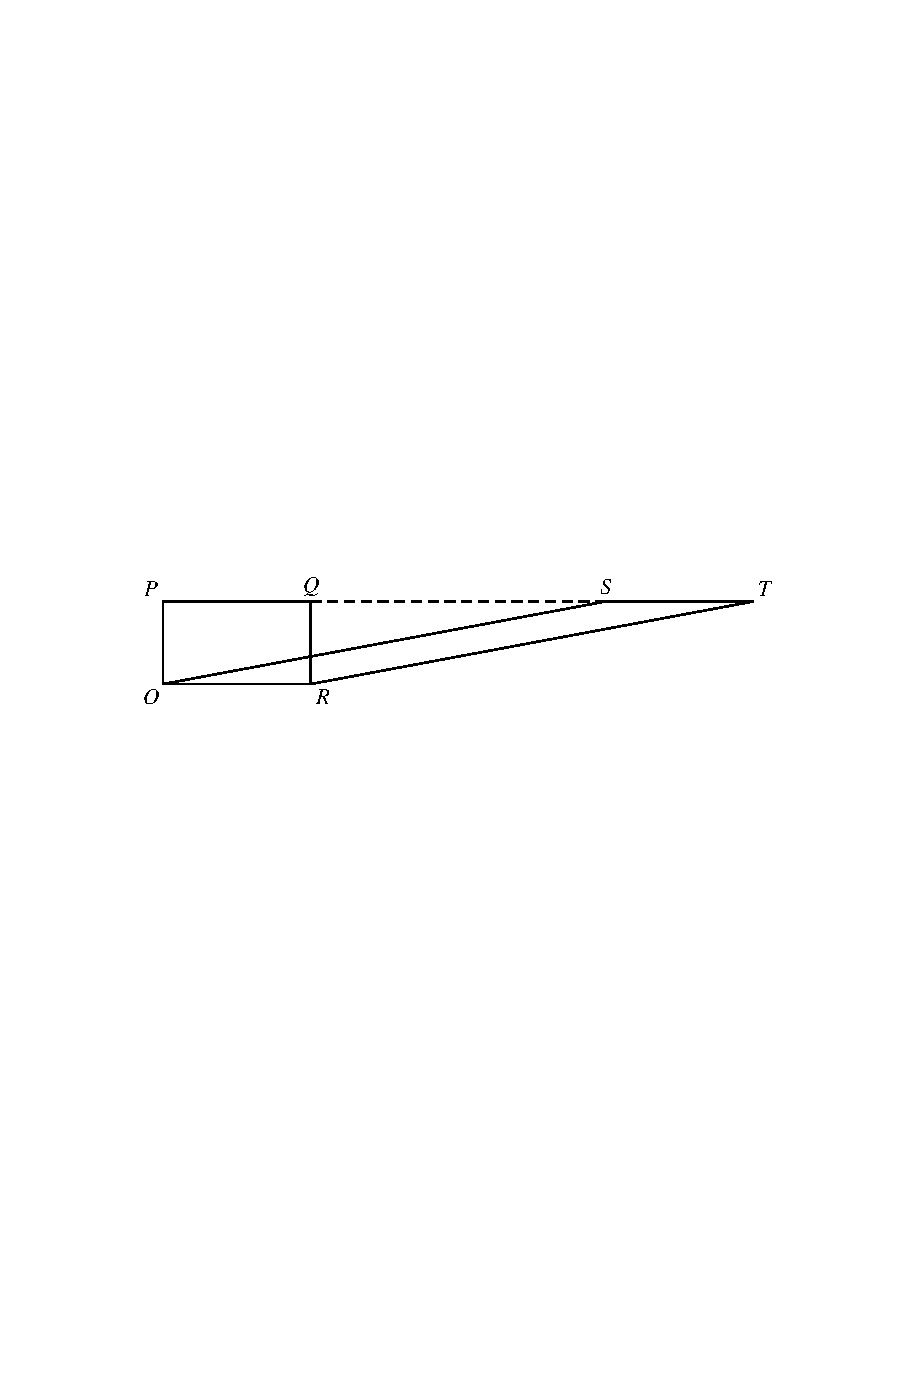
\includegraphics[width=12cm]{BILDER/BildFlaecheParallelogramm2.pdf}}

%% Beweis durch Adition der Flaeche des Dreiecks ORT und Subtraktion
%% der Flaeche des Dreiecks POS

%\centerline{\includegraphics[width=12cm]{BILDER/BildFlaecheParallelogramm3.pdf}}
%\centerline{\includegraphics[width=12cm]{BILDER/BildFlaecheParallelogramm4.pdf}}

Für ein Dreieck folgt entsprechend:
$$
    \mbox{Fläche des Dreiecks} \; = \; \frac{1}{2} \cdot |\mbox{Grundseite}| \cdot |\mbox{Höhe}|
$$

\subsection*{Proportionalitätsprinzip und Anwendungen}

Aus der Formel für die Fläche eines Dreiecks lässt sich ein wichtiges {\em Proportionalitätsprinzip}
ableiten:

%% Das folgende ist Euklid I.37!? bzw. Euklid VI.1

\begin{quote}
    Die Flächen von Dreiecken mit einer gleich langen Grundseite (Höhe) verhalten sich proportional
    zu ihrer Höhe (Grundseite).
\end{quote}

In Euklids Elementen ist die Herleitung dieses Prinzips sehr umständlich, weil ihm ein moderner
Zahlbegriff (insbesondere die reellen Zahlen) fehlten. In Buch V und VI führt er hierfür eine
komplizierte "`Proportionstheorie"' ein.

Interessante Anwendungen des Proportionalitätsprinzips sind einfache Beweise für den Satz des
Pythagoras und für den Strahlensatz. %\ref{thm:strahlensatz}
% Bilder aus Stillwell!! (S.32-33)

%\centerline{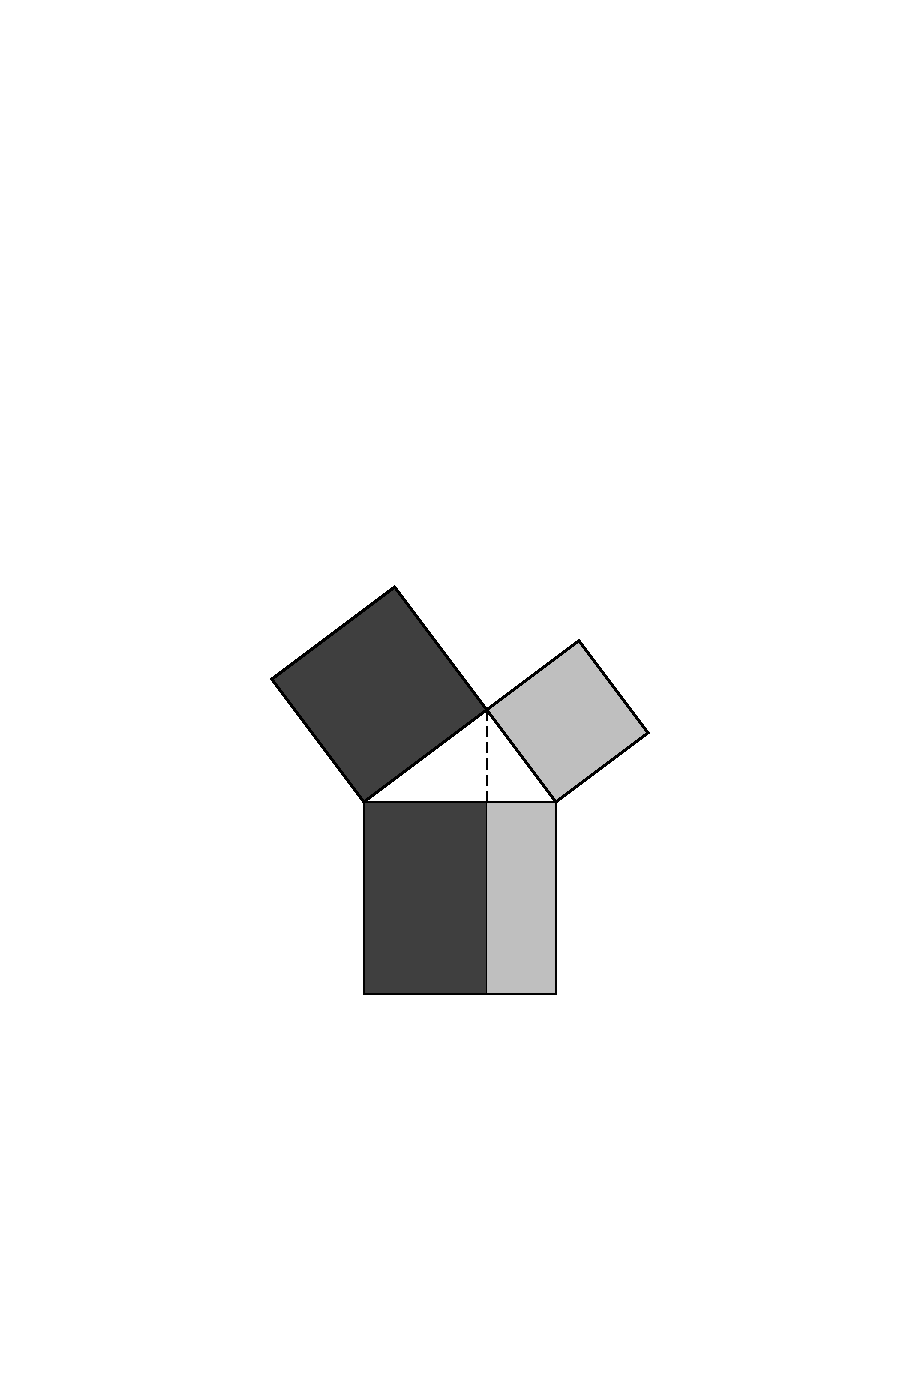
\includegraphics[width=8cm]{BILDER/BildSatzDesPythagoras.pdf}}

\centerline{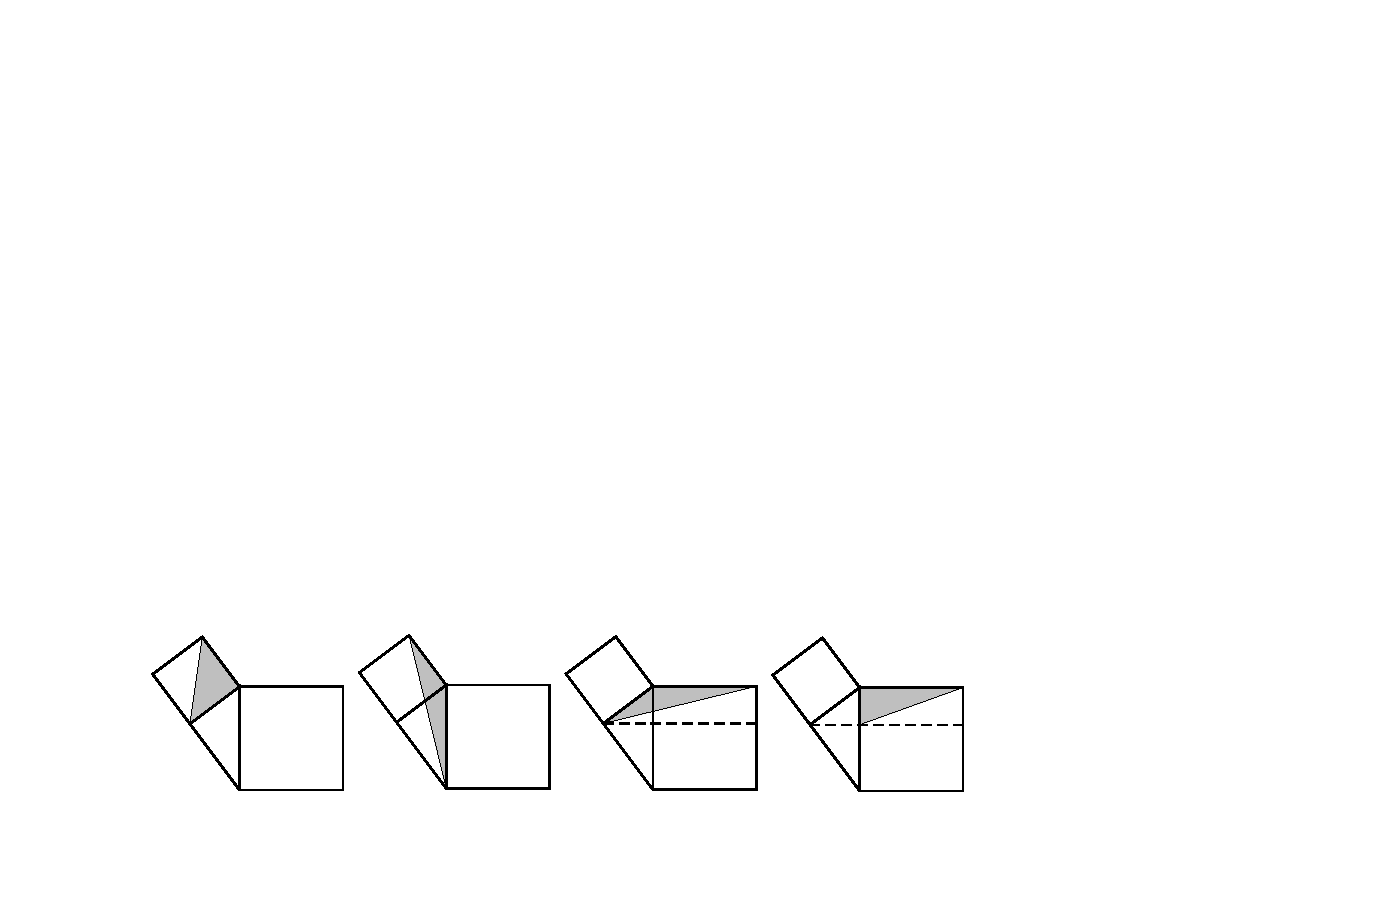
\includegraphics[width=16cm]{BILDER/BildSatzDesPythagoras2.pdf}}

Der im Bild angedeutete Beweis für den Satz von Pythagoras zeigt in drei Schritten, dass der
Flächeninhalt (bzw. der halbe Flächeninhalt) eines kleinen Quadrats gleich dem Flächeninhalt eines
enstprechenden Rechtecks innerhalb des großen Quadrats ist. Dabei wird im ersten und dritten Schritt
das Proportionalitätsprinzip angewendet und im zweiten Schritt das SWS-Kriterium. Diese Beweisidee
geht auf Euklid zurück.

\begin{proof}[Beweis des Strahlensatzes \ref{thm:strahlensatz}]
    Wir betrachten ein Dreieck $ABC$ und Punkte $P,Q$ wie im Satz angegeben. % siehe Bild...

    \begin{center}
        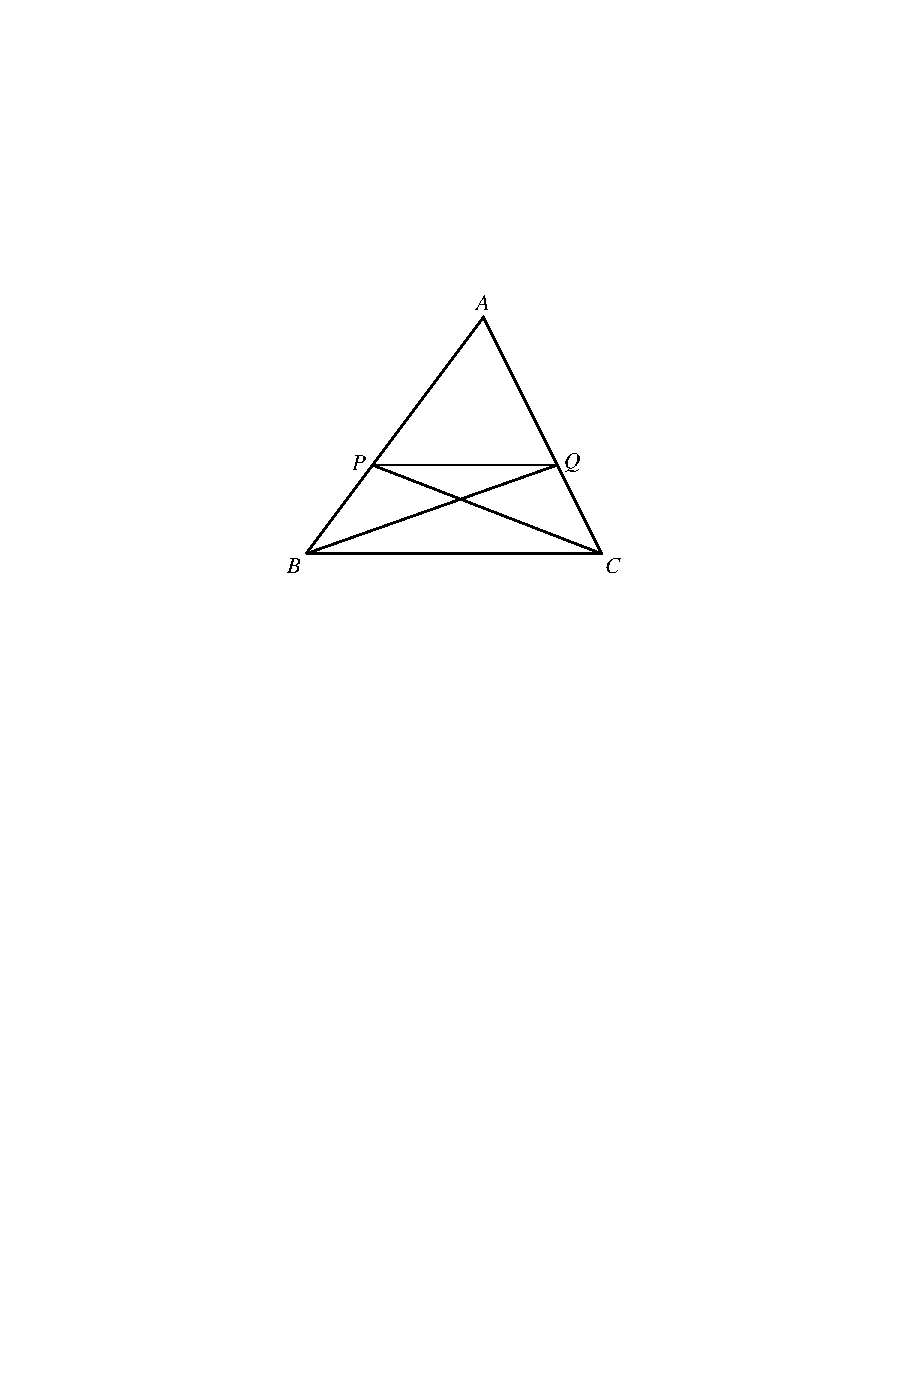
\includegraphics[width=8cm]{BILDER/BildBeweisStrahlensatz.pdf}
    \end{center}

    Weil die Geraden duch $P,Q$ und $B,C$ nach Voraussetzung parallel sind, haben die Dreiecke $PQB$
    und $PQC$ die gleiche Höhe und damit, nach dem Propotionalitätsprinzip, den gleichen
    Flächeninhalt: $|PQB|=|PQC|$. Durch Addition der Fläche des Dreiecks $APQ$ stellen wir fest, das
    die Dreiecke $AQB$ und $APC$ ebenfalls den gleichen Flächeninhalt haben.

    Die Dreiecke $APQ$ und $PQB$ haben die gleiche Höhe in Bezug auf ihre Grundseiten auf der
    Geraden durch $A$ und $B$. D.h., nach dem Propotionalitätsprinzip verhalten sich die Längen der
    Grundseiten zueinander wie ihre Flächeninhalte:
    $$
    \frac{|APQ|}{|AQB|} = \frac{|AP|}{|PQ|}
    $$
    Durch ein analoges Argument für die Dreiecke $PQC$ und $APQ$ erhält man auch
    $$
    \frac{|APQ|}{|PQC|} = \frac{|AQ|}{|QC|}.
    $$
    Wegen $|PQB|=|PQC|$ sind die beiden rechten Seiten gleich, und damit auch die beiden linken
    Seiten.
\end{proof}

{\em Kritik:} Der Beweis des Strahlensatzes verwendet das Proportionalitätsprinzip. Für den Beweis
des Proportionalitätsprinzips benötigt man auch eine Form des Strahlensatzes, so dass es hier in
Euklids Werk zu einem unerlaubten "`Ringschluss "'\ kommt.

% Anmerkung aus Neßelmann-Skript:
%In der Schule wird der Strahlensatz mitunter \"{u}ber Fl\"{a}cheninhalte von
%Dreiecken behandelt, und zwar mit der bekannten Formel
%$F=\frac{1}{2}\cdot g\cdot h$. F\"{u}r den Beweis der Unabh\"{a}ngigkeit der
%Formel von der Auswahl der Grundlinie wird aber gerade der
%Strahlensatz ben\"{o}tigt, wodurch man unwillk\"{u}rlich in einen
%Zirkelschluss ger\"{a}t. Daher f\"{u}hrt dieser Weg zu \underline{keinem}
%Beweis des Strahlensatzes:

%% FOLGENDES AN DEN ANFANG JEDER VORLESUNG (und genauer??)?!?
%\subsection*{Literatur}
%\cite[Kapitel 1 und 2]{SS-2005},
%\cite[Chapter 1]{stillwell-2005},
%\cite[Chapter 1]{hartshorne-2000}
%\cite[Chapter 1]{coxeter-1969}


\chapter{Hilbert}
\section*{Vorlesung am 14.04.2011}

\begin{quote}
    It is quite natural that, after a lapse of about 2250 years, some details are now seen to be
    capable of improvement. (Coxeter, \cite[Section 1.2]{coxeter-1969})
\end{quote}

\subsection*{Hilbert}

\begin{itemize}
    \item In seinem Buch \cite{hilbert} hat David Hilbert (1862--1943) das Axiomensystem von Euklid
        gründlich überarbeitet.

    \item Hilbert verfolgt damit das Ziel, die Axiomatische Geometrie frei von unserer (oft in die
        Irre führenden) geometrischen Anschauung zu machen.

    \item Wir folgen im Wesentlichen der Aufarbeitung~\cite{hartshorne-2000} durch Robin Hartshorne
\end{itemize}

% BEM (taken from Wikipedia, http://en.wikipedia.org/wiki/Hilbert%27s_axioms): Other well-known
% modern axiomatizations of Euclidean geometry are those of Alfred Tarski and of George Birkhoff.

% ETWAS FORMALER:
% Formal "richtig" wäre es eine Menge von Punkten $\P$ einzuführen und eine Menge von Geraden $\MG$
% von Teilmengen von $\P$ (also \MG\subseteq 2^{\P}$. Eine Ebene~$\E$ ist dann ein Tripel $(\P,\MG,
% \MI)$ mit einer Inzidenzrelation $\MI$, die die Axiome I1,I2,I3 erfüllt.

Wir gehen aus von einer nichtleeren Menge~$\E$, deren Elementen wir {\em Punkte} nennen.
(Bezeichnung: $A,\,B,\,C,\ldots$).

{\em Geraden} sind gewisse Teilmengen von $\E$ (Bezeichnung: $g,\,h,\ldots$);

Man beachte, dass wir nicht erklären (können!) "`was Punkte und Geraden sind"'. Wir können aber
durch Axiome angeben welche Eigenschaften Punkte und Geraden haben oder wie sie zueinander in
Beziehung stehen.

% Wir betrachten 5 Gruppen von Axiomen:
% \begin{enumerate}
%     \item[I.] Axiome der Inzidenz
%     \item[II.] Axiome der Anordnung
%     \item[III.] Axiome der Kongruenz
%     \item[IV.] Axiome der Stetigkeit
%     \item[V.] Parallelenaxiom
% \end{enumerate}
% Die Axiome der Axiomengruppen I-IV sind die Axiome der
% "`{}absoluten
% Geometrie"'{}.\\

\subsection*{Inzidenzaxiome}

Wir sagen ein Punkt $A$ {\em inzidiert} mit einer Geraden $g$ genau dann wenn $A$ "`auf $g$ liegt"'
(bzw. $A\in g$).

\begin{itemize}
    \item[{\bf (I1)}] Zu je zwei verschiedenen Punkten $A,\,B\in\E$ gibt es genau eine Gerade
        $g\subset\E$ mit $A,\,B\in g$

    \item[{\bf (I2)}] Auf jeder Geraden gibt es mindestens 2 Punkte.

    \item[{\bf (I3)}] Es gibt 3 Punkte $A,\,B,\,C\in\E$, die nicht auf einer Geraden liegen
\end{itemize}

Die Gerade durch $A$ und $B$ in {\bf(I1)} bezeichnen wir auch mit $g(A,B)$. Drei Punkte $A,\,B,\,C$
heißen \emph{kollinear} wenn sie auf einer gemeinsamen Gerade liegen.  Das Axiom {\bf(I3)} sagt also
aus, dass es 3 nicht kollineare Punkte in $\E$ gibt.

Die Axiome sind {\em unabhängig voneinander}, d.h. eines kann nicht aus den anderen hergeleitet
werden. Für den Beweis der Unabhängigkeit betrachtet man Modelle (Beispiele), in denen alle Axiome
bis auf eins erfüllt sind.

\begin{center}
    % Vorlage:
    %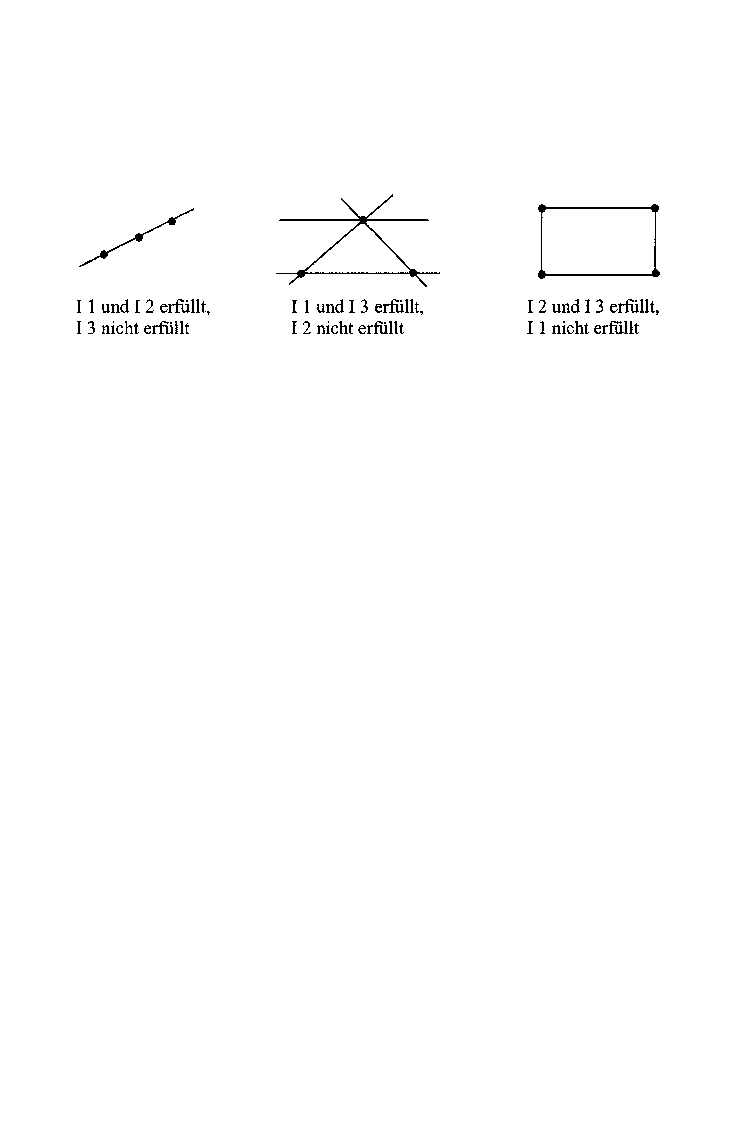
\includegraphics[width=12cm]{BILDER/BildUnabhaengigkeitInzidenzaxiome.pdf}

    % In den .tikz Dateien sind die Zeichnungen für die Bilder. Durch die Tabelle sieht der Abstand
    % zwischen den Bildern schöner aus.
    \begin{figure}[h]
        \begin{tabular}{ccc}
        \begin{tikzpicture}
	\fill [color=colPkt] (0,0) circle (1.5pt);
	\fill [color=colPkt] (1,0.5) circle (1.5pt);
	\fill [color=colPkt] (2,1) circle (1.5pt);
	\draw (-0.5,-0.25) -- (2.5,1.25);
	\draw (1,-0.5) node[anchor=north, text width=3.5cm] {(I1) und (I2) erfüllt, (I3) nicht erfüllt};
\end{tikzpicture}

        &
        \begin{tikzpicture}
	\fill [color=colPkt] (0,0) circle (1.5pt);
	\fill [color=colPkt] (2,0) circle (1.5pt);
	\fill [color=colPkt] (1,1) circle (1.5pt);
	\draw (-0.25,-0.25) -- (1.25,1.25);
	\draw (0.75,1.25) -- (2.25,-0.25);
	\draw (-0.35,0) -- (2.35,0);
	\draw (-0.35,1) -- (2.35,1);
	\draw (1,-0.5) node[anchor=north, text width=3.5cm] {(I1) und (I3) erfüllt, (I2) nicht erfüllt};
\end{tikzpicture}

        &
        \begin{tikzpicture}
	\fill [color=black] (0,0) circle (1.5pt);
	\fill [color=black] (2,0) circle (1.5pt);
	\fill [color=black] (0,1) circle (1.5pt);
	\fill [color=black] (2,1) circle (1.5pt);
	\draw (0,0) -- (2,0) -- (2,1) -- (0,1) -- (0,0);
	\draw (1,-0.5) node[anchor=north, text width=3.5cm] {(I2) und (I3) erfüllt, (I1) nicht erfüllt};
\end{tikzpicture}

        \end{tabular}
        \caption{Unabhängigkeit der Inzidenzaxiome}
    \end{figure}
\end{center}

Eine Menge $\E$ von Punkten, mit einer Menge %$\MG$
von Geraden, die zusammen die Axiome {\bf(I1)}, {\bf(I2)} und {\bf(I3)} erfüllen, heißt auch {\em
Inzidenzgeometrie}. Wir bezeichnen $\E$ in diesem Fall auch als {\em Ebene}.
%Formal ist dies ein Tripel (\E,\MG,\MI) mit
%einer Inzidenzrelation $\MI\subseteq \E |times \MG$.
Auch wenn wir noch nicht viel gefordert haben, lassen sich schon erste einfache Schlußfolgerungen
ziehen, die für alle Inzidenzgeometrien gelten:

\begin{thm}
    Für eine Ebene $\E$, in der die Axiome {\bf(I1)}, {\bf(I2)} und {\bf(I3)} erfüllt sind, gilt:
    \begin{enumerate}
        \item Es gibt mindestens 3 paarweise verschiedene Geraden.

        \item Zwei verschiedene Geraden können höchsten einen gemeinsamen Punkte enthalten.
    \end{enumerate}
\end{thm}

\begin{proof}
    \begin{enumerate}
    \item[(2)] Enthalten zwei unterschiedliche Geraden $g$ und $h$ zwei unterschiedliche
        Schnittpunkte $A$ und $B$, so widerspricht das Axiom {\bf(I1)}, in der die Eindeutigkeit der
        Geraden durch $A$ und $B$ gefordert wird.

    \item[(1)] Nach Axiom {\bf(I3)} gibt es drei Punkte die nicht kollinear sind. Die Geraden
        $g(A,B), g(A,C)$ und $g(B,C)$ sind wiederum paarweise verschieden nach {\bf(I1)}.
    \end{enumerate}
\end{proof}

Man beachte, dass die Argumentation im Beweis unabhängig von unserer "`geometrischen Anschauung"'
ist. Wir können sogar {\em Modelle} angeben, die weit entfernt sind von unserer geometrischen
Anschauung einer Ebene, die aber trotzdem die Inzidenzaxiome erfüllen. Wir betrachten ein paar
Beispiele:

\begin{description}
    \item[Modell 1] $\E=\{A,\,B,\,C\}$ - 3 paarweise verschiedene Punkte;\\
        Geraden: mögliche Tupel $\{A,\,B\},\;\{A,\,C\},\;\{B,\,C\}$
        % Das kleinstmögliche Modell

    \item[Modell 2] \label{Modell2} $\E=\{A,\,B,\,C,\,D\}$ - 4 paarweise verschiedene Punkte;\\
        Geraden: mögliche Tupel $\{A,\,B\},\; \{A,\,C\},\; \{A,\,D\},\; \{B,\,C\},\; \{B,\,D\},\;
        \{C,\,D\}$
        % Das kleinst mögliche Modell einer affinen Inzidenzgeometrie
\end{description}

Ist $\E$ endlich so spricht man auch von einer {\em endlichen Geometrie}.  Solche Geometrien werden
in der {\em Kombinatorik} untersucht.

\begin{description}
    \item[Modell 3] $\E=\R^2$ und Geraden "`wie üblich"' als Lösungen linearer Gleichungen
        $a x + b y = c$ mit $a,b,c\in \R$ ($a,b$ nicht beide $0$).
        % Hier als Beispiel auch über anderen Körpern?!
        % Dann ist Modell 2 Spezialfall für $K=F_2$!

    \item[Modell 4] ("`Bierdeckelgeometrie"')\\ % nach Felix Klein
        $\E=\{ (x,y)\in\R^2 | x^2+y^2<1 \}$; Geraden sind die Geraden aus Modell 3 geschnitten mit
        $\E$

    \item[Modell 5] ("`Halbebenenmodell von Poincaré"')\\
        $\E=\{ (x,y)\in\R^2 | y>0 \}$; Geraden sind entweder Halbkreise oberhalb der $x$-Achse oder
        Halbgeraden Senkrecht zur $x$-Achse. Das rechte Bild zeigt wie die Gerade zu zwei
        verschiedenen Punkten konstruiert wird.

    \item[Modell 6] ("`Sphärisches Modell der projektiven Ebene"')\\
        $\E=\{ (x,-x)\in\R^{3+3} \ | \ x_1^2+  x_2^2 + x_3^2= 1 \}$, d.h., Punkte sind in diesem
        Modell Paare von diametral liegenden Vektoren auf der Einheitssphäre; Geraden sind
        Punktmengen die auf einem Großkreis (Schnitt der Sphäre mit einer $2$-dimensionalen Ebene
        durch den Ursprung) liegen.
\end{description}

\begin{figure}[h]
    % Erzeugt mit GeoGebra aus ./ggb/Bierdeckelgeometrie.ggb mit
% xmin = -0.5
% ymin = -0.5
% xmax =  4.5
% ymax =  4.5
\begin{tikzpicture}[line cap=round,line join=round,>=triangle 45,x=1.0cm,y=1.0cm]
    \clip(-0.5,-0.5) rectangle (4.5,4.5);
    \draw(2,2) circle (2cm);
    \draw (0.59,0.59)-- (3.41,0.59);
    \draw (0.26,2.99)-- (3.74,1.01);
    \draw (0.02,2.31)-- (3.03,3.72);
    \draw (1.14,3.81)-- (3.87,1.29);
    \fill [color=colPkt] (1.41,2.34) circle (1.5pt);
    \fill [color=colPkt] (1.84,3.16) circle (1.5pt);
    \fill [color=colPkt] (1.54,3.44) circle (1.5pt);
    \fill [color=colPkt] (2.58,3.51) circle (1.5pt);
    \fill [color=colPkt] (2.78,2.3) circle (1.5pt);
\end{tikzpicture}

    \caption{"`Bierdeckelgeometrie"'}
\end{figure}

\begin{figure}[h]
    \begin{tabular}{cc}
        % Konzipiert mit GeoGebra aus ./tikz/HalbebenenmodellPoincare.tikz
% Der TikZ Output ist aber Mist, daher wurde hier selbst Hand angelegt.
\begin{tikzpicture}[]
    % beschränkt das gesamte Bild auf das angegebene Rechteck:
    \clip (-2.5,-0.5) rectangle (5.5,3);
    % Jetzt folgen die drei Halbkreise. Es sind eigenlich normale Kreise, die aber vorher geclippt,
    % also beschnitten werden (anders geht's nicht).
    \begin{scope}
        % Eigentlich müsste man nur von (1.5,0) bis (3.5,1.0) beschränken, da sich der Halbkreis
        % nur in diesem Bereich befindet, aber dann sieht's an den Grenzen doof aus (am besten
        % selbst ausprobieren und anschauen):
        \clip (1.4,0) rectangle (3.6,1.1);
        % Der Kreis an sich ist straightforward:
        \draw (2.5,0) circle (1cm);
    \end{scope}
    % Die restlichen beiden Halbkreise:
    \begin{scope}
        \clip (-1.1,0) rectangle (4.1,2.6);
        \draw (1.5,0) circle (2.5cm);
    \end{scope}
    \begin{scope}
        \clip (-2.1,0) rectangle (2.1,1.6);
        \draw (-0.5,0) circle (1.5cm);
    \end{scope}
    % Die Gerade ganz rechts und die beiden Achsen. Die Gerade hat im Gegensatz zum Originalbild
    % keinen Pfeil, weil sie meiner Meinung nach kein Strahl ist.
    \draw (5,0) -- (5,3);
    \draw [->] (0,0) -- (0,3);
    \draw [->] (-2.5,0) -- (5.5,0);
\end{tikzpicture}

        &
        % Auch hier hat GeoGebra den TikZ-Output versaut, daher wird's selbst zurechtgebogen. Oder gleich
% ganz selbstgemacht.
\begin{tikzpicture}[]
    % Beschränkung für das gesamte Bild, eigentlich nicht notwendig, erzeugt aber überall 0.5cm
    % Abstand, was ganz brauchbar ist.
    \clip (-0.5,-0.5) rectangle (5,2.5);
    % x-Achse:
    \draw [->] (0,0) -- (5,0);
    % Ursprung des Koordinatensystems:
    \coordinate (U) at (2.5,0);
    \fill [color=colPktKon] (U) circle (2pt);
    % der Halbkreis:
    \begin{scope}
        \clip (0.4,0) rectangle (4.6,2.1);
        % Ganz schöne Verrenkung:
        % Da wir den Kreis gleich nochmal für die Punkte auf dem Kreis brauchen, geben wir ihm mit
        % \node den Namen (c). Dadurch wird das Zeichnen aber komisch. Zum Verständnis einfach mal
        % den Kram in den eckigen Klammern ausblenden und schauen was dasteht: wir definieren eine
        % Node mit dem Namen (c) an Koordinate (2.5,0). Soweit so gut. Diese Node soll gezeichnet
        % werden (draw), soll ein Kreis sein (circle) und eine minimale Größe von 4cm haben, was
        % hier dem Durchmesser entspricht.
        \node [draw, circle, minimum size=4cm] (c) at (U) {};
    \end{scope}
    % Punkt A soll auf dem Kreis liegen und die x-Koordinate soll 1 sein. Dafür soll uns TikZ den
    % Schnittpunkt aus dem Kreis und der Strecke (1,0) -- (1,2) berechnen:
    \coordinate [label=130:$A$] (A) at (intersection of (1,0) -- (1,2) and c);
    % und jetzt muss Punkt A nur noch gezeichnet werden:
    \fill [color=colPkt] (A) circle (2pt);
    % bei Punkt B verfahren wir genauso, außer dass wir dafür die Strecke für den Schnittpunkt auch
    % noch zeichnen müssen (keine Ahnung warum, aber ohne gibt's nicht den richtigen Schnittpunkt)
    \path (4.3,0) -- (4.3,2);
    \coordinate [label=right:$B$] (B) at (intersection of (4.3,0) -- (4.3,2) and c);
    \fill [color=colPkt] (B) circle (2pt);
    % Strecke zwischen A und B:
    \draw (A) -- (B);
    % Mittelpunkt zwischen AB:
    \node (X) at ($ (A)!.5!(B) $) {};
    % Strecke vom Ursprung zum Mittelpunkt
    % Keine Ahnung, warum man nicht einfach (U) -- (X) machen kann, er macht's nicht richtig. Wenn
    % man aber sagt, er soll es genau bis (X) machen, dann wird's auch richtig gezeichnet. Komisches
    % Ding.
    \draw (U) -- ($ (U)!1.0!(X) $);
    %TODO: folgenden Kram erklären!
    \draw ($ (X)!0.3!(A) $) let
            \p1 = ($ (X) - (A) $)
        in
            arc (170:257:{0.3*veclen(\x1,\y1)});
    \fill let
            \p1 = ($ (X)!0.13!(A) $), \p2 = ($ (X)!0.1!(U) $)
        in
            (\x1,\y2) circle (1pt);
\end{tikzpicture}

    \end{tabular}
    \caption{Halbebenenmodell von Poincaré}
\end{figure}

% Folgendes kann man vielleicht mit sphärischer Geometrie, d.h. mit
% Geometrie auf der Oberfläche einer Kugel motivieren... Man beachte
% allerdings, dass für diametral liegende Punkte auf der Sphäre keine
% eindeutige Gerade (Großkreis) existiert => (I1) ist verletzt!

In einer Inzidenzgeometrie kann man bereits Parallelen einführen.

\begin{defi}[Parallelität]
    Zwei Geraden $g,\,h \subset \E$ heißen {\em parallel} (in Zeichen $g\|h$) wenn sie gleich sind
    oder einen leeren Schnitt haben.
    %($g\|h$) $:\Longleftrightarrow$ entweder $g\cap h=\emptyset$ oder $g=h$.}
\end{defi}

Die Existenz von Parallelen kann nicht aus den Inzidenzaxiomen hergeleitet werden! In Modell 1 gibt
es keine Parallelen. In Modell 4 gibt es zu jeder Geraden unendlich viele Parallelen!

% An dieser Stelle schon das Parallelenaxiom angeben??
% Nach folgender Definition 

%\begin{enumerate}
%\item[{\bf(P)}]
%Sei $g\subset \E$ eine Gerade und $P\in \E$ ein Punkt. Dann gibt es
%höchstens eine Gerade $h\subset \E$
%die $P$ enthält und parallel zu $g$ ist.
%\end{enumerate}

Eine Ebene $\E$ die die 3 Axiome der Inzidenzgeometrie erfüllt und zusätzlich das Parallelenaxiom
heißt auch {\em affine Inzidenzgeometrie}. Modell 2 und Modell 4 sind Beispiele. Es ist ein
schwieriges (und noch offenes) Problem die endlichen, affinen Inzidenzgeometrien zu klassifizieren.

% UEBUNG: (??)
% Man kann zeigen, dass jede Gerade einer endlichen affinen Inzidenzgeometrie die gleiche Anzahl von
% Punkten hat (wie?).  Diese Anzahl q wird ueblicherweise die Ordnung der Ebene genannt.  Man kann
% ferner zeigen, dass die Ebene der Ordnung q, q+1 Geraden durch jeden Punkt, und insgesamt q^2
% Punkte und q^2+q Geraden besitzt.

% Affine Ebenen der Ordnung $n$ gibt es immer, wenn n eine Primzahlpotenz ist.
% Für $n=10$ wurde die Nichtexistenz mittels Computer-assisted-proof bewiesen:
% Lam, C. W. H. (1991), "The Search for a Finite Projective Plane of Order 10", American
% Mathematical Monthly 98 (4): 305318
%
% Es ist offen, ob es eine affine / projektive Ebene der Ordnung
% $n = 12$ gibt!?
%
% SEE ALSO: http://de.wikipedia.org/wiki/Affine_Ebene

\section*{Vorlesung am 19.04.2011}

\subsection*{Axiome der Anordnung}

% Historische Bemerkung zu einem Zitat von Gauß, der erkannt hatte, dass man die Relation "Zwischen"
% vernünftig erklären muss?

%% INTERESSANTER HINTERGRUND:
% In Hilbert's Buch (1 Ausgabe von 1899 / siehe auch die Englische Übersetzung) gibt es noch ein
% weiteres Axiom der Anordnung, von dem aber "R. L. Moore proved that this axiom is redundant, in
% 1902". see http://en.wikipedia.org/wiki/Hilbert%27s_axioms In der 2. Auflage von 1903 ist dieses
% Axiom nicht mehr angeführt.  In beiden Ausgaben ist aber die Rede davon, dass es einfach sei die
% Unabhängigkeit der Axiome voneinander zu beweisen!!!! :-) (siehe Anfang von §10)

Wir gehen im Folgenden davon aus, dass $\E$ eine Ebene ist, die die 3 Axiome der Inzidenzgeometrie
erfüllt. Wir wollen schrittweise Axiome hinzufügen, die uns näher an die Geometrie Euklids
heranbringen.  Wir werden dabei zunächst (so lange wie möglich) auf das Parallelenaxiom verzichten.

In Euklids Elementen haben wir gesehen, dass häufig Begriffe der Anordnung benutzt werden. Zum
Beispiel: "`ein Punkt %$C$
liegt {\em zwischen} zwei anderen Punkten %$A$ und $B$ 
%% Vergleiche auch den Beweis von "Alle Dreiecke sind gleichschenklig"
auf einer Geraden"' .
Oder: "`Ein Punkt %$A$
liegt {\em auf der anderen Seite} einer Geraden"'. Konzepte wie "`{\em Innen}"' und "`{\em
Außen}"' oder "`Größenvergleiche"' von Strecken und Winkeln hängen damit zusammen. Die folgenden
Axiome der Anordnung dienen der Präzisierung dieser Begriffe.

Die Punkte einer jeden Geraden $g$ von $\E$ stehen in einer Beziehung zueinander, die "`Zwischen"'
heißt und folgenden Bedingungen genügt:

\begin{enumerate}
    \item[{\bf (A1)}] Wenn $A,\,B,\,C$ auf einer Geraden $g$ liegen und $B$ zwischen $A$ und $C$
        liegt (in Zeichen: $\Zw(ABC)$), dann sind $A,\,B,\,C$ paarweise verschieden und $B$ liegt
        auch zwischen $C$ und $A$ ($\Zw(CBA)$).

    \item[{\bf (A2)}] Zu je zwei verschiedenen Punkten $A,\,B$ gibt es einen Punkt $C$, so dass
        $\Zw(ABC)$.

    \item[{\bf (A3)}] Zu je 3 verschiedenen Punkten auf einer Geraden $g$ gibt es genau einen, der
        zwischen den anderen beiden liegt.
\end{enumerate}

% BEM: (Es ist ausreichend: "`höchstens"' einen zu fordern!)
% Beweis?!?!?

Auf Basis der Beziehung "`Zwischen"' können wir präzisieren was eine Strecke ist:

\begin{defi}[Strecke]
    Seien $A,\,B\in \E$ zwei verschiedene Punkte. Dann heißt die Menge

    $$
    \str{AB}:=\{A,\,B\}\cup\{X\in\E \; | \;\Zw(AXB)\}
    $$

    die {\em Strecke} $\str{AB}$ oder auch $\str{BA}$. $A$ und $B$ sind {\em Randpunkte}, $\{X \in
    \varepsilon:\; \Zw(AXB)\}$ sind {\em innere Punkte} der Strecke.
\end{defi}

Eine Gerade $g$ \emph{schneidet} eine Strecke $\str{AB}$, wenn $g\cap\str{AB}\neq \emptyset$.

Um etwa die Teilung einer Ebene durch eine Gerade in zwei disjunkte Teilmengen
%und das Prinzip "`{}Ebene"'{}   %% WAS IST DAMIT GEMEINT?!?
zu erklären, benötigt man ein weiteres Axiom:

%% ACHTUNG: Die Teilung der Ebene in zwei Hälften ist als Axiom irgendwie einfacher (??), und das
%% Axiom von Pasch ist dazu äquivalent.  Beim nächsten Mal sollte man daher vielleicht eher das
%% "Theorem über die Teilung der Ebene" siehe

\begin{enumerate}
    % Pasch hat dieses Axiom 1882 formuliert
    \item[{\bf (A4)}] {\bf (Axiom von Pasch)} Seien $A,\,B,\,C\in\E$ nicht kollinear und
        $g\subset\E$ eine Gerade mit $A,\,B,\,C\notin g$. Wenn $g$ die Strecke $\str{AB}$ schneidet,
        so schneidet $g$ auch die Strecke $\str{AC}$ oder $\str{BC}$, aber nicht beide.
    % (Letzteres ist auch beweisbar!)
    % WIE ?!?!
\end{enumerate}

% AUS WIKIPEDIA:
% Anschaulich gesprochen: "Wenn eine Gerade durch eine Seite ins Innere eines Dreiecks eintritt, so
% tritt sie gewiss auch wieder durch eine Seite des Dreiecks heraus.
% AN DIESER STELLE FEHLT UNS ALLERDINGS DER BEGRIFF "Inneres eines Dreiecks"!!!?

\begin{figure}[h]
    \begin{tikzpicture}[line cap=round,line join=round,>=triangle 45,x=1.0cm,y=1.0cm]
    \clip(-0.5,-0.5) rectangle (4.5,2.5);
    \draw (3,2) coordinate (A);
    \draw (0,0) coordinate (B);
    \draw (4,0) coordinate (C);
    \draw (A)--(B)--(C)--(A);
    \draw [domain=-0.5:4.5] plot(\x,{(--19-7*\x)/10});
    \filldraw [color=colPkt] (A) circle (1.5pt) node[above] {$A$};
    \filldraw [color=colPkt] (B) circle (1.5pt) node[left]  {$B$};
    \filldraw [color=colPkt] (C) circle (1.5pt) node[right] {$C$};
    \draw[color=black] (B) node[above=1.2cm] {$g$};
\end{tikzpicture}

    \caption{Axiom von Pasch}
\end{figure}

% In den folgenden Sätzen seien die Axiome der Inzidenz und der Anordnung für die betrachtete Ebene
% $\E$ erfüllt.

\begin{thm}
    Erfüllt eine Ebene $\E$ die Axiome der Inzidenz und der Anordnung, so hat jede Strecke
    mindestens einen inneren Punkt und damit unendlich viele.
\end{thm}

\begin{proof}
    Sei $\str{AB}$ gegeben.
    \begin{align*}
        \stackrel{(I3)}{\Longrightarrow}\ & \exists\,E\notin g(A,B)\\
        \stackrel{(A2)}{\Longrightarrow}\ & \exists\,F\in g(A,E):\;\Zw(AEF)\\
        \stackrel{(A2)}{\Longrightarrow}\ & \exists\,D\in g(F,B):\;\Zw(FBD).\\
        \intertext{Wegen $E\neq F$ und $g(E,D)\neq g(F,D)$ schneidet $g(E,D)$ nicht $\str{FB}$}
        \stackrel{(A4)}{\Longrightarrow}\ & g(E,D) \text{ schneidet } \str{AB} \text{ (im Innern, da
        $A,B$ nach Konstruktion nicht auf der Geraden liegen). }
    \end{align*}

    \begin{figure}[h]
        \begin{tikzpicture}[line cap=round,line join=round,>=triangle 45,x=1.0cm,y=1.0cm]
    \clip(-0.5,-1) rectangle (5.5,2.5);
    \draw (0,0) coordinate (A);
    \draw (4,0) coordinate (B);
    \draw (5,-0.66) coordinate (D);
    \draw (0.6,1.21) coordinate (E);
    \draw (1,2) coordinate (F);
    \draw [domain=-0.5:5.5] plot(\x,{(-0--2*\x)/1});
    \draw [domain=-0.5:5.5] plot(\x,{(--8-2*\x)/3});
    \draw [domain=-0.5:5.5] plot(\x,{(-0-0*\x)/4});
    \draw [dash pattern=on 4pt off 4pt,domain=-0.5:5.5] plot(\x,{(--6.44-1.87*\x)/4.39});
    \filldraw [color=colPkt] (A) circle (1.5pt) node[below] {$A$};
    \filldraw [color=colPkt] (4,0) circle (1.5pt) node[above] {$B$};
    \filldraw [color=colPktKon] (1,2) circle (1.5pt) node[right] {$F$};
    \filldraw [color=colPktKon] (0.6,1.21) circle (1.5pt) node[below] {$E$};
    \filldraw [color=colPktKon] (5,-0.66) circle (1.5pt) node[above] {$D$};
\end{tikzpicture}

        \caption{innerer Punkt einer Strecke}
    \end{figure}
\end{proof}

%% ACHTUNG:
% Oft (?) wird die folgende Teilung der Ebene als Axiom vorausgesetzt und dann erhält man das Axiom
% von Pasch als Satz!!!
%% siehe "Leitfaden Geometrie", S.82 für einen Beweis
% Übung, Blatt 3!!

\begin{thm}[Teilung der Ebene]\label{thm:satz.s1a}
    Sei $\E$ eine Ebene, die die Axiome der Inzidenz und der Anordnung erfüllt, und sei $g \subset
    \E$ eine Gerade. Dann gibt es eine disjunkte Aufteilung der Ebene in nichtleere Teilmengen $g,
    S_1$, und $S_2$ für die gilt:

    \renewcommand{\labelenumi}{\alph{enumi})} % ändert die Nummerierung von (1) auf a)
    \begin{enumerate}
        \item $A,\, B \notin g$ gehören derselben Menge ($S_1$ oder $S_2$) an
            $\Longleftrightarrow\; \str{AB} \cap g = \emptyset$;

        \item $A,\, C \notin g$ gehören zu verschiedenen Mengen $\Longleftrightarrow\;
            \str{AC} \cap g \neq \emptyset$.
    \end{enumerate}
\end{thm}

$S_1$ und $S_2$ heißen die beiden \emph{(verschiedenen) Seiten} von $g$. D.h., $A$ und $B$
liegen auf derselben Seite und $A$ und $C$ auf verschiedenen Seiten von $g$.

\centerline{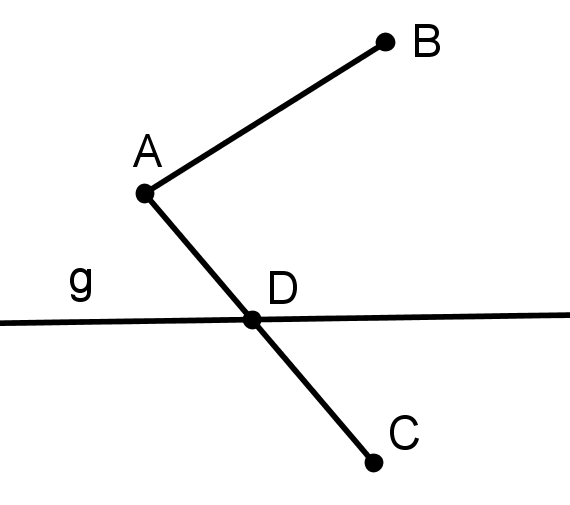
\includegraphics[width=6cm]{BILDER/1-1-06a-Seiten.png}}

Formal definiert jede Gerade $g$ eine Relation auf $\E\setminus g$ durch

$$
    \mbox{Für } A,\, B \in \E \setminus g \mbox{ gilt } A \stackrel{g}{\sim} B :
    \Longleftrightarrow\; A=B\; \mbox{oder}\; A \neq B\; \mbox{und}\; \str{AB} \cap g = \emptyset.
$$

\begin{proof}[Beweis von Theorem \ref{thm:satz.s1a}]
    Zum Beweis des Theorems genügt es zu zeigen, dass $\stackrel{g}{\sim}$ eine Äquivalenzrelation
    mit genau 2 Äquivalenzklassen ist.

    Offenbar ist die Relation reflexiv und symmetrisch: $\forall\, A,\, B \in \E \setminus g : \; A
    \stackrel{g}{\sim} A$ und $\{A \stackrel{g}{\sim} B\; \Rightarrow\; B \stackrel{g}{\sim} A\}$.

    \begin{itemize}
        \item Aufwändiger ist die {\bf Transitivität}:\\
        Sei $A,\, B,\, C \in \E \setminus g$, dann müssen wir zeigen:

        $$
            A \stackrel{g}{\sim} B\; \mbox{ und } B \stackrel{g}{\sim} C\; \Rightarrow\; A
            \stackrel{g}{\sim} C
        $$

        Sei also $\str{AB} \cap g = \emptyset,\; \str{BC} \cap g = \emptyset$.

        \begin{description}
            \item[Fall 1] $A,\, B,\, C$ nicht kollinear

                Falls $\str{AC} \cap g \neq \emptyset\; \stackrel{(A4)}{\Longrightarrow}\; g$
                schneidet weitere Seite $\str{AB}$ oder $\str{BC}$ (im Widerspruch zur
                Voraussetzung).

            \item[Fall 2] $A,\, B,\, C$ kollinear, $C \in h = g(A,B)$.

                Sei $D \in g,\; D \notin h\; \stackrel{(A2)}{\Longrightarrow}\; \exists\, E \in
                g(A,D)$ mit $\Zw(DAE)\; \Rightarrow\; \str{AE} \cap g = \emptyset\; \Rightarrow\; A
                \stackrel{g}{\sim} E.$

                % Wenig hilfreiches Bild: (?!?)
                %\includegraphics[width=3.5cm]{1-1-06b-Seiten}

                % ACHTUNG:
                % Geht dieser Fall nicht viel einfacher zu klären unter Anwendung des folgenden
                % Zusammenhangs:  (den man dann vielleicht auch noch beweisen sollte!!!??? Übung!):
                % Sind $A,B,C$ drei Punkte auf einer Geraden mit $\Zw(ACB)$, so gilt
                % $$
                %   AC \cup CB = AB \quad \mbox{und} \quad AC \cap CB = \{C\}
                % $$

                Nun wenden wir mehrfach Fall 1 an, da  $E,\,A,\,B$ und  $E,\,A,\,C$ nicht kollinear:

                \centerline{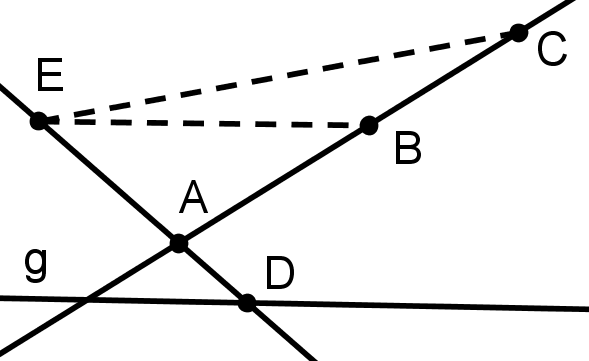
\includegraphics[width=6cm]{BILDER/1-1-06c-Seiten.png}}

                $\str{AE} \cap g = \emptyset,\; \str{AB} \cap g=\emptyset\;
                \stackrel{(A4)}{\Longrightarrow}\; \str{EB} \cap g = \emptyset;\; \str{BC}\cap g =
                \emptyset\; \stackrel{(A4)}{\Longrightarrow}\; \str{EC} \cap g = \emptyset;\;
                \stackrel{(A4)}{\Longrightarrow}\; \str{AC} \cap g = \emptyset$, d.h.
                $A\stackrel{g}{\sim} C$.
        \end{description}

        \item Wir müssen nun noch zeigen, dass es {\bf genau 2 Äquivalenzklassen} gibt.
        \begin{description}
            \item[1. Klasse $S_1$] Wegen \textbf{(I3)} gibt es ein $A \in \E \setminus g$. $S_1$
                können wir daher wählen als

                $$
                    [A] := \{ A \} \cup \{ X \in \E:\, \str{AX} \cap g = \emptyset \}
                $$

            \item[2. Klasse $S_2$] Sei $D\in g$ wie oben

                $$
                    \stackrel{(A4)}{\Longrightarrow} \exists\, C \in \E:\; \Zw(ADC)\; \Rightarrow\;
                    C \notin S_1\; \Rightarrow\; S_2 := [C]
                $$

                \centerline{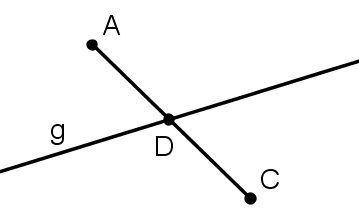
\includegraphics[width=6cm]{BILDER/1-1-06d-Seiten.png}}
        \end{description}

        \item Bleibt zu zeigen, dass es keine weiteren Klassen gibt.\\
            D.h., für $B$ mit $B \stackrel{g}{\nsim} C$ ($B \notin S_2$) sollte $B
            \stackrel{g}{\sim} A$ ($B \in S_1$) folgen.

            % SATZ VON NESSELMANN: (finde ich unverständlich)
            % Sei etwa $B$ derart, dass $B\stackrel{g}{\nsim} C$, d.h. $B\notin S_2$,
            % $\stackrel{Beh.}{\Longrightarrow}\;B\stackrel{g}{\sim} A$, d.h. $B\in S_1$.

        \begin{description}
            \item[Fall 1] $A,\,B,\,C$ nicht kollinear\\
                $\str{AC} \cap g \neq \emptyset,\; \str{BC} \cap g \neq \emptyset\;
                \stackrel{(A4)}{\Longrightarrow}\; \str{AB} \cap g = \emptyset$ d.h. $A
                \stackrel{g}{\sim} B$.

                \centerline{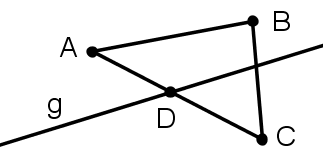
\includegraphics[width=6cm]{BILDER/1-1-06e-Seiten.png}}

            \item[Fall 2] $A,\, B,\, C$ kollinear, $C \in h = g(A,B)$; wie oben $\exists\; D \in
                g,\; D \notin h$ und $E \in g(D,A)$ mit $\Zw(DAE)\; \Rightarrow\; \str{AE} \cap g =
                \emptyset\; (A \stackrel{g}{\sim} E)$\\ $\Longrightarrow\; ({\scriptstyle (A4)\;
                \mbox{\footnotesize für}\; EAC}) \quad \str{EC} \cap g \neq \emptyset.$

                \centerline{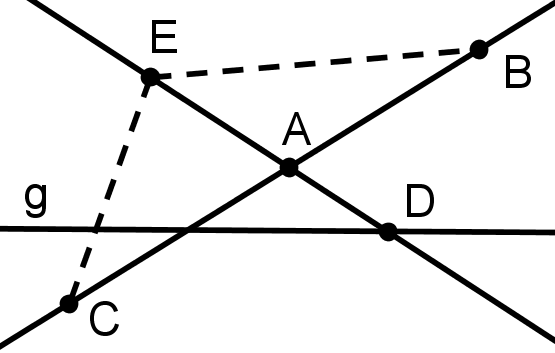
\includegraphics[width=6cm]{BILDER/1-1-06f-Seiten.png}}

                Für die Punkte $E, B, C$ gilt nach Voraussetzung $\str{BC} \cap g \neq \emptyset$.
                Daher ist ebenfalls nach \textbf{(A4)} für Punkte $E, A, B$: $\str{BE} \cap g =
                \emptyset \; \stackrel{(A4)}{\Longrightarrow}\; \str{AB} \cap g = \emptyset$, also
                $B \stackrel{g}{\sim} A$
        \end{description}
    \end{itemize}
\end{proof}

%% ACHTUNG:
% Es fehlt eine Diskussion über die Unabhängigkeit der Anordnungsaxiom!! (angeblich einfach nach
% Hilbert, aber selbst hat er in der 1. Auflage auch einen Fehler gemacht!!!)

\subsection*{Winkel, Strahlen, Dreiecke}

Mit der Aufteilung der Ebene in zwei disjunkte Seiten kann man auch zeigen, dass ein Punkt eine
Gerade in zwei disjunkte Teile zerlegt.

\begin{thm}[Teilung von Geraden]\label{thm:satz.s1b}
    Sei $\E$ eine Ebene, die die Axiome der Inzidenz und der Anordnung erfüllt. Sei $A$ ein Punkt
    auf einer Geraden $g \subset \E$. Dann gibt es eine disjunkte Aufteilung der Geraden $g$ in
    nichtleere Teilmengen $\{A\}, S_1, S_2$ (in {\em Seiten} $S_1$ und $S_2$ bezüglich $A$ mit $g
    \setminus \{A\} = S_1 \cup S_2,\; S_1 \cap S_2 = \emptyset$) für die gilt:
    \renewcommand{\labelenumi}{\alph{enumi})} % ändert die Nummerierung von (1) auf a)
    \begin{enumerate}
        \item $B,\, C \in g$ auf "`derselben Seite"' $\Longleftrightarrow\; B = C$ oder $A \notin
            \str{BC}$;

        \item $B,\, C \in g$ auf "`verschiedenen Seiten"' $\Longleftrightarrow\; A \in \str{BC}$;
    \end{enumerate}
\end{thm}
%\ref{satz.s1b}

\begin{proof}
    Sei $E \notin g$ und $h = g(A,E)$. Dann teilt $h$ gemäß Theorem \ref{thm:satz.s1a} die Ebene in
    2 disjunkte Teilmengen $S_1'$ und $S_2'$. Die Mengen $S_1 = S_1'\cap g$ und $S_2 = S_2' \cap g$
    erfüllen die Bedingungen des Theorems.

    \centerline{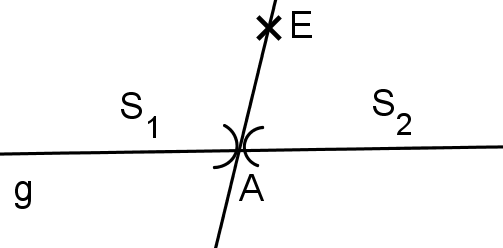
\includegraphics[width=5cm]{BILDER/1-1-07-Satz.png}}
\end{proof}

\section*{Vorlesung am 21.04.2011}

Mit der Aufteilung einer Ebene bzw. einer Geraden in 2 disjunkte Teilmengen (zuzüglich einer Geraden
bzw. eines Punktes) haben wir die Begriffe "`Strahl"', "`Winkel"' und "`Dreieck"' zur Verfügung.

\begin{defi}
    Sei $\E$ eine Ebene, die die Axiome der Inzidenz und der Anordnung erfüllt. Seien $A,\, B,\, C
    \in \E$, paarweise verschieden und nicht kollinear.
    \begin{description}
        \item[Strahl] $\pf{AB} := \{P \in g(A,B):\; P = A$ oder $P \neq A$ und auf derselben Seite
            von $A$ wie $B$\}

        \item[Winkel] $\wi(BAC) := \pf{AB} \cup \pf{AC}$

        \item[Inneres von $\wi(BAC)$] $= \{D\in\E: D\stackrel{g(A,B)}{\sim} C$ und $D
            \stackrel{g(A,C)}{\sim} B\}$\\
            (Winkel, die kein Inneres besitzen, heißen \emph{entartet}.)

         \item[Dreieck $ABC$] $= \str{AB} \cup \str{AC} \cup \str{BC}$;\\
             $A, B, C$ heißen Ecken, $\str{AB}, \str{AC}, \str{BC}$ heißen Kanten (Seiten) des
             Dreiecks

        \item[Inneres eines Dreiecks $ABC$] $= \{ D \in \E : D$ gehört zum Inneren von $\wi(BAC),\;
            \wi(ABC),\; \wi(ACB)\}$

        % BEMERUNG: Bei der letzten Definition genügen auch zwei Winkel; Alternativ kann man auch
        % analog zum Inneren eines Winkels definieren über die drei Beziehungen $\{D \in \E: D
        % \stackrel{g(A,B)}{\sim} C, D \stackrel{g(A,C)}{\sim} B, D \stackrel{g(B,C)}{\sim} A \}$
    \end{description}
\end{defi}

% WIRD DAS FOLGENDE WIRKLICH BEÖTIGT?!?!?
% Wenn kein Missverständnis möglich ist, schreiben wir auch $\wi A,\;\wi B,\;\wi C$.

\begin{thm}\label{thm:satz.s1c}
    Sei $\wi(BAC)$ ein Winkel und $D$ im Innern von $\wi(BAC)$. Dann schneidet $\pf{AD}$ auch
    $\str{BC}$.
\end{thm}
%\ref{satz.s1c}

Die Aussage ist ähnlich wie das Axiom von Pasch, nur dass die betrachtete Gerade durch eine Ecke des
Dreiecks geht.

\begin{proof}
    Sei $l = g(A,B),\; m = g(A,C)$ und $n = g(A,D)$. Sei $E \in m$ ein Punkt mit $\Zw(CAE)$ (A2).
    Nach Wahl von $E$ schneidet $n$ die Strecke $\str{EC}$ und daher nach (A4) für das Dreieck $EBC$
    auch $\str{BE}$ oder $\str{BC}$.

    {\bf Wir zeigen:} $n$ schneidet nicht $\str{BE}$

    \centerline{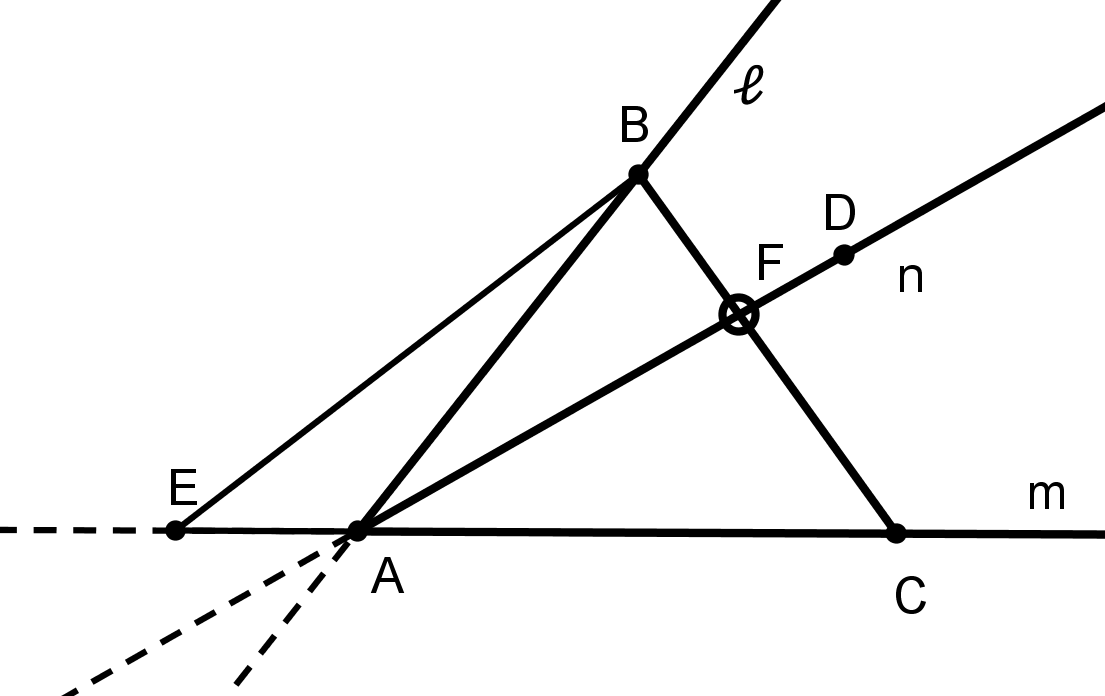
\includegraphics[width=8cm]{BILDER/1-1-09-Satz.png}}

    Die Strecke $\str{BE}$ liegt ganz auf einer Seite von $l$ und schneidet $l$ nur in $B$. Da $E$
    und $C$ auf verschiedenen Seiten von $l$ liegen, liegen alle Punkte von $\str{BE}$ auf der
    anderen Seite von $l$ wie $C$.
    \renewcommand{\labelenumi}{\arabic{enumi}.} % ändert die Nummerierung von (1) auf 1.
    \begin{enumerate}
        \item Der Strahl $\pf{AD}$ liegt im Innern des Winkels und damit ganz auf derselben Seite
            von $l$ wie $C$ (und auf derselben Seite von $m$ wie $B$) $\Rightarrow\;
            \pf{AD} \cap \str{EB} = \emptyset$.

        \item Entsprechend liegt der zu $\pf{AD}$ entgegengesetzte Strahl $\pf{AD}^* := \{X \, | \,
            \Zw(DAX)\}$ auf der anderen Seite von $m$ wie $\str{EB}$.
    \end{enumerate}
    Aus $1.$ und $2.$ folgt: $n \cap \str{EB} = \emptyset$ und daher $n \cap \str{BC} \neq
    \emptyset$, etwa $= \{F\}$.

    $F$ liegt auf $\pf{AD}$, denn $B$ und $F$ sowie $B$ und $D$ liegen auf derselben Seite von $m$,
    also auch $D$ und~$F$.
\end{proof}

\subsection{Kartesische Modelle mit Ordnung}

Ein Modell einer Ebene, die die Inzidenzaxiome erfüllt, ist die {\em kartesische Ebene} $\E_{_\K} =
\K^2$ über einem Körper $\K$.  Geraden werden, wie aus der Linearen Algebra bekannt, als Lösungen
linearer Gleichungen $a x + b y = c$ mit $a, b, c \in \R$ ($a, b$ nicht beide $0$) definiert.

Für endliche Körper erhalten wir endliche affine Geometrien, die aber nicht den Anordnungsaxiomen
genügen. Man betrachte beispielsweise "`Modell ~\ref{Modell2}"' auf Seite ~\pageref{Modell2}, dass
der kartesischen Ebene über dem Körper $\K = \{0, 1\}$ mit zwei Elementen entspricht: $\E_{\K} = \{A
= (0,0),\, B = (0,1),\, C = (1,0),\, D = (1,1)\}$.

\centerline{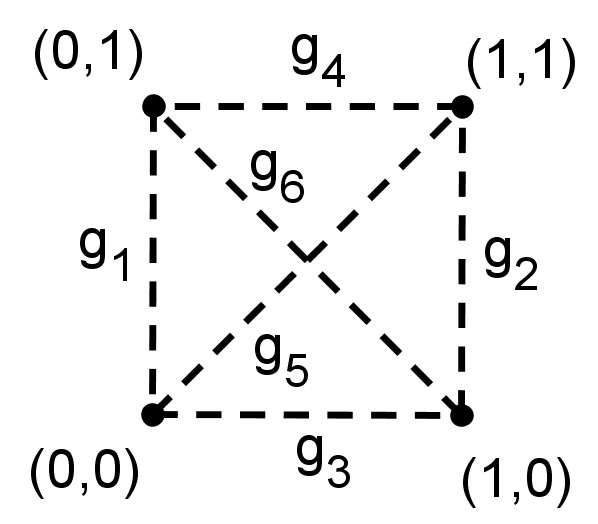
\includegraphics[width=5cm]{BILDER/1-1-10-Modell2.png}}

Es gibt allerdings eine Reihe von kartesischen Ebenen, die die Axiome der Anordnung ebenfalls
erfüllen.

\begin{defi}
    Ein Körper $K$ heißt {\em geordnet}, wenn er eine Teilmenge $K_+\subset K$ (von {\em positiven
    Elementen}) besitzt, so dass gilt:
    \renewcommand{\labelenumi}{(\roman{enumi})} % ändert die Nummerierung von (1) auf (i)
    \begin{enumerate}
        \item $\forall\, a,\, b \in K_+$ ist $a + b \in K_+$ und $a \cdot b \in K_+$;

        \item $\forall\, a \in K$ gilt genau eine der Beziehungen $a \in K_+$, $a = 0$ oder $-a \in
        K_+$.
    \end{enumerate}
\end{defi}

$\Q$ und $\R$ sind geordnet, $\C$ ist nicht geordnet.

Wenn $\K$ geordnet ist, können wir eine Ordnungsrelaton "`$<$"' definieren.
% Die Umkehrung gilt übrigens auch!! (Übung?!?)

\begin{defi}
    Sei $K$ geordnet und $a,\, b \in K$. Dann definieren wir:
    \begin{enumerate}
        \item $a > b\;: \Longleftrightarrow\; a - b \in K_+$;

        \item $a < b\;: \Longleftrightarrow\; b - a\in K_+$.
    \end{enumerate}
\end{defi}

Dies definiert eine {\em totale Ordnung} in $K$. Das heißt $\forall\, a,\, b \in K$ gilt genau eine
der Beziehungen: $a > b,\; a = b,\; a < b$.

\begin{thm}
    Sei $\K$ ein Körper und $\E_{\K}$ die entsprechende kartesische Ebene. Dann gilt:
    \begin{center}
        $\E_{\K}$ genügt den Axiomen der Anordnung $\Longleftrightarrow \K$ ist geordnet.
    \end{center}
\end{thm}

\begin{proof}
    \begin{itemize}
        \item["`$\Longrightarrow$"'] Wir betrachten die $x$-Achse $g$. Nach
            Theorem~\ref{thm:satz.s1b} wird $g$ durch $O = (0,0) \in g$ in 2 Seiten geteilt; sei

            \begin{align*}
                K_+ & := \{a \in \K:\; a \neq 0,\; (a,0) \mbox{ und } (1,0) \mbox{ liegen auf
                derselben Seite von } O\}\\
                -K_+ & := \{a \in \K:\; a \neq 0,\; (a,0) \mbox{ und } (1,0) \mbox{ liegen auf
                verschiedenen Seiten von } O\}
            \end{align*}

            Dann ist $\K = K_+ \cup \{0\} \cup -K_+$ eine disjunkte Vereinigung. Bleibt zu zeigen,
            dass mit $a, b\in K_+$ auch $a + b$ und $a \cdot b$ in $K_+$ liegen.

            \begin{description}
                \item[Addition] Die Addition $a + b$ in $\K$ entspricht dem nacheinander "`anlegen"'
                von Strecken der Längen $a$ und $b$ auf der $x$-Achse $g$ %der Addition von Strecken

                % XXX: HIER MUSS DEFINITIV NOCHMAL ÜBERDACHT WERDEN!!!!!
                % WAS SOLL UNS DAS SAGEN??? "entspricht Addition von Strecken?!?!
                % HIER BITTE EIN SAUBERES ARGUMENT!!!
                % Dieses Argument ist aus dem Buch von Hartshorne kopiert, aber nur weil die
                % "segment arithmetic" dort schon vorher behandelt wurde!!!
                % siehe Hartshorne, Proposition 15.3

                $\Rightarrow\; a + b \in K_+$

                \centerline{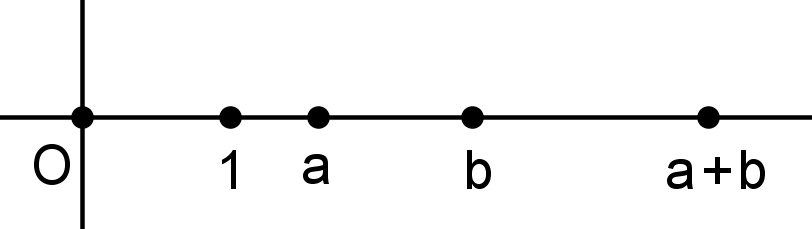
\includegraphics[width=6cm]{BILDER/1-1-16a-Satz.png}}

                \item[Multiplikation] Parallele durch $B = (0,b)$ zur Geraden durch die beiden
                    Punkte $E = (0,1),\; A = (a,0)$ schneidet $x$-Achse $g$ in $X = (a \cdot b, 0)$

                    % Beh.:  $a\cdot b\in K_+$

                    \centerline{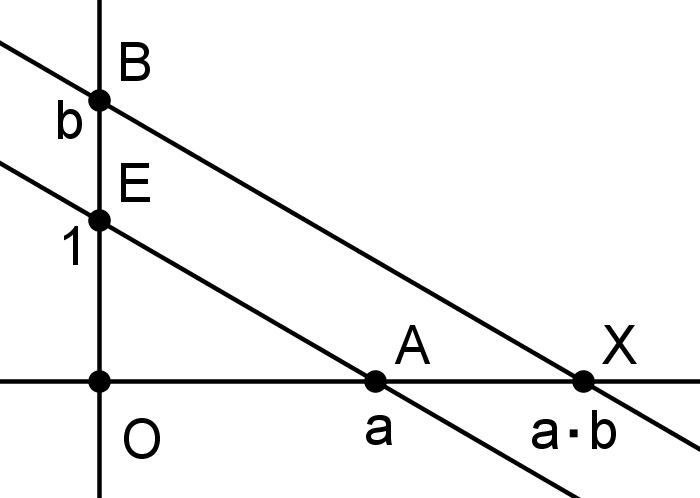
\includegraphics[width=6cm]{BILDER/1-1-16b-Satz.png}}

                    \renewcommand{\labelenumi}{\roman{enumi})} % Nummerierung: (1) -> 1)
                    \begin{enumerate}
                        \item Sei $\Zw(OEB)$ und $g(B,X)$ parallel zu $g(A,E)$. Dann liegen ganz
                            $g(B,X)$ und $O$ auf verschiedenen Seiten von $g(A,E)$, also auch
                            $\Zw(OAX)$.

                        \item Ist $\Zw(OBE)$ ergibt sich entsprechend $\Zw(OXA)$. In beiden Fällen
                            liegen daher $X$ und $A$ auf derselben Seite von $O$, also $a \cdot b
                            \in K_+$ und $K$ ist geordnet.
                    \end{enumerate}
            \end{description}

        \item["`$\Longleftarrow$"'] Sei $K$ geordnet und $A = (a_1,a_2),\; B = (b_1,b_2),\; C =
            (c_1,c_2)$ paarweise verschiedene Punkte einer Geraden $g:\; a x + b y + c = 0$.\\
            \textbf{Zwischenrelation:}

            \renewcommand{\labelenumi}{\arabic{enumi})} % ändert die Nummerierung von (1) auf 1)
            \begin{enumerate}
                \item Sei $b \neq 0: \quad \Zw(ABC)\;: \Leftrightarrow\; a_1 > b_1 > c_1$ oder
                    $a_1 < b_1 < c_1$;

                \item sei $b = 0\; (\mbox{d.h. } a_1 = b_1 = c_1 = \frac{-c}{a}):$

                    $\Zw(ABC)\;: \Leftrightarrow\; a_2 > b_2 > c_2$ oder $a_2 < b_2 < c_2$.
            \end{enumerate}

            Man prüft nun die Gültigkeit von (A1) - (A4) nach. % Übung, Blatt 3
    \end{itemize}
\end{proof}

\subsection*{Poincarésches Kreisscheibenmodell}

Ein weiteres Modell, dass den Inzidenz- und Anordnungsaxiomen genügt, ist das Poincarésche
Kreisscheibenmodell. Hierbei wählen wir die Menge der Punkte in einer offenen Kreisscheibe des
$\R^2$. (Anstelle des $\R^2$ ließe sich auch der $\K^2$ für einen anderen geordneten Köprper
verwenden.) Der Einfachheit halber wählen wir einen Kreis mit Mittelpunkt im Ursprung:

$$
    \Gamma = \{ (x,y) \in \R^2 :  x^2 + y^2 = r \}
$$

Punkte in unserem {\em  Poincaréschen Kreisscheibenmodell} sind also aus

$$
    \E = \{ (x,y) \in \R^2 :  x^2 + y^2 < r \}.
$$

Geraden sind Teile von Kreisen oder Geraden $\gamma$ des $\R^2$, die $\Gamma$ {\em orthogonal
schneiden}, d.h. die Tangenten an $\Gamma$ und $\gamma$ in den beiden Schnittpunkten liegen
orthogonal zueinander. Diese Orthogonalitätsbedingung ist im Fall einer Geraden $\gamma$ genau dann
erfüllt, wenn der Ursprung $O = (0,0)$ auf der Geraden liegt.

\centerline{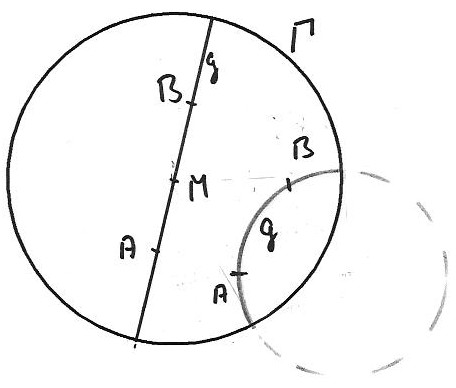
\includegraphics[width=6cm]{BILDER/4-2-04b-Geraden.jpg}}

\begin{thm} \label{thm:PoincareKreisscheibe}
    Das Poincarésche Kreisscheibenmodell genügt den Inzidenzaxiomen {\bf (I1) -- (I3)} und den
    Anordnungsaxiomen {\bf (A1) -- (A4)}.
\end{thm}

\subsection*{Inversion am Kreis}

Um zu zeigen, dass das Poincarésche Kreisscheibenmodell dem Inzidenz-Axiom {\bf (I1)} genügt,
benötigen wir zunächst ein paar Aussagen über sich orthogonal schneidende Kreise.

%% Folgendes kann man auch für beliebige Körper mit Ordnung und
%% ... machen  (Euklidische Körper!)

\begin{defi}
    $\Gamma \subset \R^2$ sei ein Kreis vom Radius $r$ und Mittelpunkt $M$. $A \in \R^2$ sei ein
    beliebiger Punkt, $A \neq M$. Sei $A' \in \pf{MA}$ derart, dass $|MA| \cdot |MA'| = r^2$
    %(solch ein Punkt $A'$ existiert stets!).
    Wir sagen, $A'$ entsteht aus $A$ durch eine \emph{Inversion} $\varphi_\Gamma :
    \R^2 \setminus\{M\} \to \R^2 \setminus \{M\}$ am Kreis $\Gamma$.
\end{defi}

\centerline{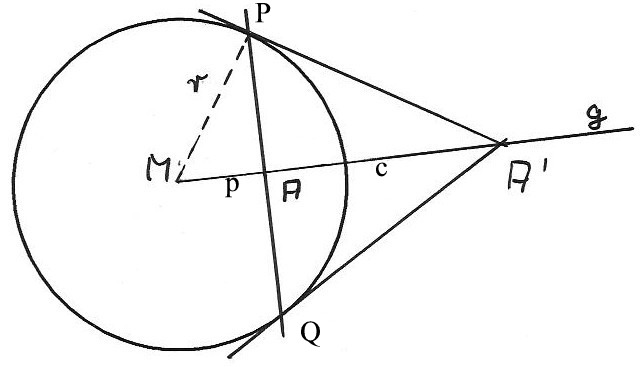
\includegraphics[width=8cm]{BILDER/4-2-01-Inversion.jpg}}

Die Punkte $A$ und $A'$ stehen in einer ganz besonderen Beziehung zueinander. Punkte außerhalb des
Kreises werden durch die Inversion am Kreis auf Punkte innerhalb des Kreises abgebildet und
umgekehrt. Liegt $A$ innerhalb des Kreises $\Gamma$, so bilden wir eine Gerade orthogonal zur
Geraden $g$ durch $M$ und $A$ durch $A$. Diese schneidet $\Gamma$ in zwei Punkten $P$ und $Q$. Die
Tangente an $\Gamma$ durch $P$ (orthogonal zu $g(M,P)$) trifft die Gerade $g$ in $A'$. Dies folgt
aus der Ähnlichkeit der Dreiecke $MPA'$ und $MAP$ und dem Verhältnis der Seitenlängen

$$
    \frac{|MA|}{r} = \frac{r}{|MA'|}.
$$

\begin{thm}\label{thm:satz.s4b}
    Inversionen $\varphi_\Gamma$ am Kreis $\Gamma$ haben folgende Eigenschaften:

    \renewcommand{\labelenumi}{\alph{enumi})} % ändert die Nummerierung von (1) auf a)
    \begin{enumerate}
        %\item[\emph{\textbf{a)}}] Kreise durch $M$ werden in Geraden $g$ mit $M\notin
        %    g$ abgebildet und umgekehrt.
        \item Ein Kreis $\gamma$, der $\Gamma$ orthogonal schneidet, wird auf sich abgebildet.

        \item Enthält ein Kreis $\gamma$ zwei einander zugeordnete Punkte $A$ und
            $A' = \varphi_\Gamma(A)$, dann schneiden sich $\gamma$ und $\Gamma$ orthogonal.

        %\item[\emph{\textbf{d)}}] Ist $\gamma$ ein Kreis und $M\notin\gamma$, dann ist
        %    $\gamma'=\varphi_\Gamma(\gamma)$ ebenfalls ein Kreis.
        %\item[\emph{\textbf{e)}}] Winkel bleiben invariant.
    \end{enumerate}
\end{thm}
%\ref{satz.s4b}

\begin{proof}
    \renewcommand{\labelenumi}{\alph{enumi})} % ändert die Nummerierung von (1) auf a)
    \begin{enumerate}
        \item Da sich $\Gamma$ und $\gamma$ orthogonal schneiden, stehen die Tangenten und Radien
            paarweise aufeinander senkrecht. Nach dem {\em Sehnen-Tangenten-Satz}
            %(Übung, Blatt 3!!)
            gilt
            $$
                |MA| \cdot |MA'| = |MP|^2 = r^2.
            $$
            \centerline{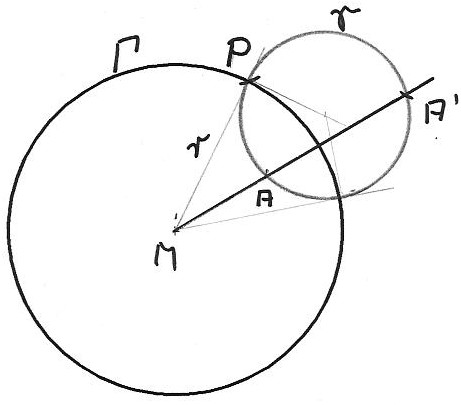
\includegraphics[width=6cm]{BILDER/4-2-02b-Inversion.jpg}}

        \item Gibt es umgekehrt $A,\, A' \in \gamma$ mit $|MA| \cdot |MA'| = r^2$, dann müssen sich
            $\Gamma$ und $\gamma$ schneiden. Sei $P$ ein Schnittpunkt von $\Gamma$ und $\gamma$.
            Dann ist $|MP| = r$, also $|MP|^2 = |MA| \cdot |MA'|$ und $|MP|$ ist Tangentenabschnitt
            für $\gamma$, auf dem der Radius von $\gamma$ orthogonal steht.
    \end{enumerate}
\end{proof}

Das Theorem zeigt insbesondere, dass das gesamte {\em Kreisbüschel} (Menge von Kreisen) durch zwei
Punkte $A$ und $\varphi_\Gamma(A)$ den Kreis $\Gamma$ orthogonal schneidet. Liegt $A$ im Inneren
der Kreisscheibe, so entsprechen die Schnitte des Kreisbüschels mit dem Inneren der Kreisscheibe,
allen Geraden durch $A$ im Poincaréschen Kreisscheibenmodel.

\centerline{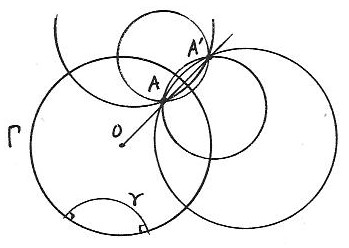
\includegraphics[width=6cm]{BILDER/4-2-06-Parallel.jpg}}

Betrachtet man eine Gerade $g$ (bzw. einen orthogonal schneidenden Kreis $\gamma$) außerhalb von
$A$, so sieht man auch, dass das Parallelenaxiom in der Poincaréschen Kreisscheibe nicht gilt.

\subsection*{Inzidenz und Anordnung im Kreisscheibenmodell}

Die Axiome der Inzidenz und Anordnung gelten allerdings in der Poincaréschen Kreisscheibe. Dazu
erklären wir die Beziehung "`Zwischen"' wie folgt: seien $A,\, B,\, C \in \E$ kollinear. Liegen
$A,\, B,\, C$ auf einem Durchmesser, also einer Geraden des $\R^2$, dann sei $Zw(ABC)$ wie im $\R^2$
erklärt. Liegen $A,\, B,\, C$ auf einem Kreis $\gamma$ mit Mittelpunkt $M'$, dann ziehen wir von
$M'$ die Strahlen zu $A,\, B,\, C$, diese treffen die Verbindungsstrecke der beiden Schnittpunkte
von $\gamma$ und $\Gamma$ in $A',\, B',\, C'$. Wir definieren $Zw(ABC)\; \Leftrightarrow\;
Zw(A'B'C')$ im Sinne des $\R^2$.

\centerline{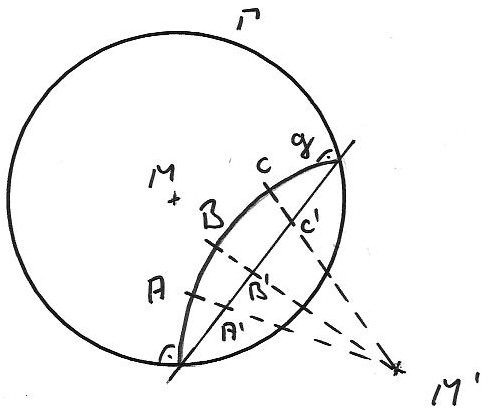
\includegraphics[width=6cm]{BILDER/4-2-07-Zwischen.jpg}}

\begin{proof}[Beweis von Theorem~\ref{thm:PoincareKreisscheibe}]
    {\bf (I2), (I3)} sind sicher erfüllt, genau so wie {\bf (A1) - (A3)}. %(Übung)??
    \begin{description}
        \item[(I1)] Seien $A,\, B \in \E$
            \begin{enumerate}
                \item $M,\, A,\, B$ kollinear $\Rightarrow\; \E$-Gerade ist der Durchmesser durch
                    $A$ und $B$.

                \item $M,\, A,\, B$ nicht kollinear, $A' = \varphi_\Gamma(A)\; \Rightarrow\;
                    \exists$ genau einen Kreis $\gamma$ durch $A,\, B,\, A'$, $\gamma$ ist
                    orthogonal zu $\Gamma$ nach Theorem~\ref{thm:satz.s4b}, b); ebenfalls $B' \in
                    \gamma$ nach Theorem~\ref{thm:satz.s4b} (a).
            \end{enumerate}
    \end{description}
\end{proof}

\begin{description}
    \item[(A4) -- Axiom von Pasch] Gegeben sei das Dreieck $ABC\subset\E$. Je 2 Geraden (Kreise)
        schneiden sich innerhalb $\Gamma$ in genau 1 Punkt $X$ (der 2. Schnittpunkt $X' =
        \varphi_\Gamma(X)$ liegt außerhalb von $\Gamma$ (Übungsaufgabe).
\end{description}

$\Rightarrow$ Inneres des Dreiecks $ABC$ ist wohldefiniert (2 Punkte auf derselben Seite der
$\E$-Geraden $\Longleftrightarrow$ beide Punkte innerhalb oder außerhalb des Kreises)

\centerline{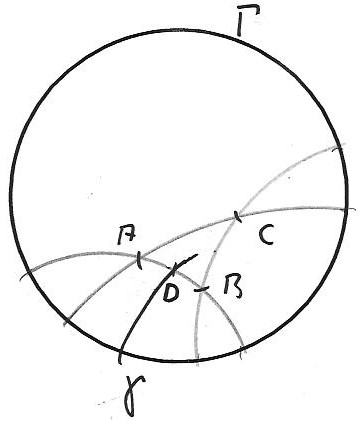
\includegraphics[width=5cm]{BILDER/4-2-08-Pasch.jpg}}

Ist $g$ eine $\E$-Gerade mit Kreis $\gamma$, die durch keinen der Eckpunkte $A,\, B,\, C$ geht und
etwa $\str{AB}$ in $D$ schneidet, dann liegen $A$ und $B$ auf verschiedenen Seiten von $g$, etwa $B$
innerhalb $\gamma$. Angenommen, $B,\, C$ auf derselben Seite von $\gamma$, etwa beide innerhalb
$\gamma\; \Rightarrow$ der Kreis durch $A,\, C$ enthält $A$ außerhalb und $C$ innerhalb von
$\gamma\; \Rightarrow\; \exists$ Schnittpunkt auf $AC$.

\section*{Vorlesung am 03.05.2011}
% Vertretung durch Thomas

\subsection*{Axiome der Kongruenz, Strecken}

Wir führen eine Relation zwischen Strecken (und später auch zwischen Winkeln) ein und nennen diese
"`Kongruenz"', in Zeichen $\str{AB} \cong \str{CD}$, wenn folgende Axiome erfüllt sind: 
%(Kongruenz ist in einem erweiterten Sinn eine "`{}Gleichheit"'{}):

\begin{enumerate}
    \item[{\bf (C1)}] (Existenz) Sei $\str{AB} \subset \E\; (A \neq B)$ und $C$ der Ursprung eines
        Strahls $r$. Dann gibt es genau einen Punkt $D \in r,\; D \neq C,$ mit $\str{AB} \cong
        \str{CD}$.

    %\includegraphics[width=3.5cm]{1-2-01-C1}

    \item[{\bf (C2)}] Wenn 2 Strecken einer dritten kongruent sind, dann sind sie zueinander kongruent:

        $$
            \str{AB} \cong \str{CD} \mbox{ und } \str{AB} \cong \str{EF}\; \Rightarrow\; \str{CD} \cong \str{EF}.
        $$

        Jede Strecke ist zu sich selbst kongruent.

    \item[{\bf (C3)}] (Addition) Wenn $A,\,B,\,C\in \E$ und $Zw(ABC)$\\
        sowie $D,\, E,\, F \in \E$ mit $Zw(DEF)$ und\\
        $\str{AB} \cong \str{DE}$, $\str{BC} \cong \str{EF}$, dann ist auch $\str{AC} \cong
        \str{DF}$.

    %\includegraphics[width=4cm]{1-2-01-C3}
\end{enumerate}

\begin{thm}\label{thm:satz.s1d}
    Die Kongruenz von Strecken ist eine Äquivalenzrelation.
\end{thm}
%\ref{satz.s1d}

\begin{proof}
    Übungsaufgabe.
\end{proof}

Die Definition der Kongruenz von Strecken erlaubt uns auch mit Strecken zu rechnen.

\begin{defi}[Addition von Strecken]\label{def:d1a}
    Seien $\str{AB}$ und $\str{CD}$ Strecken, $r = \pf{AB}$ ein Strahl. Ist $E$ der eindeutig
    bestimmte Punkt auf $r$, so dass $\str{BE} \cong \str{CD}$ nach \textbf{(C1)}, dann heißt
    $\str{AE}$ {\em die Summe von $\str{AB}$ und $\str{CD}$}:

    $$
        \str{AB} + \str{CD} := \str{AE}.
    $$
\end{defi}

\centerline{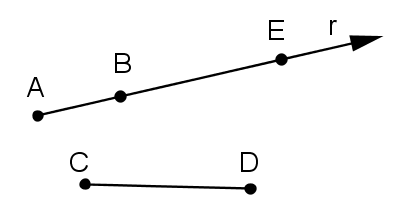
\includegraphics[width=5cm]{BILDER/1-2-02-Add.png}}

Die Addition ist eine wohldefinierte Operation auf den Äquivalenzklassen kongruenter Strecken, wie
die folgende Aussage belegt.

%% BEMERKUNG: Man kann auch zeigen, dass die Addition assoziativ und
%% als Operation auf den Äquivalenzklassen kommutativ ist.
%% Siehe Hartshorne, Excercise 8.1

\begin{thm}\label{thm:satz.s1e}
    Sei $\str{AB} \cong \str{A'B'}$ und $\str{CD} \cong \str{C'D'}\; \Longrightarrow\; \str{AB} +
    \str{CD} \cong \str{A'B'} + \str{C'D'}$

    Das heißt die Addition von Strecken ist unabhängig von den ausgewählten Repräsentanten.
\end{thm}
%\ref{satz.s1e}

\begin{proof}
    Sei $E$ wie in Definition~\ref{def:d1a}: $\str{AE} = \str{AB}+\str{CD}$ und entsprechend $E':$

    $$
        \str{A'E'} = \str{A'B'} + \str{C'D'}
    $$

    Daraus folgt $\str{BE} \cong \str{CD} \cong \str{C'D'} \cong \str{B'E'} \Longrightarrow\;
    \str{BE} \cong \str{B'E'}$ nach (\ref{thm:satz.s1d}) $\Longrightarrow$ (C3)
    $\str{AE}\cong\str{A'E'}$.

    \centerline{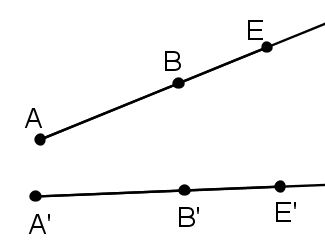
\includegraphics[width=5cm]{BILDER/1-2-03-Add.png}}
\end{proof}

\begin{thm}[Differenz von Strecken]\label{thm:satz.s1f}
    Seien $A,\, B,\, C$ kollinear mit $Zw(ABC)$ und $E,F$ seien zwei Punkte auf einem Strahl
    $\pf{DE}$ mit {\em Ausgangspunkt} $D$, so dass $\str{AB} \cong \str{DE}$ und $\str{AC} \cong
    \str{DF}$. Dann gilt $Zw(DEF)$ und $\str{BC} \cong \str{EF}$.  ($\str{BC}$ heißt
    \emph{Differenz} von $\str{AC}$ und $\str{AB}$.)
\end{thm}

\begin{proof}
    Sei $F'$ auf dem Strahl $\pf{DE}$ gewählt, so dass $Zw(DEF')$ und $\str{BC} \cong \str{EF'}$
    nach (C1) $\stackrel{(C3)}{\Longrightarrow}$ $\str{AC} \cong \str{DF'}$. Die Punkte $F$ und
    $F'$ liegen beide auf $\pf{DE}$. Ausserdem gilt $\str{AC} \cong \str{DF}$, so dass aus (C2) und
    der Eindeutigkeit in (C1), auch $F=F'$ folgt. Also auch $Zw(DEF)$.

    \centerline{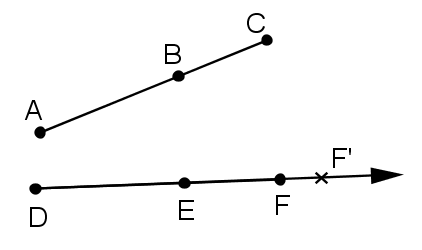
\includegraphics[width=5cm]{BILDER/1-2-04-Diff.png}}
\end{proof}

Es ist auch möglich Strecken miteinander zu vergleichen:

\begin{defi}
    Seien $\str{AB}$ und $\str{CD}$ Strecken in $\E$. Dann sei $\str{AB} < \str{CD}\;:
    \Leftrightarrow\; \exists\, E \in \str{CD},\; Zw(CED)$ und $\str{AB} \cong \str{CE}$.
\end{defi}

\centerline{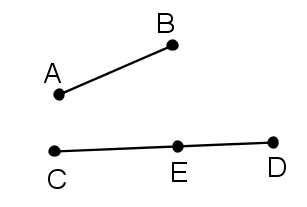
\includegraphics[width=5cm]{BILDER/1-2-05-Ord.png}}

\begin{thm}\label{thm:satz.s1g}\ % Das erzwungene Leerzeichen sorgt für den Umbruch.
    \renewcommand{\labelenumi}{\alph{enumi})} % ändert die Nummerierung von (1) auf a)
    \renewcommand{\labelenumii}{\alph{enumi}\textsubscript{\arabic{enumii}})}
        % Nummerierung 2. Ebene
    \begin{enumerate}
        \item\label{thm:satz.slg.item1} Ist $\str{AB} \cong \str{A'B'}$ und $\str{CD} \cong
            \str{C'D'}\; \Longrightarrow\; \{\str{AB} < \str{CD} \Leftrightarrow \str{A'B'} <
            \str{C'D'}\}$

        \item "`$ < $"' ist eine Ordnungsrelation in der Menge aller Strecken, d.h.
            \begin{enumerate}
                \item\label{thm:satz.slg.item2-1} $\str{AB} < \str{CD}$ und $\str{CD} < \str{EF}\;
                    \Longrightarrow \; \str{AB} < \str{EF}$

                \item\label{thm:satz.slg.item2-2} $\forall$ Strecken $\str{AB},\, \str{CD} \subset
                    \E$ gilt genau eine der Relationen

                    $\str{AB} < \str{CD},\; \str{AB} = \str{CD}$ oder $\str{AB}>\str{CD}$.
            \end{enumerate}
    \end{enumerate}
\end{thm}

\begin{proof}
    \begin{enumerate}
        \item[zu ~\ref{thm:satz.slg.item1}.]\ % erzwungenes Leerzeichen => Umbruch
            \begin{itemize}
                \item["`$\Longrightarrow$"'] Sei $\str{AB} < \str{CD} \Longrightarrow\; \exists\, E
                    \in \str{CD},\; Zw(CED)$ und $\str{AB} \cong \str{CE}\;
                    \stackrel{(C1)}{\Longrightarrow}\; \exists\, E' \in r':\; \str{CE} \cong
                    \str{C'E'}$ und $D',\, E'$ auf derselben Seite von $C'$.  Wegen $\str{CD} \cong
                    \str{C'D'}$ und Theorem~\ref{thm:satz.s1f} folgt $Zw(C'E'D')$ und $\str{A'B'}
                    \cong \str{CE} \cong \str{C'E'}$, also $\str{A'B'} < \str{C'D'}$.

                \item["`$\Longleftarrow$"'] genauso.

                \centerline{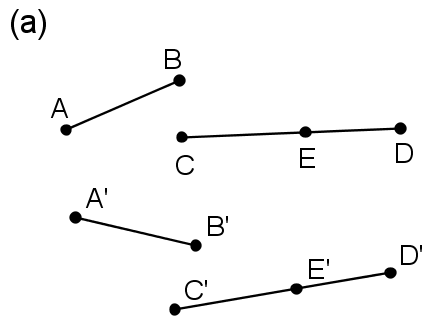
\includegraphics[width=5cm]{BILDER/1-2-06a-Ord.png}}
            \end{itemize}

            % \textbf{b)} Dem Beweis von b) stellen wir folgende Aussage voran:

            % \begin{lemma}\label{lemma.l1d}
            % Sind $A,B,C\in g$ kollinear und $Zw(ABC)$, dann liegen $A,\,B$ auf
            % derselben Seite von $C$ und $B,\,C$ auf derselben Seite von $A$
            % \emph{(sonst $Zw(ACB)$ bzw. $Zw(BAC)$)}. Gilt dann auch noch
            % $Zw(ACD)$, also $A$ und $D$ auf verschiedenen Seiten von $C$, dann
            % liegen $A$ und $D$ auch auf verschiedenen Seiten von $B$ und $B$
            % und $D$ auf verschiedenen Seiten von $C$, also $Zw(ABD)$ und
            % $Zw(BCD)$.
            % \end{lemma}
            % %\ref{lemma.l1d}
            % Wir haben das Bild: \qquad\qquad
            % \includegraphics[width=6cm]{1-2-07-Ord}

            % \textbf{Beweis zu \ref{lemma.l1d}} Mit den Bezeichnungen aus
            % Abschnitt 1.1 gilt:
            % \[Zw(ABC)\wedge Zw(ACD)\;\Longrightarrow\;A\stackrel{C}{\sim}
            % B\;\mbox{und}\;A\stackrel{C}{\nsim}D\;\Longrightarrow\;
            % B\stackrel{C}{\nsim}D\;\Longrightarrow\; Zw(BCD)\] und
            % \[Zw(BCD)\wedge Zw(ABC)\;\Longrightarrow\;C\stackrel{B}{\sim}
            % D\;\mbox{und}\;A\stackrel{B}{\nsim}C\;\Longrightarrow\;
            % A\stackrel{B}{\nsim}D\;\Longrightarrow\; Zw(ABD),\] qed.

        \item[zu ~\ref{thm:satz.slg.item2-1}.] Sei $\str{AB} \cong \str{CX}$ mit $Zw(CXD)$ sowie
            $\str{CD} \cong \str{EY}$ mit $Zw(EYF)$. Nach Theorem~\ref{thm:satz.s1f} gibt es ein $Z
            \in \str{EY}$ mit $\str{CX} \cong \str{EZ}$. Aus $Zw(EYF)$ und $Zw(EZY)$ folgt
            % aus Lemma \ref{lemma.l1d} 
            $Zw(EZF)$ (Übung). % ACHTUNG: Diese Aussage ist nicht trivial!
            Also $\str{AB} < \str{EF}$.

            \centerline{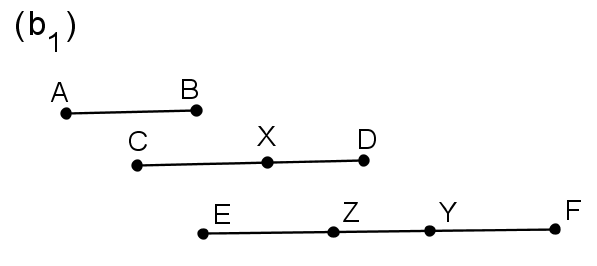
\includegraphics[width=5cm]{BILDER/1-2-06b1-Ord.png}}

        \item[zu ~\ref{thm:satz.slg.item2-2}.] Sei $r = \overrightarrow{CD}$ und $E \in r$ derart,
            dass $\str{AB} \cong \str{CE}\; \Longrightarrow\; Zw(CED)\; (\str{AB} < \str{CD})$ oder
            $E = D\; (\str{AB} \cong \str{CD})$ oder $Zw(CDE)\; (\str{AB} > \str{CD})$.

            \centerline{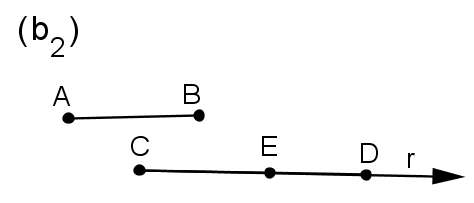
\includegraphics[width=5cm]{BILDER/1-2-06b2-Ord.png}}
    \end{enumerate}
\end{proof}

\subsection*{Kongruenz von Strecken für geordnete Körper}

Die Kongruenz von Strecken in der kartesischen Ebene $\K^2$ kann wie gewohnt über die {\em
Distanzfunktion} erklärt werden. Für zwei Punkte $A = (a_1,a_2)$ und $B = (b_1,b_2)$ ist die Distanz
erklärt durch

$$
    \dist(A,B) := \sqrt{(a_1-b_1)^2 + (a_2-b_2)^2} .
$$

Wenn die Wurzel und damit die Distanzfunktion im Körper $\K$ erklärt ist, erklären wir zwei Strecken
$AB$ und $CD$ {\em kongruent}, wenn $\dist(A,B) = \dist(C,D)$. Das ist natürlich genau dann der
Fall, wenn

$$
\dist^2(A,B) = (a_1 - b_1)^2 + (a_2 - b_2)^2 = (c_1 - d_1)^2 + (c_2 - d_2)^2 = \dist^2(C,D).
$$

Letztere Bedingung hat den Vorteil, dass sie auch in Körpern $\K$ definiert ist, in denen nicht alle
Wurzeln existieren.

%Wenn die Wurzel in $\K$ nicht erklärt ist, können wir Strecken $AB$ und $CD$ deshalb
%einfach kongruent erklären wenn die entsprechende Gleichheit für die
%Quadrate der Distanzfunktion gilt, d.h., wenn $\dist^2(A,B) =
%\dist^2(C,D)$.

Man könnte die Kongruenz auch über andere Distanzfunktionen erklären, etwa über

$$
    \dist_1(A,B) := |a_1 - b_1| + |a_2 - b_2|
$$

oder

$$
    \dist_{\infty}(A,B) := \sup \{ |a_1 - b_1|, |a_2 - b_2| \}.
$$

% ACHTUNG: Dabei bekäme man aber Geometrien heraus, die nicht isomorph
% zur oben erklärten sind!! (untereinander wären die beiden aber
% durchaus isomorph!)
% siehe Hartshorne, Übungen 8.7-8.9

Für einen geordneten Körper $\K$ gilt $\dist^2(A,B) > 0$ genau dann wenn $A, B\in \K^2$ verschieden
sind.

\begin{thm}
    In der kartesischen Ebene $\E_{\K} = \K^2$ über einem geordneten Körper $\K$ gelten die
    Kongruenzaxiome {\bf (C2)} und  {\bf (C3)}. Das Kongruenzaxiom {\bf (C1)} gilt genau dann, wenn
    es zu jedem Element $a \in \K$ auch die Wurzel von $1 + a^2$ in $\K$ gibt. ($\K$ heißt in diesem
    Fall {\em Pythagoreischer Körper}).
\end{thm}

Man beachte, dass wir im Kapitel über Euklids Elemente gesehen haben, dass die Konstruktionen mit
Zirkel und Lineal immer innerhalb eines {\em Pythagoreischen Körpers} stattfinden.

% d.h., wenn wir die Punkte mit denen wir beginnen aus $\K^2$ wählen, bleiben wir auch in $\K^2$...

\begin{proof}
    Das Kongruenzaxiom {\bf (C2)} ist eine einfache Folgerung aus der Definition von $\dist^2(A,B)$.
    Der Nachweis von {\bf (C3)} bleibt als Übungsaufgabe.

    %{\bf TO BE FILLED:  Parts of proof of Proposition 16.1 in Hartshorne!}

    Für die Äquivalenzaussage über {\bf (C1)} zeigen wir zunächst, dass die Aussage nicht für
    beliebige Körper gilt. Für $a\in \K$ betrachten wir dazu die Strecke $OA$ mit $O = (0,0)$ und $A
    = (a,1)$. Um zur Strecke $OA$ eine kongruente Strecke $OB$ auf der x-Achse "`abzutragen"',
    benötigen wir einen Punkt $B = (b,0)$ mit $\dist^2(O,A) = \dist^2(O,B)$, also mit

    $$
        1 + a^2 = b^2.
    $$

    Mit anderen Worten: Wir benötigen ein Element $b \in \K$, dass die Wurzel von $1 + a^2$ ist.

    Umgekehrt: Angenommen für jedes $c\in \K$ gibt es ein Element $\sqrt{1 + c^2} \in \K$. Dann
    können wir für jedes Paar $a, b \in \K$, mit $a \not = 0$, die Wurzel aus $a^2 + b^2$ in $\K$
    finden: Zunächst gilt

    $$
        a^2+b^2 = a^2 \left(1+ \left(\frac{b}{a}\right)^2 \right).
    $$

    Mit $c = b/a$ gilt dann

    $$
        \sqrt{a^2 + b^2} = |a| \cdot \sqrt{1 + c^2}.
    $$

    %% ACHTUNG: Ist der Betrag überhaupt in $K$ erklärt!!?? (Ja weil, $K$ geordnet).
    Man beachte: Der Betrag $|a|$ von $a$ erklärt ist weil $\K$ geordnet ist; und wir haben durch
    obiges Argument gezeigt, dass in {\em Pythagoreischen Körpern} $\K$ die Distanz $\dist(A,B)$ von
    Strecken in $\E_{\K}$ immer auch ein Element des Körpers ist.

    Sei $g$ eine Gerade in $\E_{\K}$ beschrieben durch $y = m x + b$, mit $m, b \in \K$. Für einen
    beliebigen Punkt $A = (a, m a + b)$ auf $g$ und ein $d \in \K$ wollen wir eine Strecke $AC$ der
    Länge $d$ auf $g$ abtragen. D.h., für $C = (c, m c + b)$ gilt

    $$
        \dist(AC) = \sqrt{(a - c)^2 + ( (m a + b) - (m c + b) )^2} = d,
    $$

    bzw.

    $$
        |a-c| \cdot \sqrt{1 + m^2} = d.
    $$

    Da $\sqrt{1 + m^2} \in \K$ nach Voraussetzung, lässt sich die letzte Gleichung in $\K$ nach $c$
    auflösen. Dabei erhalten wir zwei Lösungen für die beiden möglichen Richtungen, in denen die
    Strecke $AC$ abgetragen werden kann.
\end{proof}

\begin{bem}
    An dieser Stelle könnte man noch als zweites Beispiel die Kongruenz von Strecken in der
    Poincaréschen Kreisscheibe erklären. Dazu müsste man nur das Doppelverhältnis von vier Punkten
    in der Kartesischen Ebene definieren (siehe Hartshorne, S.339) und dann die ``$P$-Kongruenz'' am
    Kreis erklären (siehe Hartshorne, S.358). Ein Beweis, dass (C1) -- (C3) erfüllt sind, sollte an
    dieser Stelle nicht gegeben werden.
\end{bem}

\section*{Vorlesung am 05.05.2011}
% Vertretung durch Thomas

\subsection*{Kongruenz von Winkeln}

\begin{enumerate}
    \item[{\bf(C4)}] (Existenz) Gegeben sei der Winkel $\wi(BAC)$ und ein Strahl $\pf{DE}$. Dann
        existiert ein eindeutig bestimmter Strahl $\pf{DF}$ auf einer vorgegebenen Seite von
        $g(D,E)$, so dass $\wi(BAC) \cong \wi(EDF)$.

        \centerline{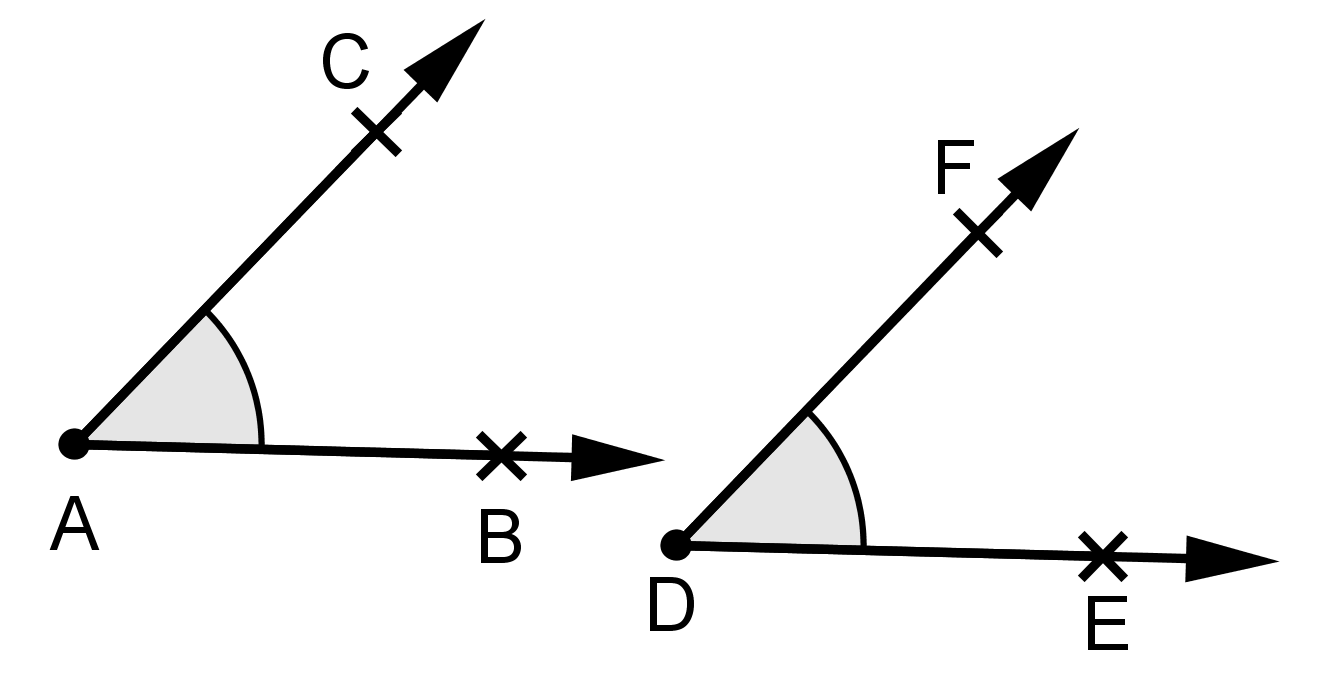
\includegraphics[width=5cm]{BILDER/1-2-08-C4.png}}

    \item[{\bf(C5)}] Für je 3 Winkel $\alpha,\, \beta,\, \gamma$ gilt: $\alpha \cong \beta$ und
        $\alpha \cong \gamma\; \Longrightarrow\; \beta \cong \gamma$\\

        %% KOMMENTAR NESSELMAN: (Woher?? Warum??)
        %    (Diese Aussage ist aus dem Rest beweisbar, so ist es aber bequemer!)\\
        %
        % FOLGENDE Reflexivität war im Nesselmann-Skript Teil von C4!?!?
        % Wir folgen hier Hartshorne...

        Jeder Winkel ist zu sich selbst kongruent: $\wi(BAC) \cong \wi(BAC)$.

    \item[{\bf(C6)}] Gilt für 2 Dreiecke $ABC$ und $DEF$: $\str{AB} \cong \str{DE},\; \str{AC} \cong
        \str{DF}$ und $\wi(BAC) \cong \wi(EDF)\; \Longrightarrow\; \wi(ABC) \cong \wi(DEF)$

        % (und damit durch Bezeichnungswechsel auch
        % $\wi(BCA)\cong\wi(EFD)\;\Longrightarrow$
        % die Dreiecke sind "`{}kongruent"'{})
        % Beweis siehe Hilbert \cite{Hil}, I.5)

    \centerline{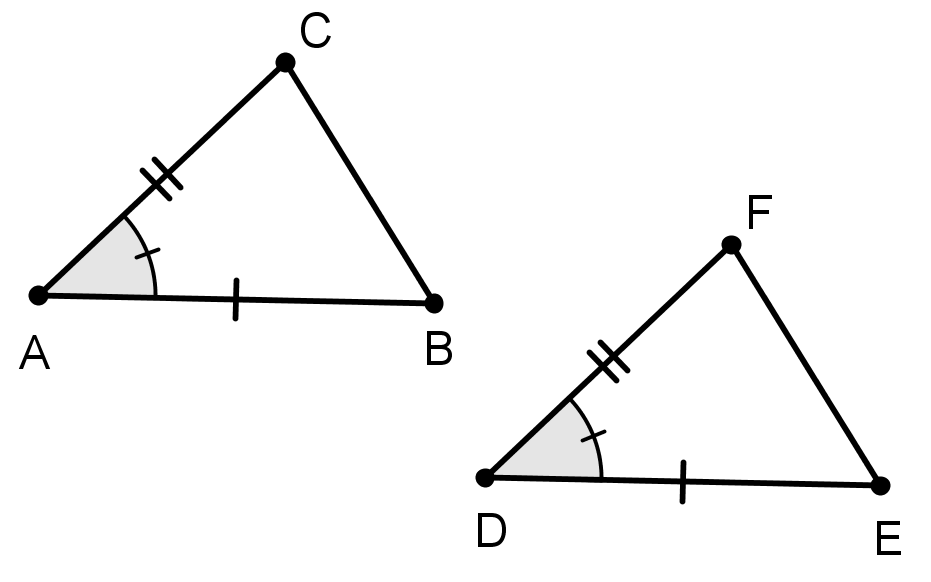
\includegraphics[width=5cm]{BILDER/1-2-08-C6.png}}
\end{enumerate}

\begin{bem}
    \renewcommand{\labelenumi}{\alph{enumi})} % ändert die Nummerierung von (1) auf a)
    \begin{enumerate}
        \item Nach den Kongruenzaxiomen wird weder der Strecke noch dem Winkel eine Richtung
            (Orientierung) zugeordnet.

        \item Axiom (C6) gewährleistet die Homogenität der Ebene, d.h. die Ebene verhält sich an
            jedem Punkt gleich.

        \item Die Kongruenzrelation der Winkel ist eine äquivalenzrelation (direkte Folge aus (C5)).
    \end{enumerate}
\end{bem}

\begin{defi}[Hilbert-Ebene]
    Eine Ebene, in der die Axiome {\bf (I1) -- (I3)}, {\bf (A1) -- (A4)} und {\bf (C1) --(C6)}
    gelten, heißt {\em Hilbert-Ebene}.
\end{defi}

\begin{bem}
    An dieser Stelle sollte man erklären, dass sich die Kongruenz von Winkeln in Kartesischen Ebenen
    $\E_{\K}$ über den Tangenz erklären lässt (siehe Hartshorne, S.141ff). Der Nachweis, dass (C6)
    gültig ist, ist dann etwas aufwendiger. Die Kongruenz von Winkeln in der Poincaréschen
    Kreisscheibe ist wie in der Kartesischen Ebene erklärt. An dieser Stelle sollte man es deshalb
    wohl dabei belassen zu erwähnen, dass es diese beiden Besipiele gibt (ohne es zu beweisen).
\end{bem}

%% Vgl. dazu Stillwell, Section 3.5!

\subsection*{Kongruenz von Dreiecken}

Ein wesentlicher Teil der aus der euklidischen Geometrie bekannten Dreiecksgeometrie lässt sich
bereits in einer Hilbert-Ebene beweisen.

% und ist damit Bestandteil der absoluten Geometrie.
% WAS SOLL DAS DENN HEISSEN?? Niemand weiß was "absolute Geometrie"
% ist an dieser Stelle...

% ACHTUNG: Die kurze Notation  $\wi{A}$, etc... wird ab hier immer
% wieder verwendet! Sollte vielleicht drauf hingewiesen werden...

\begin{defi}[Kongruenz von Dreiecken]
    Zwei Dreiecke $ABC$ und $DEF$ heißen {\em kongruent} $:\Longleftrightarrow$\\
    $\str{AB} \cong \str{DE},\; \str{AC} \cong \str{DF},\; \str{BC} \cong \str{EF}$ und $\wi{A}
    \cong \wi{D},\; \wi{B} \cong \wi{E},\; \wi{C} \cong \wi{F}$, d.h. Seiten und Winkel sind
    paarweise zueinander kongruent: $ABC \cong DEF$
\end{defi}

\centerline{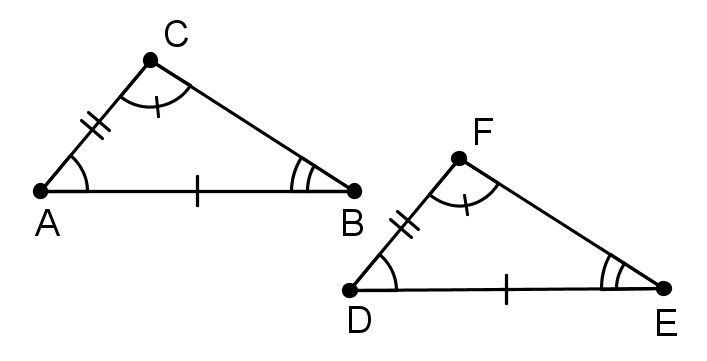
\includegraphics[width=5cm]{BILDER/1-2-09-Kongruenz.png}}

\begin{thm}[SWS-Kriterium]\label{thm:satz.s1h}
    Dreiecke, die den Bedingungen von {\bf (C6)} genügen, sind kongruent.
\end{thm}
%\ref{satz.s1h}

\begin{proof}
    Nach (C6) ist $\wi B \cong \wi E$ und $\wi C \cong \wi F$. Wir müssen noch $\str{BC} \cong
    \str{EF}$ zeigen.

    Sei $F'$ derart, dass $\str{BC} \cong \str{EF'}$ und etwa $F'\neq F$
    $\stackrel{(C6)}{\Longrightarrow} \wi(BAC) \cong \wi(EDF')$ und nach Voraussetzung $\wi(BAC)
    \cong \wi(EDF)$ im Widerspruch zu (C4) $\Longrightarrow\; F' = F$.
\end{proof}

\centerline{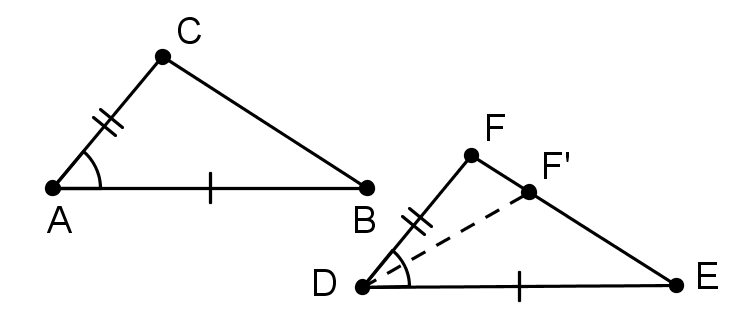
\includegraphics[width=5cm]{BILDER/1-2-10-SWS.png}}

Genauso erhält man:

\begin{thm}[WSW-Kriterium]\label{thm:satz.s1i}
    Gelten für 2 Dreiecke $ABC$ und $DEF$ die Kongruenzen $\str{AC} \cong \str{DF},\;\wi A \cong \wi
    D,\; \wi B \cong \wi E\; \Longrightarrow\; ABC \cong DEF$, d.h. die Dreiecke sind kongruent.
\end{thm}
%\ref{satz.s1i}

\begin{proof}
    Wie oben tragen wir $\str{BC}$ auf dem Strahl $\pf{EF}$ ab $\Longrightarrow\; \exists\, F':\;
    \str{BC} \cong \str{EF'}\; \stackrel{(C6)}{\Longrightarrow} \; ABC \cong DEF'$ und $\wi(EDF')
    \cong \wi(BAC) \cong \wi(EDF)$.

    Falls $F' \neq F\; \Longrightarrow\; \wi(EDF') < \wi(EDF)$ oder $\wi(EDF') > \wi(EDF)$ -
    Widerspruch.
\end{proof}

\centerline{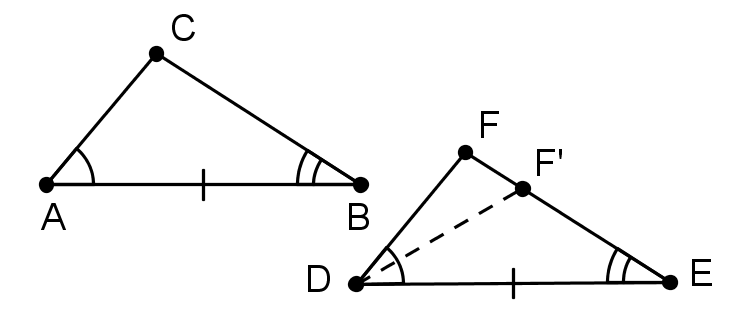
\includegraphics[width=5cm]{BILDER/1-2-11-WSW.png}}

\begin{thm}[SSS-Kriterium]\label{thm:satz.s1n}
    Wenn in zwei Dreiecken $ABC$ und $A'B'C'$ gilt $\str{AB} \cong \str{A'B'},\; \str{AC} \cong
    \str{A'C'}$ und $\str{BC} \cong \str{B'C'}$, dann ist $ABC \cong A'B'C'$.
\end{thm}
%\ref{satz.s1n}

Für den Beweis des SSS-Kriteriums benötigt man erheblich mehr Aufwand. Wir kommen darauf zurück\dots

\subsection*{Rechnen mit Winkeln}

Wie bei den Kongruenzaxiomen für Strecken, lassen sich auch für Winkel Summe, Differenz und eine
Ordnungsrelation erklären.

\begin{defi}\
    \renewcommand{\labelenumi}{\alph{enumi})} % ändert die Nummerierung von (1) auf a)
    \begin{description}
        \item[Summe von 2 Winkeln] Sei $\wi(BAC)$ ein Winkel und \pf{AD} ein Strahl im Innern, dann
            heißt $\wi(BAC)$ die Summe von $\wi(BAD)$ und $\wi(DAC)$.

            \centerline{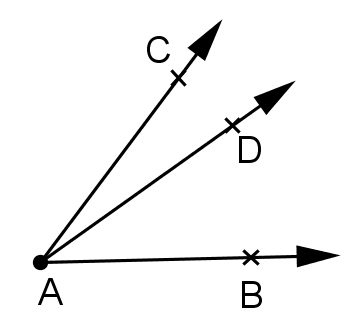
\includegraphics[width=5cm]{BILDER/1-2-12a-Winkel.png}}

        \item[Nebenwinkel] Sei $\wi(BAC)$ ein Winkel und $D \in g(A,C)$ auf der anderen Seite von
            $A$ wie $C$. Die Winkel $\wi(BAC)$ und $\wi(BAD)$ heißen \emph{Nebenwinkel}.

            %% ACHTUNG:
            % Hier sollte ein Bild zur Definition des Nebenwinkels hin, mit
            % C,A,D auf einer Geraden ; entsprechend sollte das Bild (die
            % Bezeichnungen) zur Definition des Rechten Winkels angepasst werden!

        \item[Scheitelwinkel] $\wi(BAC)$ und $\wi(DAE)$ heißen \emph{Scheitelwinkel}.

            \centerline{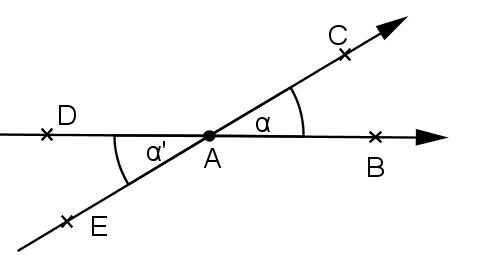
\includegraphics[width=5cm]{BILDER/1-2-12c-Winkel.png}}

        \item[rechter Winkel -- Rechter] $\alpha$ heißt ein \emph{rechter Winkel} oder
            \emph{Rechter} $:\Longleftrightarrow\; \alpha$ ist zu seinem Nebenwinkel kongruent
            ($\alpha\cong\beta$).

        \centerline{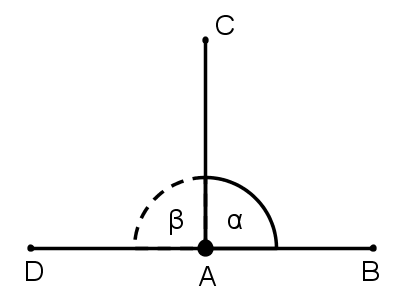
\includegraphics[width=5cm]{BILDER/1-2-12d-Rechter.png}}
    \end{description}
\end{defi}

\begin{thm}\label{thm:satz.s1k}
    Sind $\wi(BAC)$ und $\wi(BAD)$ sowie $\wi(B'A'C')$ und $\wi(B'A'D')$ paarweise Nebenwinkel und
    $\wi(BAC) \cong \wi(B'A'C')\; \Longrightarrow\; \wi(BAD) \cong \wi(B'A'D')$.
\end{thm}
%\ref{satz.s1k}

\begin{proof}
    Wir wählen $B',\, C',\, D'$ jeweils auf den entsprechenden Strahlen, so dass

    $\str{AB} \cong \str{A'B'}$, $\str{AC} \cong \str{A'C'}$, $\str{AD} \cong \str{A'D'}$ (nach
    (C1)).

    Das SWS-Kriterium~\ref{thm:satz.s1h} mehrfach anwenden ergibt:

    \renewcommand{\labelenumi}{\arabic{enumi}.} % ändert die Nummerierung von (1) auf 1.
    \begin{enumerate}
        \item $BAC\cong B'A'C'$

        \item $\str{DC}\cong\str{D'C'}$ nach (C3) $\stackrel{(SWS)}{\Longrightarrow}$

            $BCD \cong B'C'D'\; \Longrightarrow$

            $\wi(BDA) \cong \wi(B'D'A')$ und $\str{BD} \cong \str{B'D'}$ $\Rightarrow$

        \item $BDA \cong B'D'A'$

            $\Longrightarrow\; \wi(BAD) \cong \wi(B'A'D')$

    \end{enumerate}

    \centerline{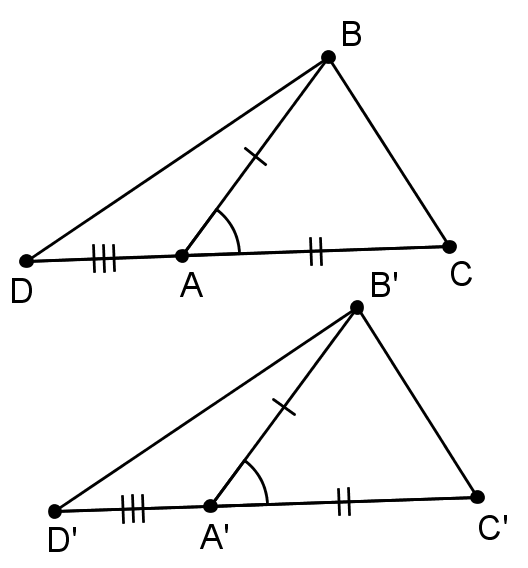
\includegraphics[width=5cm]{BILDER/1-2-13-Nebenwinkel.png}}
\end{proof}

% Folgendes mehr hervorheben?? Das ist ein Satz bei Hartshorne??
% Siehe seine Bemerkung ("Note") auf Seite 93, dass hier Euklid's
% I.13 ersetzt wird

Eine direkte Konsequenz des Theorems ist, dass Scheitelwinkel $\alpha$ und $\alpha'$ zueinander
kongruent sind. Sie sind nämlich beide Nebenwinkel eines Winkels $\beta$.

\begin{thm}\label{thm:satz.s1l}
    Mit den Bezeichnungen aus der Skizze gilt:

    %% Achtung: Hier sollte man vielleicht einen Text in die Aussage schreiben
    % (wie bei Hartshorne, S.93)

    \centerline{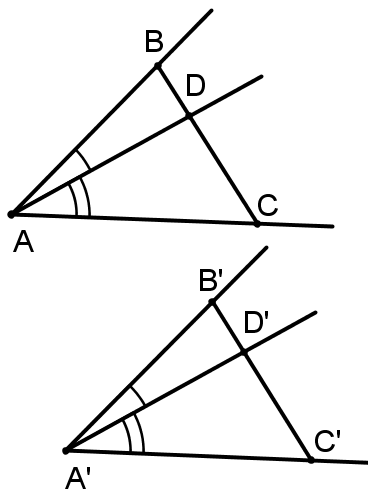
\includegraphics[width=5cm]{BILDER/1-2-15b-Winkel.png}}

    \renewcommand{\labelenumi}{\alph{enumi})} % ändert die Nummerierung von (1) auf a)
    \begin{enumerate}
        \item\label{thm:satz.s1l:item1} \emph{(Addition von Winkeln)} $\wi(BAD) \cong \wi(B'A'D')$
            und $\wi(DAC) \cong \wi(D'A'C')$\\ $\Rightarrow\;\wi(BAC) \cong \wi(B'A'C')$

        \item\label{thm:satz.s1l:item2} \emph{(Subtraktion von Winkeln)} $\wi(BAC) \cong
            \wi(B'A'C')$ und $\wi(DAC) \cong \wi(D'A'C')$\\
            $\Rightarrow\; \wi(BAD) \cong \wi(B'A'D')$
    \end{enumerate}
\end{thm}

$\wi(BAD)$ heißt die \emph{Differenz} der Winkel $\wi(BAC)$ und $\wi(DAC)$:

$$
    \wi(BAC) - \wi(DAC) := \wi(BAD).
$$

\begin{proof}
    \begin{description}
        \item[~\ref{thm:satz.s1l:item2}] Seien $B',\, C'$ so gewählt, dass $\str{AB} \cong
            \str{A'B'}$ und $\str{AC} \cong \str{A'C'} \stackrel{(SWS)}{\Longrightarrow} ABC \cong
            A'B'C'$ und daher $\wi(ABC) \cong \wi(A'B'C'),\; \wi(ACB) \cong \wi(A'C'B')$ und
            $\str{BC} \cong \str{B'C'}$ $\stackrel{(WSW)}{\Longrightarrow} ACD \cong  A'C'D'$ und
            somit $\str{CD} \cong \str{C'D'}$ und daher als Differenz kongruenter Strecken $\str{BD}
            \cong \str{B'D'}$
            % THOMAS (?) Sollte das folgende nicht \stackrel{(SWS)} sein???
            $\stackrel{(WSW)}{\Longrightarrow} BAD \cong B'A'D'$ und folglich $\wi(BAD) \cong
            \wi{B'A'D'}$.

        \item[~\ref{thm:satz.s1l:item1}] Als Nebenwinkel zu den kongruenten Winkeln $\alpha$ und
            $\alpha'$ ergibt sich wegen Theorem~\ref{thm:satz.s1k} die Kongruenz $\wi(DAE) \cong
            \wi(D'A'E')$ und daher nach ~\ref{thm:satz.s1l:item2}

            $$
                \beta = \wi(CAE) = \wi(DAE) - \wi(DAC) \cong \wi(D'A'E') - \wi(D'A'C') = \wi(C'A'E') =
                \beta'.
            $$

            Wiederum aus Theorem~\ref{thm:satz.s1k} folgt die Kongruenz $\wi(BAC) \cong \wi(B'A'C')$
            für die Nebenwinkel von $\beta$ und $\beta'$.

            \centerline{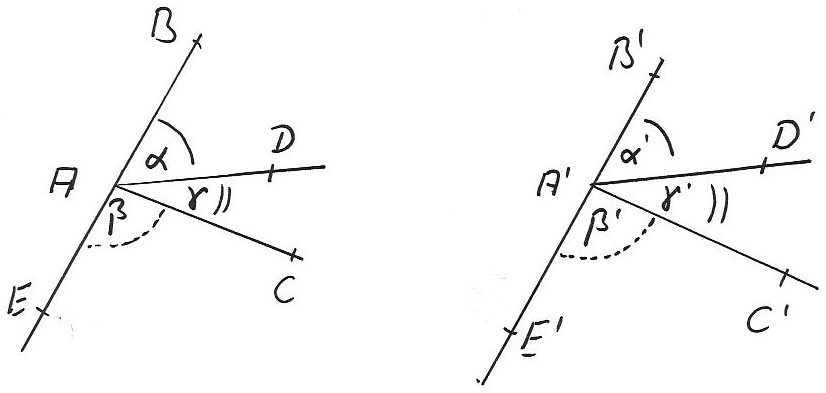
\includegraphics[width=7cm]{BILDER/1-2-15a-Winkel.jpg}}
    \end{description}
\end{proof}

\begin{defi}
    Gegeben seien zwei Winkel $\wi(BAC)$ und $\wi(EDF)$. Der Winkel $\wi(BAC)$ heißt kleiner als der
    Winkel $\wi(EDF)$, wenn es einen Strahl $\pf{DG}$ im Innern von $\wi(EDF)$ gibt, so dass
    $\wi(BAC) \cong \wi(GDF)$. $\wi(EDF)$ heißt größer als $\wi(BAC)$.
\end{defi}

\centerline{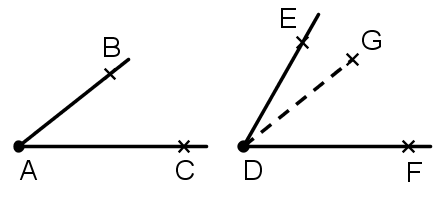
\includegraphics[width=5cm]{BILDER/1-2-16-Winkel.png}}

\begin{thm}\
    \renewcommand{\labelenumi}{\alph{enumi})} % ändert die Nummerierung von (1) auf a)
    \renewcommand{\labelenumii}{\alph{enumi}\textsubscript{\arabic{enumii}})}
        % ändert Nummerierung 2. Ebene
    \begin{enumerate}
        \item Ist $\alpha \cong \alpha'$ und $\beta \cong \beta'\;\Rightarrow$ $\{\alpha < \beta\;
            \Longleftrightarrow\; \alpha' < \beta'\}$.

        \item "`$ < $"' definiert eine Ordnung auf der Menge der Winkel, d.h.
        \begin{enumerate}
            \item $\alpha < \beta$ und $\beta < \gamma\; \Rightarrow\; \alpha < \gamma$.

            \item $\forall$ Winkel $\alpha$ und $\beta$ gilt genau eine der Beziehungen: $\alpha <
                \beta,\;\alpha \cong \beta,\;\alpha > \beta$.
        \end{enumerate}
    \end{enumerate}
\end{thm}

\begin{proof}
    Verläuft entsprechend wie der Beweis von Theorem~\ref{thm:satz.s1g} für Strecken. %(Übung?)
\end{proof}

% BEMERKUNG: Folgendes sind bei Euklid noch implizite Annahmen oder Axiome (CHECK!)

\begin{thm}\label{thm:satz.s1m}\
    \renewcommand{\labelenumi}{\alph{enumi})} % ändert die Nummerierung von (1) auf a)
    \begin{enumerate}
        \item Es gibt rechte Winkel.

        \item Je 2 rechte Winkel sind zueinander kongruent.
    \end{enumerate}
\end{thm}

\begin{proof}
    \renewcommand{\labelenumi}{\alph{enumi})} % ändert die Nummerierung von (1) auf a)
    \begin{enumerate}
        \item $C$ sei derart, dass $\str{OB} \cong \str{OC}$, $D$ sei der Schnittpunkt der Strecke
            $\str{BC}$ mit $\pf{OA}$

            \begin{enumerate}
                \item $D = O\in g(B,C)\; \Rightarrow\; \wi(BOA) \cong \wi(COA)$ und damit Rechter.

                \item $D \neq O \notin g(B,C)\; \Rightarrow\; BOD \cong COD\; \Rightarrow\; \wi(ODB)
                    \cong \wi(ODC)$ und damit Rechter.
            \end{enumerate}

            \centerline{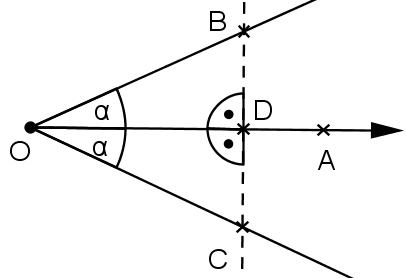
\includegraphics[width=5cm]{BILDER/1-2-18a-Winkel.png}}

        \item Angenommen, $\alpha \neq \alpha'$ seien verschiedene rechte Winkel, etwa $\alpha <
            \alpha'\; \Rightarrow$ tragen $\alpha$ am Strahl $\pf{A'B'}$ an und erhalten $\alpha
            \cong \wi(E'A'B')$ und $\pf{A'E'}$ im Innern von $\alpha'\; \Rightarrow\; C'$ im Innern
            von $\wi(E'A'D') \cong \beta\; \Rightarrow\; \beta' < \beta$.

            Jedoch: $\alpha' \cong \beta' < \beta \cong \alpha\; \Rightarrow\; \alpha' < \alpha$,
            Widerspruch.

            \centerline{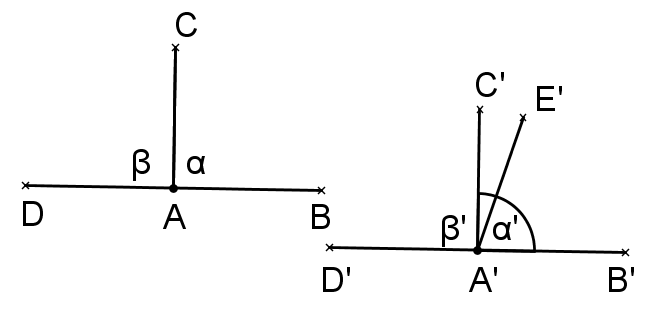
\includegraphics[width=5cm]{BILDER/1-2-18b-Winkel.png}}
    \end{enumerate}
\end{proof}

\section*{Vorlesung am 10.05.2011}

\subsection*{Beweis des SSS-Kriteriums}

Die Addition von Winkeln erlaubt auch einen Beweis des SSS-Kriteriums (Theorem~\ref{thm:satz.s1n}).
Zur Vorbereitung zunächst zwei Aussagen über gleichschenklige Dreiecke.

\begin{thm}\label{thm:lemma.l1b}
    Gilt in einem Dreieck $ABC$ die Kongruenz $\str{AC} \cong \str{BC}$, dann ist auch $\wi(CAB)
    \cong \wi(CBA)$, d.h. das Dreieck ist gleichschenklig. Umgekehrt folgt aus der Kongruenz der
    Winkel $\wi A \cong \wi B$ die Kongruenz der Seiten $\str{AC} \cong \str{BC}$.
\end{thm}
%\ref{lemma.l1b}

\begin{proof}
    Mit $B' = A,\;A' = B$ und $C' = C$ ist in beiden Fällen $ABC \cong A'B'C'$ - im 1. Fall wegen
    (SWS) und im 2. Fall wegen (WSW).
\end{proof}

\begin{thm}[Existenz gleichschenkliger Dreiecke]\label{thm:folg.f1a}
    Zu jeder Strecke $\str{AB}$ gibt es ein gleichschenkliges Dreieck mit $\str{AB}$ als Grundseite.
\end{thm}
%\ref{folg.f1a}

\begin{proof}
    Sei $\str{AB}$ gegeben und $C \notin g(A,B)$. Dann gibt es ein Dreieck $\triangle= ABC$. Wenn
    $\wi(CAB)\cong\wi(CBA)$, dann ist $\triangle$ gleichschenklig nach Theorem~\ref{thm:lemma.l1b}.
    Andernfalls sei etwa $\wi(CAB) < \wi(CBA)$.  Dann tragen wir gemäß (C4) den Winkel $\wi(CAB)$
    bei $B$ ab. Der zweite Schenkel $\pf{BE}$ schneidet nach \ref{thm:satz.s1c}. Die Strecke
    $\str{AC}$, etwa im Punkt $D$. Dann ist wieder nach Theorem~\ref{thm:lemma.l1b} $ABD$
    gleichschenklig.

    \centerline{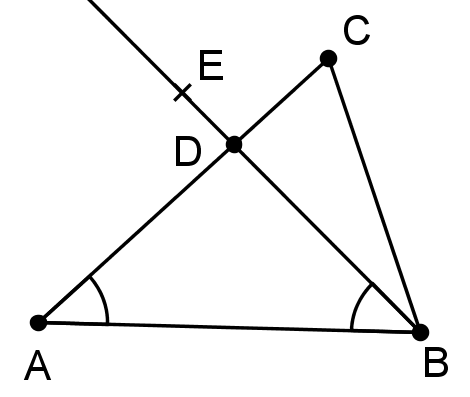
\includegraphics[width=5cm]{BILDER/1-2-20-Dreieck.png}}
\end{proof}

\begin{proof}[Beweis des SSS-Kriteriums, Theorem~\ref{thm:satz.s1n}]
    Es ist zu zeigen, dass sich die Kongruenz der Seiten auf die Winkel überträgt.

    \centerline{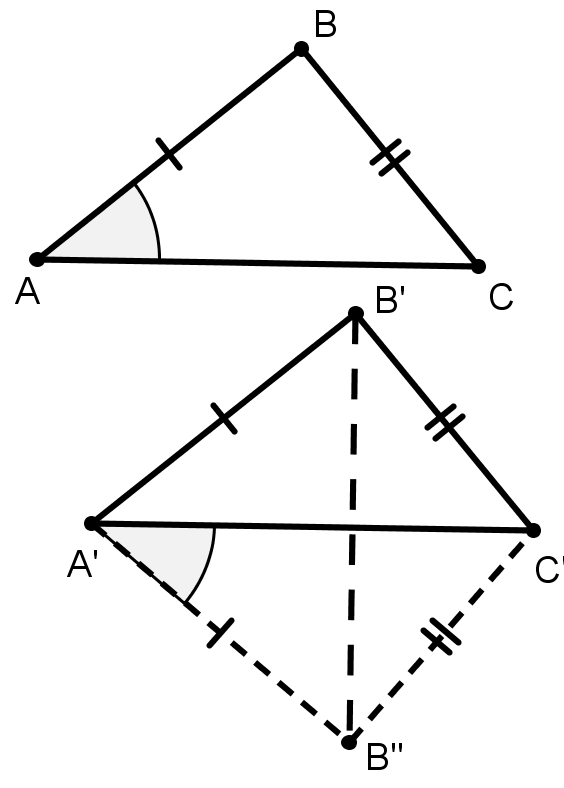
\includegraphics[width=5cm]{BILDER/1-2-21-SSS.png}}

    Sei $B''$ derart, dass $\wi(BAC) \cong \wi(B''A'C')$ und $\str{AB} \cong \str{A'B''}$

    $\stackrel{(SWS)}{\Longrightarrow}\; ABC \cong A'B''C'\; \Rightarrow\;\str{BC} \cong
    \str{B''C'}$

    $B'A'B''$ und $B'C'B''$ sind gleichschenklig\\
    $\Longrightarrow$ (Theorem~\ref{thm:lemma.l1b}) $\wi(A'B'B'') \cong \wi(A'B''B')$

    genauso: $\wi(C'B'B'') \cong \wi(C'B''B')$

    $\Longrightarrow\; (\ref{thm:satz.s1l:item1}$ (Addition der Winkel)

    $\wi(A'B'C') \cong \wi(A'B''C') \cong \wi(ABC)$

    $\stackrel{(SWS)}{\Longrightarrow}\; A'B''C' \cong A'B'C'$.

    Aus $ABC \cong A'B''C'$ folgt $ABC \cong A'B'C'$
\end{proof}

%\subsection*{Kongruenz von Strecken und Winkeln in der Poincaréschen
%Kreisscheibe?}

%\section*{Vorlesung am 12.05.2011}

%\subsection*{Literatur}
%\cite[Kapitel 1 und 2]{SS-2005},
%\cite[Chapter 1]{stillwell-2005},
%\cite[Chapter 1]{hartshorne-2000}
%\cite[Chapter 1]{coxeter-1969}


\chapter{Descartes}
\subsection*{René Descartes}

\begin{itemize}
\item René Descartes (1596--1650) führte in seinem Werk \glqq La Géométrie\grqq\ Koordinaten in die
Geometrie ein
\item dadurch begründete er die \glqq Analytische Geometrie\grqq , die eine neue Verbindung von
Algebra und Geometrie ermöglichte
\item Geometrische Objekte ließen sich von nun an durch Gleichungen und Parametrisierungen
beschreiben
%\item Die Bedeutung dieser neuen Technik kann kaum überschätzt werden
\end{itemize}

Im Folgenden werden wir uns vor allem auf den Körper der reellen Zahlen beschränken. Sämtliche
Aussagen %???
haben ihre Gültigkeit aber auch für andere Körper. Wann immer von Ungleichungen die Rede ist, sollte
dabei ein geordneter Körper angenommen werden.

\subsection*{Kurven im $\R^2$}

Im $\R^2$ lassen sich {\em Kurven} beschreiben durch

\begin{enumerate}
\item[1)] Gleichungen

\begin{itemize}
\item lineare Gleichungen $a x + b y + c = 0$ mit $(a,b) \not = 0$ beschreiben Geraden
\item Kreise werden durch spezielle quadratischen Gleichungen $(x-a)^2 + (y-b)^2 - c^2 = 0$
beschrieben

%\item Gleichungen höheren Gerades sind auch von Interesse;
% Elliptische Kurven sind spezielle Kurven vom Grad $3$ die zum
% Beispiel in der Krytologie eine wichtige Rolle spielen

\end{itemize}

\item[2)] Parametrisierungen / Parameterdarstellungen

\begin{itemize}
\item Geraden werden parametrisiert mit Hilfe von Vektoren %einen Ortsvektor und einen Richtungsvektor
$$\left\{ \ve(xyz)\right\}$$
\item Kreise lassen sich mit Hilfe trigonometrischer Funktionen
  parametrisieren
$$
\left\{  \right\}
$$
\end{itemize}

\end{enumerate}

% ACHTUNG:
% Wir fassen hier den $\R^2$ als Vektorraum von Spaltenvektoren auf...


Die {\em algebraische Geometrie} befasst sich mit Darstellungen
geometrischer Objekte ({\em algebraischen Varietäten}) die als
Nullstellengebilde von Polynomgleichungen auftreten.


Die {\em Differentialgeometrie} befasst sich mit Parametrisierungen
geometrischer Objekte ({\em Mannigfaltigkeiten}) und daraus
abgeleiteten Eigenschaften.%, wie Krümmung


\medskip

{\bf To be filled: Ungleichungen bzw. zusätzliche Parameter 
ermöglichen die Beschreibung von Punkten im Inneren eines Kreises oder
auf einer Seite einer Geraden, etc...}





\subsection*{Lineare Algebra revisted}

Die Linearen Algebra befasst sich mit linearen Gleichungssystemen und
Parameterdarstellungen Ihrer Lösungen.

{\bf to be filled!}




\subsection*{Affine Geometrie}


\begin{defi}
Seien $x_1,\dots,x_m\in\R^n$ und
$\lambda_1,\dots,\lambda_m\in\R$. Dann heißt die Linearkombination
$x=\sum_{i=1}^m\lambda_i\,x_i $ genau dann 
{\em Affinkombination}, wenn $\sum_{i=1}^m\lambda_i = 1$.
\end{defi}



\begin{defi}
$x_1,\dots,x_m\in\R^n$ heißen
{\em affin (un)anhängig}, falls es
$(\lambda_1,\dots,\lambda_m)\in\R^m\setminus\{0\}$ gibt mit
$\sum_{i=1}^m\lambda_i = 0$ und $x=\sum_{i=1}^m\lambda_i\,x_i = 0$.
\end{defi}


\begin{thm}
$x_1,\dots,x_m\in\R^n$ sind genau dann affin unabhängig,
\begin{itemize}
\item
wenn sich keines der $x_i$ als Affinkombination der anderen $x_j$,
$j\not= i$, schreiben lässt.

\item
wenn $\begin{pmatrix}x_1\\1\end{pmatrix},\dots,\begin{pmatrix}x_m\\1\end{pmatrix}\in\R^{n+1}$ linear unabhängig sind
\end{itemize}
\end{thm}


%% ACHTUNG: Hier könnte man auch gut eine "affine Basis" einführen,
%% als maximal affin unabhängige Menge...




\section*{Vorlesung am 31.05.2011}







%%% Local Variables: 
%%% mode: latex
%%% TeX-master: "AxiomatischeGeometrie"
%%% End: 


\chapter{Desargues}
%Zitat von Arthur Cayley (1821-1895): "All geometry is projective geometry"
% siehe Wallner, Pottmann, Seite 1

\subsection*{Gérard Desargues}

%%% Local Variables: 
%%% mode: latex
%%% TeX-master: "AxiomatischeGeometrie"
%%% End: 


% BIBLIOGRAPHY
%  --> Erzeugung durch Aufruf von ``bibtex AxiomatischeGeometrie''

\cleardoublepage % Beendet eine Seite und erzwingt auf den nachfolgenden Seiten die Ausgabe aller
    % Gleitobjekte (z.B. Abbildungen), die bislang definiert, aber noch nicht ausgegeben wurden.
    % Dieser Befehl fügt, falls nötig, eine leere Seite ein, sodaß die nächste Seite nach den
    % Gleitobjekten eine ungerade Seitennummer hat.

\phantomsection
\nocite{*}
\bibliographystyle{plain}
\bibliography{AxiomatischeGeometrieBiblio.bib}

\end{document}

% INDEX ???

%\newpage % to get page for index right in table of contents?

%\cleardoublepage
%\phantomsection
%\printindex

\end{document}
